\part{Set Theory, Logic, and Foundations}

Foundational prerequisites collect the logical, set-theoretic, functional, order-theoretic, cardinal, and research-practice language used throughout the notes.

\section{Sets}

Sets provide the membership language used throughout the notes: elements, subsets, products, power sets, operations, and indexed families.

\subsection{Introduction to Sets}

\begin{definition} \label{def:sets-and-membership} \hlt{Sets and Membership}\\
Sets are treated as primitive objects. For an object $x$ and a set $E$, write $x\in E$ when $x$ is an \hlt{element} of $E$, and write $x\notin E$ otherwise. The \hlt{empty set} $\emptyset$ has no elements.
\end{definition}

\begin{definition} \hlt{Set-Builder Notation}\\
For a set $X$ and a condition $P(x)$ on its elements, $\{x\in X:P(x)\}$ denotes the set of $x\in X$ satisfying $P(x)$.
\end{definition}


\subsection{Cartesian Products}

\begin{definition} \label{def:cartesian-product} \hlt{Cartesian Product}\\
For sets $X$ and $Y$, the \hlt{Cartesian product} is $X\times Y\defeq\{(x,y):x\in X,\ y\in Y\}$.\\
The order matters: the first coordinate comes from $X$, and the second comes from $Y$.
\end{definition}

\begin{definition} \label{def:indexed-cartesian-product} \hlt{Cartesian Product of an Indexed Family}\\
Let $\{E_i\}_{i\in I}$ be an indexed family of sets and set $U\defeq\bigcup\limits_{i\in I}E_i$.\\
The \hlt{Cartesian product} is $\prod\limits_{i\in I}E_i\defeq\{x:I\to U:\forall i\in I,\ x(i)\in E_i\}$.
\begin{enumerate}[label=(\roman*)]
\setlength{\itemsep}{0pt}
\item If $I=\{1,2\}$, then $x\mapsto(x(1),x(2))$ gives the canonical bijection $\prod\limits_{i\in\{1,2\}}E_i\cong E_1\times E_2$.
\item If $E_i=E$ for every $i\in I$, then $\prod\limits_{i\in I}E_i=E^I=\{x:I\to E\}$.
\end{enumerate}
\end{definition}

\begin{figure}[H]
    \centering
    \begin{tikzpicture}[
  >=Stealth,
  every node/.style={font=\small},
  axis/.style={->, gray!65, line width=0.45pt},
  interval/.style={line width=1.2pt},
  product/.style={draw=blue!60!black, fill=blue!8, line width=0.55pt},
  guide/.style={gray!55, dashed, line width=0.4pt},
  point/.style={circle, fill=black, inner sep=1.2pt}
]
  \draw[axis] (-0.25,0) -- (5.3,0);
  \draw[axis] (0,-0.25) -- (0,3.5);

  \coordinate (A0) at (1.15,0);
  \coordinate (A1) at (4.55,0);
  \coordinate (B0) at (0,0.8);
  \coordinate (B1) at (0,2.85);

  \draw[product] (1.15,0.8) rectangle (4.55,2.85);
  \draw[interval, blue!60!black] (A0) -- (A1);
  \draw[interval, orange!75!black] (B0) -- (B1);

  \node[below=5pt, blue!60!black] at (4.25,0) {$A$};
  \node[left=5pt, orange!75!black] at (0,2.75) {$B$};
  \node[blue!55!black, anchor=south east] at (4.35,0.92) {$A\times B$};

  \coordinate (P) at (2.75,2.05);
  \draw[guide] (2.75,0) -- (P);
  \draw[guide] (0,2.05) -- (P);
  \node[point] at (P) {};
  \node[below=1pt] at (2.75,0) {$a$};
  \node[left=2pt] at (0,2.05) {$b$};
  \node[above right=2pt] at (P) {$(a,b)$};
\end{tikzpicture}

    \caption{$A\times B$: first coordinate in $A$, second in $B$.}
    \label{fig:cartesian-product-rectangle}
\end{figure}


\subsection{Subsets and Power Sets}

\begin{definition} \label{def:proper-subsets-singletons-and-nonempty} \hlt{Basic Subset Terminology}\\
Let $A,B$ be sets. Write $A\subseteq B$; $A=B$ iff $A\subseteq B$ and $B\subseteq A$.
\begin{enumerate}[label=(\roman*)]
\setlength{\itemsep}{0pt}
\item $A$ is a \hlt{proper subset} of $B$, written $A\subsetneq B$, iff $A\subseteq B$ and $A\neq B$.
\item $A$ is a \hlt{singleton} iff $\exists x$ such that $A=\{x\}$.
\item $A$ is \hlt{nonempty} iff $A\neq\emptyset$.
\end{enumerate}
\end{definition}

\begin{method} \label{meth:proof-by-containment} \hlt{Proof by Two Containments}\\
To prove $A=B$, prove both inclusions.
\begin{enumerate}[label=(\roman*)]
\setlength{\itemsep}{0pt}
\item To prove $A\subseteq B$, let $x\in A$ be arbitrary and use the definitions and hypotheses to show $x\in B$.
\item To prove $B\subseteq A$, let $x\in B$ be arbitrary and use the definitions and hypotheses to show $x\in A$.
\item Once both containments are proved, conclude $A=B$ by extensionality of sets.
\end{enumerate}
If both sides are described by membership conditions, this is a chain, $x\in A \Longleftrightarrow \cdots \Longleftrightarrow x\in B$.
\end{method}

\begin{definition} \label{def:power-set} \hlt{Power Set}\\
For a set $X$, the \hlt{power set} is $\mathcal{P}(X)\defeq\{S:S\subseteq X\}$.
\end{definition}

\begin{example} \label{ex:small-power-sets} \hlt{Small Power Sets}
\begin{enumerate}[label=(\roman*)]
\setlength{\itemsep}{0pt}
\item If $X=\emptyset$, then $\mathcal{P}(X)=\{\emptyset\}$.
\item If $X=\{a,b\}$ with $a\neq b$, then $\mathcal{P}(X)=\{\emptyset,\{a\},\{b\},X\}$.
\end{enumerate}
Hence $S\in\mathcal{P}(X)$ iff $S\subseteq X$; membership in $\mathcal{P}(X)$ is containment in $X$.
\end{example}


\subsection{Union, Intersection, Difference, and Complement}

\begin{definition} \label{def:analysis-sets-and-operations} \hlt{Elementary Set Operations}\\
Let $X$ be a set and let $A,B\subseteq X$.
\begin{enumerate}[label=(\roman*)]
\setlength{\itemsep}{0pt}
\item \hlt{Union}: $A\cup B\defeq\{x\in X:x\in A\text{ or }x\in B\}$.
\item \hlt{Intersection}: $A\cap B\defeq\{x\in X:x\in A\text{ and }x\in B\}$.
\item \hlt{Difference}: $A\setminus B\defeq\{x\in X:x\in A\text{ and }x\notin B\}$.
\item \hlt{Complement}: $A^c\defeq X\setminus A$, relative to the ambient set $X$.
\end{enumerate}
\end{definition}

\begin{definition} \label{def:symmetric-difference-of-events-and-sets} \hlt{Symmetric Difference}\\
Let $X$ be a set and let $A,B\subseteq X$.
The \hlt{symmetric difference} is $A\triangle B\defeq(A\setminus B)\cup(B\setminus A)$.\\
It consists exactly of the elements belonging to one of $A$ and $B$, but not both.
\end{definition}

\begin{proposition} \label{prop:analysis-set-algebra} \hlt{Basic Set Algebra}\\
Let $X$ be a set and let $A,B,C\subseteq X$. Then
\begin{enumerate}[label=(\roman*)]
\setlength{\itemsep}{0pt}
\item $A\cap(B\cup C)=(A\cap B)\cup(A\cap C)$;
\item $A\cup(B\cap C)=(A\cup B)\cap(A\cup C)$;
\item $(A\cup B)^c=A^c\cap B^c$;
\item $(A\cap B)^c=A^c\cup B^c$;
\item $A\triangle B=(A\cup B)\setminus(A\cap B)$.
\end{enumerate}
\begin{proof}
Fix an arbitrary $x\in X$.
By set extensionality, each identity follows once its two membership conditions are equivalent.
\begin{enumerate}[label=(\roman*)]
\setlength{\itemsep}{0pt}
\item[(i)] Membership in $A\cap(B\cup C)$ means that $x\in A$ and that either $x\in B$ or $x\in C$.
This holds exactly when either $x\in A\cap B$ or $x\in A\cap C$.
Hence it is equivalent to membership in $(A\cap B)\cup(A\cap C)$.
\item[(ii)] Membership in $A\cup(B\cap C)$ means that $x\in A$, or that both $x\in B$ and $x\in C$.
This holds exactly when two conditions are satisfied.
First, $x\in A$ or $x\in B$; second, $x\in A$ or $x\in C$.
Hence it is equivalent to membership in $(A\cup B)\cap(A\cup C)$.
\item[(iii)] The condition $x\in(A\cup B)^c$ is equivalent to $x\notin A\cup B$.
This means that $x\notin A$ and $x\notin B$, or equivalently $x\in A^c\cap B^c$.
\item[(iv)] The condition $x\in(A\cap B)^c$ is equivalent to $x\notin A\cap B$.
This means that $x\notin A$ or $x\notin B$, or equivalently $x\in A^c\cup B^c$.
\item[(v)] The condition $x\in A\triangle B$ is equivalent to $x\in A\setminus B$ or $x\in B\setminus A$.
Thus $x$ belongs to one of $A$ and $B$, but not both.
Equivalently, $x\in A\cup B$ and $x\notin A\cap B$.
By the definition of difference, this is equivalent to $x\in(A\cup B)\setminus(A\cap B)$.
\end{enumerate}
\hlt{Structural Commentary}: Each identity reduces to an equivalence of membership conditions.\\
\hlt{Key Insight}: Membership turns set operations into logical connectives.\\
\end{proof}
\end{proposition}

\begin{illustrationfigure}[H]
    \centering
    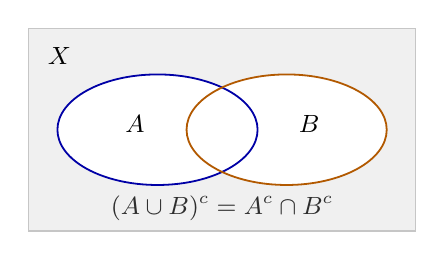
\begin{tikzpicture}[
  x=0.82cm,
  y=0.78cm,
  every node/.style={font=\small},
  ambient/.style={draw=gray!45, fill=gray!12, line width=0.5pt},
  setA/.style={draw=blue!65!black, line width=0.65pt},
  setB/.style={draw=orange!70!black, line width=0.65pt}
]
  \draw[ambient] (-3,-1.65) rectangle (3,1.65);
  \fill[white] (-1.0,0) ellipse (1.55 and 0.9);
  \fill[white] (1.0,0) ellipse (1.55 and 0.9);
  \draw[setA] (-1.0,0) ellipse (1.55 and 0.9);
  \draw[setB] (1.0,0) ellipse (1.55 and 0.9);

  \node at (-1.35,0.1) {$A$};
  \node at (1.35,0.1) {$B$};
  \node[anchor=north west] at (-2.85,1.5) {$X$};
  \node[gray!35!black] at (0,-1.28) {$(A\cup B)^c=A^c\cap B^c$};
\end{tikzpicture}

    \caption{The shaded region represents $(A\cup B)^c=A^c\cap B^c$ inside the ambient set $X$.}
    \label{fig:de-morgan-complement-union}
\end{illustrationfigure}

Figure \ref{fig:de-morgan-complement-union} illustrates part (iii).
The shaded region lies outside both $A$ and $B$, so it is outside $A\cup B$.


\subsection{Indexed Families and Products}

\begin{definition} \label{def:indexed-families-unions-intersections} \hlt{Families, Indexed Families, Unions, and Intersections}\\
Let $X$ be a set and let $I$ be an index set.
\begin{enumerate}[label=(\roman*)]
\setlength{\itemsep}{0pt}
\item A \hlt{family} or \hlt{collection} of sets is a set whose members are sets.
\item An \hlt{indexed family} in $X$ over $I$ is a map $A:I\to\mathcal{P}(X)$; write $A_i\defeq A(i)$ and $\{A_i\}_{i\in I}$.
\item For an indexed family $\{A_i\}_{i\in I}$ in $X$, $\bigcup\limits_{i\in I}A_i\defeq\{x\in X:\exists i\in I,\ x\in A_i\}$.
\item For an indexed family $\{A_i\}_{i\in I}$ in $X$, $\bigcap\limits_{i\in I}A_i\defeq\{x\in X:\forall i\in I,\ x\in A_i\}$.
\end{enumerate}
Union corresponds to $\exists i\in I$; intersection corresponds to $\forall i\in I$.
\end{definition}

\begin{theorem} \label{thm:metric-de-morgan-laws} \hlt{Arbitrary De Morgan Laws}\\
Let $X$ be a set. For any collection $\{E_\alpha\}$ of subsets of $X$, $\left(\bigcup\limits_\alpha E_\alpha\right)^c=\bigcap\limits_\alpha E_\alpha^c$ and $\left(\bigcap\limits_\alpha E_\alpha\right)^c=\bigcup\limits_\alpha E_\alpha^c$.
\begin{proof}
The first identity follows from membership: $x\in\left(\bigcup\limits_\alpha E_\alpha\right)^c$ $\Longleftrightarrow$ $x\notin E_\alpha \ \forall \alpha$ $\Longleftrightarrow$ $x\in\bigcap\limits_\alpha E_\alpha^c$.\\
The second follows by applying the first identity to the complements $E_\alpha^c$, or by the same membership argument.\\
\hlt{Structural Commentary}: Complements exchange unions and intersections.\\
\hlt{Key Insight}: Negating ``for some'' gives ``for every'', and conversely.
\end{proof}
\end{theorem}

\begin{definition} \label{def:disjoint-families-and-parametrizations} \hlt{Disjoint Families and Parametrizations}\\
Let $\mathcal{F}$ be a family of sets and let $\{A_i\}_{i\in I}$ be an indexed family.
\begin{enumerate}[label=(\roman*)]
\setlength{\itemsep}{0pt}
\item A family $\mathcal{F}$ is \hlt{pairwise disjoint} iff $E,F\in\mathcal{F}$ and $E\neq F$ imply $E\cap F=\emptyset$.
\item An indexed family $\{A_i\}_{i\in I}$ \hlt{parametrizes} a family $\mathcal{F}$ iff $\mathcal{F}=\{A_i:i\in I\}$.
\end{enumerate}
\end{definition}

\begin{definition} \label{def:indexed-cartesian-product} \hlt{Cartesian Product of an Indexed Family}\\
Let $\{E_i\}_{i\in I}$ be an indexed family of sets and set $U\defeq\bigcup\limits_{i\in I}E_i$.\\
The \hlt{Cartesian product} is $\prod\limits_{i\in I}E_i\defeq\{x:I\to U:\forall i\in I,\ x(i)\in E_i\}$.
\begin{enumerate}[label=(\roman*)]
\setlength{\itemsep}{0pt}
\item If $I=\{1,2\}$, then $x\mapsto(x(1),x(2))$ gives the canonical bijection $\prod\limits_{i\in\{1,2\}}E_i\cong E_1\times E_2$.
\item If $E_i=E$ for every $i\in I$, then $\prod\limits_{i\in I}E_i=E^I=\{x:I\to E\}$.
\end{enumerate}
Different parametrizations of the same family may give different indexed products.
\end{definition}


\subsection{Russell's Paradox and Axioms}

\begin{theorem} \label{thm:russells-paradox} \hlt{Russell's Paradox}\\
For a condition $P(x)$ on sets, unrestricted comprehension asserts $(\exists R)(\forall x)\,[x\in R\Longleftrightarrow P(x)]$.
\begin{enumerate}[label=(\roman*)]
\setlength{\itemsep}{0pt}
\item No set $R$ satisfies $(\forall x)\,[x\in R\Longleftrightarrow x\notin x]$.
\item The unrestricted comprehension schema is inconsistent.
\end{enumerate}
\begin{proof}
\begin{enumerate}[label=(\roman*)]
\setlength{\itemsep}{0pt}
\item Suppose that such a set $R$ exists. Setting $x=R$ gives $R\in R\Longleftrightarrow R\notin R$. If $R\in R$, then $R\notin R$; if $R\notin R$, then $R\in R$.\\
Both cases are contradictory, so no such set exists.
\item Take $P(x)\defeq x\notin x$.
The corresponding instance asserts
$(\exists R)(\forall x)\,[x\in R\Longleftrightarrow x\notin x]$.
This contradicts (i), proving (ii).
\end{enumerate}
\hlt{Structural Commentary}: Specialize at $x=R$, then apply the matching comprehension instance.\\
\hlt{Key Insight}: Self-membership makes the defining condition assert its own negation.\\
\end{proof}
\end{theorem}

\begin{perspective} \label{per:zfc-axiom-role-map} \hlt{From Comprehension to Axioms}\\
The obstruction in Theorem \ref{thm:russells-paradox} explains the need for controlled set formation.\\
Separation forms $\{x\in B:P(x)\}$ only after a bounding set $B$ is available.
The standard ZFC axioms have the following informal roles.
\begin{enumerate}[label=(\roman*)]
\setlength{\itemsep}{0pt}
\item \hlt{Extensionality} makes membership determine set equality.
\item \hlt{Separation} extracts a condition-defined subset from an existing bounding set.
\item \hlt{Pairing} supplies $\{a,b\}$ from given sets $a$ and $b$, including $\{a\}$ when $a=b$.
\item \hlt{Union} collects into one set the elements of the members of a given set.
\item \hlt{Power set} supplies $\mathcal{P}(A)$, the set of all subsets of a given set $A$.
\item \hlt{Infinity} supplies an inductive set from which the natural numbers are constructed.
\item \hlt{Replacement} forms the image of a set under a definable functional relation.
\item \hlt{Foundation} requires nonempty sets to contain an $\in$-minimal member.
\item \hlt{Choice} supplies a choice function on a set-indexed family of nonempty sets.
\end{enumerate}
This perspective is a functional map, not a formal axiom list or a source of proof authority.\\
Formal statements and dependencies belong to the advanced set-theory section.
\end{perspective}


\section{Logic and Proofs}

Logic fixes the grammar of mathematical statements before the notes use that grammar for definitions, theorems, and proofs.

\subsection{Statements and Well-Formed Language}

\begin{principle} \label{princ:well-formed-statements-and-bound-variables} \hlt{Well-Formed Statements}\\
A mathematical statement is well formed only after every symbol has a declared role and every expression has a defined meaning.
\end{principle}


\subsection{Connectives, Conditionals, and Truth Tables}

\hlt{Placeholder}: Add the truth-functional meanings of $\land,\lor,\neg,\Rightarrow,\Longleftrightarrow$, inclusive ``or'', truth tables, logical equivalence, converse, inverse, and contrapositive.


\subsection{Quantifiers, Bound Variables, and Negation}

\begin{principle} \label{princ:analysis-language-as-structure} \hlt{Language Carries Structure}\\
Objects, hypotheses, conclusions, and quantifier order matter. For instance,
\begin{align}
\forall x\in X\ \exists y\in Y\ P(x,y), \qquad
\exists y\in Y\ \forall x\in X\ P(x,y) \nonumber
\end{align}
are different: in the first $y$ may depend on $x$; in the second one $y$ works for all $x$.
\end{principle}

\begin{method} \label{meth:proof-grammar-and-negation} \hlt{Proof Grammar and Negation}\\
In theorem statements, put the hypotheses before the conclusion and keep quantifiers in the order meant.\\
In particular, switching $\forall$ and $\exists$ usually changes the statement; see Principle \ref{princ:analysis-language-as-structure}.\\
Before applying a rule, also check that the displayed expressions are well formed; an undefined expression makes the sentence ill formed, not merely false.\\
The word ``or'' is inclusive in mathematics, and the basic negation rules are
\begin{align}
\neg(a\land b)\Longleftrightarrow \neg a\lor\neg b, \qquad \neg(a\lor b)\Longleftrightarrow \neg a\land\neg b, \qquad \neg(a\Rightarrow b)&\Longleftrightarrow a\land\neg b \nonumber
\end{align}
Thus a proof by contradiction of $a\Rightarrow b$ assumes both $a$ and $\neg b$ and derives an impossibility.\\
\hlt{Key Insight}: Before proving or negating a statement, parse its quantifiers and logical connectives.
\end{method}

\hlt{Placeholder}: Add negation rules for quantified statements and examples translating English into symbolic logic.


\subsection{Proof Grammar and Inference}

\hlt{Placeholder}: Add inference rules such as modus ponens, universal instantiation, existential introduction, and proof templates for definitions.


\subsection{Proof by Contradiction}

\begin{method} \label{meth:proof-by-contradiction} \hlt{Proof by Contradiction}\\
By Principle \ref{princ:connectives-and-negation}, a proof by contradiction of $a\Rightarrow b$ assumes both $a$ and $\neg b$ and derives an impossibility.
\end{method}


\subsection{Mathematical Induction and Well-Ordering}

\begin{principle} \label{princ:mathematical-induction} \hlt{Mathematical Induction}\\
Let $P_1,P_2,\ldots$ be statements indexed by positive integers. To prove $P_n$ for every $n\in\N$, it is enough to prove:
\begin{enumerate}[label=(\roman*)]
\setlength{\itemsep}{0pt}
\item \hlt{basis}: $P_1$ is true;
\item \hlt{induction step}: for every $n\in\N$, $P_n$ implies $P_{n+1}$.
\end{enumerate}
The induction step is an implication; it does not prove $P_{n+1}$ in isolation.\\
The basis starts the chain, and the implication carries truth from one statement to the next.
\end{principle}

\begin{principle} \label{princ:well-ordering-natural-numbers} \hlt{Well-Ordering of $\N$}\\
Every nonempty subset of $\N$ has a least element, justifying first unused indices, first repeated values, and increasing listings of infinite subsets of $\N$.
\end{principle}


\section{Functions}

Functions assign unique outputs; their images, preimages, restrictions, compositions, and inverses organize nearly every later construction.

\subsection{Functions, Images, and Preimages}

\begin{definition} \label{def:functions-images-preimages} \hlt{Functions, Images, and Preimages}\\
Let $X,Y$ be sets. A \hlt{function} $f:X\to Y$ assigns a unique value $f(x)\in Y$ to each $x\in X$.
\begin{enumerate}[label=(\roman*)]
\setlength{\itemsep}{0pt}
\item $X=\operatorname{dom}(f)$ is the \hlt{domain}, and $Y$ is the \hlt{codomain}.
\item $\operatorname{range}(f)\defeq f(X)\defeq\{f(x):x\in X\}$ is the \hlt{range} of $f$.
\item If $A\subseteq X$, then $f(A)\defeq\{f(x):x\in A\}$ is the \hlt{image} of $A$.
\item If $B\subseteq Y$, then $f^{-1}(B)\defeq\{x\in X:f(x)\in B\}$ is the \hlt{preimage} of $B$; no inverse function is required.
\end{enumerate}
\end{definition}

\begin{assumption} \label{assump:function-extensionality} \hlt{Function Extensionality}\\
Let $X,Y$ be sets and let $f,g:X\to Y$. If $(\forall x\in X)\,f(x)=g(x)$, then $f=g$.
\end{assumption}

\begin{proposition} \label{prop:image-preimage-calculus} \hlt{Image and Preimage Calculus}\\
Let $X,Y,I$ be sets with $I\neq\emptyset$, and let $f:X\to Y$. Let $\{A_i\}_{i\in I}$ and $\{B_i\}_{i\in I}$ be indexed families in $X$ and $Y$, respectively.
\begin{enumerate}[label=(\roman*)]
\setlength{\itemsep}{0pt}
\item $f\left(\bigcup\limits_{i\in I}A_i\right)=\bigcup\limits_{i\in I}f(A_i)$.
\item $f\left(\bigcap\limits_{i\in I}A_i\right)\subseteq\bigcap\limits_{i\in I}f(A_i)$.
\item $f^{-1}\left(\bigcup\limits_{i\in I}B_i\right)=\bigcup\limits_{i\in I}f^{-1}(B_i)$.
\item $f^{-1}\left(\bigcap\limits_{i\in I}B_i\right)=\bigcap\limits_{i\in I}f^{-1}(B_i)$.
\item $(\forall B\subseteq Y)\,f^{-1}(Y\setminus B)=X\setminus f^{-1}(B)$.
\item $(\forall B,C\subseteq Y)\,f^{-1}(B\setminus C)=f^{-1}(B)\setminus f^{-1}(C)$.
\item $(\forall B\subseteq Y)\,f(f^{-1}(B))=B\cap\operatorname{range}(f)$.
\item $(\forall A\subseteq X)(\forall B\subseteq Y)\,[f(A)\subseteq B\Longleftrightarrow A\subseteq f^{-1}(B)]$.
\end{enumerate}
\begin{proof}
\begin{enumerate}[label=(\roman*)]
\setlength{\itemsep}{0pt}
\item Fix $y\in Y$. Then $y\in f\left(\bigcup\limits_{i\in I}A_i\right)\Longleftrightarrow(\exists i\in I)(\exists x\in A_i)\,y=f(x)$. This is equivalent to $y\in\bigcup\limits_{i\in I}f(A_i)$.
\item If $y\in f\left(\bigcap\limits_{i\in I}A_i\right)$, choose $x\in\bigcap\limits_{i\in I}A_i$ with $y=f(x)$. Then $(\forall i\in I)\,x\in A_i$, so $(\forall i\in I)\,y\in f(A_i)$ and $y\in\bigcap\limits_{i\in I}f(A_i)$.
\item Fix $x\in X$. Then $x\in f^{-1}\left(\bigcup\limits_{i\in I}B_i\right)\Longleftrightarrow(\exists i\in I)\,f(x)\in B_i$. This is equivalent to $(\exists i\in I)\,x\in f^{-1}(B_i)$, hence to $x\in\bigcup\limits_{i\in I}f^{-1}(B_i)$.
\item Fix $x\in X$. Then $x\in f^{-1}\left(\bigcap\limits_{i\in I}B_i\right)\Longleftrightarrow(\forall i\in I)\,f(x)\in B_i$. This is equivalent to $(\forall i\in I)\,x\in f^{-1}(B_i)$, hence to $x\in\bigcap\limits_{i\in I}f^{-1}(B_i)$.
\item Fix $B\subseteq Y$ and $x\in X$. Then $x\in f^{-1}(Y\setminus B)\Longleftrightarrow f(x)\notin B\Longleftrightarrow x\notin f^{-1}(B)\Longleftrightarrow x\in X\setminus f^{-1}(B)$.
\item Fix $B,C\subseteq Y$ and $x\in X$. Then $x\in f^{-1}(B\setminus C)\Longleftrightarrow[f(x)\in B\land f(x)\notin C]$. This is equivalent to $x\in f^{-1}(B)\setminus f^{-1}(C)$.
\item Fix $B\subseteq Y$ and $y\in Y$. Then $y\in f(f^{-1}(B))\Longleftrightarrow(\exists x\in X)\,[f(x)\in B\land y=f(x)]$. This is equivalent to $y\in B\cap\operatorname{range}(f)$.
\item[$(viii)$]$(\Rightarrow)$ Fix $A\subseteq X$ and $B\subseteq Y$. Suppose $f(A)\subseteq B$ and fix $x\in A$. Then $f(x)\in B$, so $x\in f^{-1}(B)$; hence $A\subseteq f^{-1}(B)$. 
\item[$(viii)$]$(\Leftarrow)$ Fix $A\subseteq X$ and $B\subseteq Y$. Suppose $A\subseteq f^{-1}(B)$ and fix $y\in f(A)$. Choose $x\in A$ with $y=f(x)$.\\
Then $x\in f^{-1}(B)$, so $y=f(x)\in B$ and $f(A)\subseteq B$.
\end{enumerate}
\hlt{Structural Commentary}: Membership chains prove the identities; direct containments prove the adjunction.\\
\hlt{Key Insight}: Preimages translate codomain membership into domain membership.
\end{proof}
\end{proposition}

\begin{illustrationfigure}[H]
  \centering
  \begin{tikzpicture}[
  x=0.78cm,
  y=0.78cm,
  >=Stealth,
  every node/.style={font=\small},
  ambient/.style={draw=gray!35, line width=0.45pt},
  setregion/.style={draw=blue!65!black, fill=blue!8, line width=0.55pt},
  preimage/.style={draw=orange!75!black, fill=orange!12, line width=0.55pt},
  targetset/.style={draw=orange!75!black, fill=orange!10, line width=0.55pt},
  image/.style={draw=blue!65!black, fill=blue!14, line width=0.55pt},
  maparrow/.style={->, gray!58, line width=0.42pt},
  point/.style={circle, fill=gray!75, inner sep=1.25pt}
]
  \draw[ambient, fill=white] (0,0) rectangle (4.25,3.4);
  \draw[ambient, fill=gray!12] (5.65,0) rectangle (9.9,3.4);

  \node[anchor=north west] at (0.25,3.25) {$X$};
  \node[anchor=north west] at (5.9,3.25) {$Y$};

  \draw[preimage]
    plot[smooth cycle, tension=0.7] coordinates {
      (0.86,0.78)
      (0.76,1.52)
      (1.16,2.32)
      (2.03,2.72)
      (3.04,2.42)
      (3.48,1.55)
      (3.05,0.75)
      (1.86,0.48)
    };
  \node[orange!55!black] at (2.08,2.43) {$f^{-1}(B)$};

  \draw[setregion]
    plot[smooth cycle, tension=0.75] coordinates {
      (1.28,1.02)
      (1.27,1.58)
      (1.62,2.02)
      (2.25,2.08)
      (2.78,1.74)
      (2.72,1.10)
      (2.05,0.82)
    };
  \node[blue!60!black] at (2.02,1.47) {$A$};

  \draw[targetset]
    plot[smooth cycle, tension=0.75] coordinates {
      (6.38,0.72)
      (6.16,1.50)
      (6.55,2.45)
      (7.55,2.88)
      (8.72,2.55)
      (9.18,1.62)
      (8.75,0.72)
      (7.48,0.42)
    };
  \node[orange!55!black] at (8.55,2.28) {$B$};

  \draw[image]
    plot[smooth cycle, tension=0.75] coordinates {
      (6.84,1.08)
      (6.95,1.72)
      (7.45,2.06)
      (8.05,1.92)
      (8.28,1.32)
      (7.82,0.92)
      (7.20,0.88)
    };
  \node[blue!60!black] at (7.55,1.48) {$f(A)$};

  \node[point] (x1) at (1.70,1.30) {};
  \node[point] (x2) at (2.34,1.83) {};
  \node[point] (x3) at (3.04,1.95) {};
  \node[point] (x4) at (0.72,0.34) {};

  \node[point] (y1) at (7.23,1.12) {};
  \node[point] (y2) at (7.94,1.76) {};
  \node[point] (y3) at (8.56,1.98) {};
  \node[point] (y4) at (9.28,0.36) {};

  \draw[maparrow] (x1) .. controls (3.25,1.08) and (5.70,1.02) .. (y1);
  \draw[maparrow] (x2) .. controls (3.75,1.68) and (5.88,1.64) .. (y2);
  \draw[maparrow] (x3) .. controls (4.12,2.42) and (6.60,2.46) .. (y3);
  \draw[maparrow] (x4) .. controls (3.15,0.18) and (6.75,0.12) .. (y4);

  \node[gray!65] at (5.02,2.05) {$f$};
  \draw[->, gray!55, line width=0.55pt] (4.38,1.45) -- (5.48,1.45);
\end{tikzpicture}

  \caption{Image--preimage adjunction: $f(A)\subseteq B\Longleftrightarrow A\subseteq f^{-1}(B)$.}
  \label{fig:function-image-preimage}
\end{illustrationfigure}

Figure \ref{fig:function-image-preimage} illustrates Proposition \ref{prop:image-preimage-calculus}(viii). The labeled regions show that $f(A)\subseteq B$ exactly when $A\subseteq f^{-1}(B)$.

\begin{definition} \label{def:algebraic-support-of-function} \hlt{Algebraic Support of a Function}\\
Let $f:X\to Y$ and let $0\in Y$ be distinguished. The \hlt{algebraic support} of $f$ is $\operatorname{supp}(f)\defeq\{x\in X:f(x)\neq0\}$.
\end{definition}


\subsection{Injective, Surjective, and Bijective Maps}

\begin{definition} \label{def:injective-surjective-bijective} \hlt{Injective, Surjective, and Bijective Maps}\\
Let $X,Y$ be sets and let $f:X\to Y$.
\begin{enumerate}[label=(\roman*)]
\setlength{\itemsep}{0pt}
\item \hlt{Injective}: $(\forall x_1,x_2\in X)\,[f(x_1)=f(x_2)\Longrightarrow x_1=x_2]$.
\item \hlt{Surjective}: $\operatorname{range}(f)=Y$.
\item \hlt{Bijective}: $f$ is both injective and surjective.
\end{enumerate}
\end{definition}

\begin{illustrationfigure}[H]
  \centering
  \begin{tikzpicture}[
  scale=0.80,
  >=Stealth,
  every node/.style={font=\scriptsize},
  set/.style={draw=gray!65, fill=gray!10, line width=0.45pt},
  point/.style={circle, fill=black, inner sep=1.05pt},
  missed/.style={circle, fill=white, draw=black, line width=0.45pt, inner sep=1.05pt},
  map/.style={->, gray!70, line width=0.48pt}
]
  \foreach \xshift in {0,4.2,8.4} {
    \begin{scope}[xshift=\xshift cm]
      \draw[set] (0,0) ellipse (0.6 and 1.15);
      \draw[set] (2.9,0) ellipse (0.6 and 1.15);
      \node at (0,-1.42) {$X$};
      \node at (2.9,-1.42) {$Y$};
    \end{scope}
  }

  \begin{scope}
    \coordinate (a1) at (0,0.72);
    \coordinate (a2) at (0,0.18);
    \coordinate (a3) at (0,-0.36);
    \coordinate (a4) at (0,-0.86);
    \coordinate (b1) at (2.9,0.58);
    \coordinate (b2) at (2.9,0.00);
    \coordinate (b3) at (2.9,-0.62);
    \foreach \p in {a1,a2,a3,a4,b1,b2,b3} \node[point] at (\p) {};
    \draw[map] (a1) -- (b1);
    \draw[map] (a2) -- (b2);
    \draw[map] (a3) -- (b2);
    \draw[map] (a4) -- (b3);
  \end{scope}

  \begin{scope}[xshift=4.2cm]
    \coordinate (a1) at (0,0.68);
    \coordinate (a2) at (0,0.02);
    \coordinate (a3) at (0,-0.68);
    \coordinate (b1) at (2.9,0.78);
    \coordinate (b2) at (2.9,0.24);
    \coordinate (b3) at (2.9,-0.28);
    \coordinate (b4) at (2.9,-0.82);
    \foreach \p in {a1,a2,a3,b1,b2,b3} \node[point] at (\p) {};
    \node[missed] at (b4) {};
    \draw[map] (a1) -- (b1);
    \draw[map] (a2) -- (b2);
    \draw[map] (a3) -- (b3);
  \end{scope}

  \begin{scope}[xshift=8.4cm]
    \coordinate (a1) at (0,0.62);
    \coordinate (a2) at (0,0.00);
    \coordinate (a3) at (0,-0.62);
    \coordinate (b1) at (2.9,0.62);
    \coordinate (b2) at (2.9,0.00);
    \coordinate (b3) at (2.9,-0.62);
    \foreach \p in {a1,a2,a3,b1,b2,b3} \node[point] at (\p) {};
    \draw[map] (a1) -- (b1);
    \draw[map] (a2) -- (b2);
    \draw[map] (a3) -- (b3);
  \end{scope}
\end{tikzpicture}

  \caption{Left: surjective with a collision; center: injective but not surjective; right: bijective.}
  \label{fig:injective-surjective-bijective-maps}
\end{illustrationfigure}

Figure \ref{fig:injective-surjective-bijective-maps} contrasts the three conditions in Definition \ref{def:injective-surjective-bijective}. The left map is surjective but not injective, whereas the center map is injective but not surjective. The right map is bijective.

\begin{example} \label{ex:square-map-image-preimage} \hlt{Image and Preimage for the Square Map}\\
Define $f:\R\to\R$ by $f(x)\defeq x^2$. If $x\in[-2,1]$, then $0\leq f(x)\leq4$. Conversely, if $y\in[0,4]$, then $-\sqrt{y}\in[-2,1]$ and $f(-\sqrt{y})=y$.\\
Hence $f([-2,1])=[0,4]$. For $x\in\R$, $x\in f^{-1}([1,4])\Longleftrightarrow1\leq x^2\leq4\Longleftrightarrow1\leq\abs{x}\leq2\Longleftrightarrow x\in[-2,-1]\cup[1,2]$.\\
Since $f(-1)=f(1)$ and $-1\neq1$, the map is not injective. Since $(\forall x\in\R)\,f(x)\geq0$, one has $-1\notin\operatorname{range}(f)$, so the map is not surjective.\\
\hlt{Key Insight}: Repeated values obstruct injectivity; omitted codomain values obstruct surjectivity.
\end{example}


\subsection{Composition, Restriction, and Inverse Functions}

\begin{definition} \label{def:composition-restriction-extension-identity} \hlt{Composition, Restriction, Extension, and Identity}\\
Let $X,Y$ be sets and let $f:X\to Y$.
\begin{enumerate}[label=(\roman*)]
\setlength{\itemsep}{0pt}
\item \hlt{Restriction}: If $A\subseteq X$, then $f|_A:A\to Y$ satisfies $(\forall x\in A)\,(f|_A)(x)=f(x)$.
\item \hlt{Extension}: If $U$ is a set with $X\subseteq U$, an extension of $f$ is a map $\widetilde f:U\to Y$ satisfying $\widetilde f|_X=f$.
\item \hlt{Composition}: If $C,Z$ are sets, $g:C\to Z$, and $f(X)\subseteq C$, then $g\circ f:X\to Z$ satisfies $(\forall x\in X)\,(g\circ f)(x)=g(f(x))$.
\item \hlt{Identity}: The map $\operatorname{id}_X:X\to X$ satisfies $(\forall x\in X)\,\operatorname{id}_X(x)=x$.
\end{enumerate}
\end{definition}

\begin{theorem} \label{thm:bijective-iff-invertible-function} \hlt{Bijective Means Invertible}\\
Let $X,Y$ be sets and let $f:X\to Y$.
\begin{enumerate}[label=(\roman*)]
\setlength{\itemsep}{0pt}
\item The map $f$ is bijective iff $(\exists g:Y\to X)\,[g\circ f=\operatorname{id}_X\land f\circ g=\operatorname{id}_Y]$.
\item If $g,h:Y\to X$ both satisfy the two identities in (i), then $g=h$. When it exists, this map is denoted $f^{-1}:Y\to X$.
\end{enumerate}
\begin{proof}
\begin{enumerate}[label=(\roman*)]
\setlength{\itemsep}{0pt}
\item[$(i)$] ($\Rightarrow$) Suppose $f$ is bijective. For $y\in Y$, choose $x_y\in X$ with $f(x_y)=y$ by surjectivity; it is unique by injectivity.\\
Define $g:Y\to X$ by $g(y)\defeq x_y$. For $x\in X$, $g(f(x))=x$, and for $y\in Y$, $f(g(y))=y$.\\
Thus $g\circ f=\operatorname{id}_X$ and $f\circ g=\operatorname{id}_Y$ by function extensionality.
\item[$(i)$] ($\Leftarrow$) Suppose $g:Y\to X$ satisfies the two identities. If $x_1,x_2\in X$ and $f(x_1)=f(x_2)$, then $x_1=g(f(x_1))=g(f(x_2))=x_2$.\\
Hence $f$ is injective. For $y\in Y$, $y=f(g(y))\in\operatorname{range}(f)$, so $f$ is surjective and hence bijective.
\item[$(ii)$] Suppose $g,h:Y\to X$ satisfy the two identities. For $y\in Y$, $g(y)=g(f(h(y)))=h(y)$. Thus $g=h$ by function extensionality.
\end{enumerate}
\hlt{Structural Commentary}: Construction proves existence; cancellation recovers bijectivity and proves uniqueness.\\
\hlt{Key Insight}: A bijection pairs each output with exactly one input.
\end{proof}
\end{theorem}

\begin{proposition} \label{prop:composition-restriction-calculus} \hlt{Composition and Restriction Calculus}\\
Let $X,Y,Z,W$ be sets, and let $f:X\to Y$, $g:Y\to Z$, and $h:Z\to W$.
\begin{enumerate}[label=(\roman*)]
\setlength{\itemsep}{0pt}
\item $h\circ(g\circ f)=(h\circ g)\circ f$.
\item $\operatorname{id}_Y\circ f=f$ and $f\circ\operatorname{id}_X=f$.
\item $(\forall A\subseteq X)\,(g\circ f)(A)=g(f(A))$.
\item $(\forall C\subseteq Z)\,(g\circ f)^{-1}(C)=f^{-1}(g^{-1}(C))$.
\item $(\forall A\subseteq X)\,(g\circ f)|_A=g\circ(f|_A)$.
\item If $f$ and $g$ are bijective, then $g\circ f$ is bijective.
\item If $f$ and $g$ are bijective, then $(g\circ f)^{-1}=f^{-1}\circ g^{-1}$.
\end{enumerate}
\begin{proof}
\begin{enumerate}[label=(\roman*)]
\setlength{\itemsep}{0pt}
\item For $x\in X$, both sides evaluate to $h(g(f(x)))$. Hence the two maps are equal by function extensionality.
\item For $x\in X$, $(\operatorname{id}_Y\circ f)(x)=f(x)=(f\circ\operatorname{id}_X)(x)$. Hence both identities hold by function extensionality.
\item Fix $A\subseteq X$ and $z\in Z$. Then $z\in(g\circ f)(A)\Longleftrightarrow(\exists x\in A)\,z=g(f(x))\Longleftrightarrow(\exists y\in f(A))\,z=g(y)\Longleftrightarrow z\in g(f(A))$.
\item Fix $C\subseteq Z$ and $x\in X$. Then $x\in(g\circ f)^{-1}(C)\Longleftrightarrow g(f(x))\in C\Longleftrightarrow f(x)\in g^{-1}(C)\Longleftrightarrow x\in f^{-1}(g^{-1}(C))$.
\item Fix $A\subseteq X$ and $x\in A$. Then $((g\circ f)|_A)(x)=g(f(x))=(g\circ(f|_A))(x)$, so the restrictions are equal by function extensionality.
\item Suppose $f$ and $g$ are bijective. Fix $x_1,x_2\in X$ and suppose $(g\circ f)(x_1)=(g\circ f)(x_2)$. Then $f(x_1)=f(x_2)$ by the injectivity of $g$. Hence $x_1=x_2$ by the injectivity of $f$, so $g\circ f$ is injective.\\
For $z\in Z$, choose $y\in Y$ with $g(y)=z$ by the surjectivity of $g$, then choose $x\in X$ with $f(x)=y$ by the surjectivity of $f$.\\
Thus $(g\circ f)(x)=z$, so $g\circ f$ is surjective and therefore bijective.
\item Suppose $f$ and $g$ are bijective. The inverse functions $f^{-1}:Y\to X$ and $g^{-1}:Z\to Y$ exist by Theorem \ref{thm:bijective-iff-invertible-function}(i).\\
For $x\in X$, $(f^{-1}\circ g^{-1})((g\circ f)(x))=f^{-1}(g^{-1}(g(f(x))))=f^{-1}(f(x))=x$.\\
For $z\in Z$, $(g\circ f)((f^{-1}\circ g^{-1})(z))=g(f(f^{-1}(g^{-1}(z))))=g(g^{-1}(z))=z$. Thus $(g\circ f)^{-1}=f^{-1}\circ g^{-1}$ by Theorem \ref{thm:bijective-iff-invertible-function}(ii).
\end{enumerate}
\hlt{Structural Commentary}: Pointwise evaluation proves the calculus; injectivity and surjectivity pass through the factors.\\
\hlt{Key Insight}: Inverse maps cancel compositions in reverse order.
\end{proof}
\end{proposition}


\section{Counting and Finite Sums}

Counting records finite constructions before cardinality and infinite sets are treated abstractly.

\subsection{Finite Sums}

\begin{definition} \label{def:finite-sums-indexed-by-integers} \hlt{Finite Sums Indexed by Integers}\\
Let $\mathbb{F}$ be a field and let $(a_i)_{i\in\Z}$ be a family in $\mathbb{F}$. Fix $m,n\in\Z$. If $m\leq n$, define $\sum\limits_{i=m}^{n}a_i\defeq a_m+a_{m+1}+\cdots+a_n$.\\
If $m>n$, set $\sum\limits_{i=m}^{n}a_i\defeq0$; this is the empty sum.
\end{definition}

\begin{proposition} \label{prop:finite-sum-basic-laws} \hlt{Basic Laws for Finite Sums}\\
Let $\mathbb{F}$ be a field. Let $(a_i)_{i\in\Z}$ and $(b_i)_{i\in\Z}$ be families in $\mathbb{F}$. Fix $m,n\in\Z$ with $m\leq n$.
\begin{enumerate}[label=(\roman*)]
\setlength{\itemsep}{0pt}
\item \hlt{Splitting}: Fix $r\in\Z$ with $m\leq r<n$. Then $\sum\limits_{i=m}^{n}a_i=\sum\limits_{i=m}^{r}a_i+\sum\limits_{i=r+1}^{n}a_i$.
\item \hlt{Additivity}: $\sum\limits_{i=m}^{n}(a_i+b_i)=\sum\limits_{i=m}^{n}a_i+\sum\limits_{i=m}^{n}b_i$.
\item \hlt{Homogeneity}: For $c\in\mathbb{F}$, $\sum\limits_{i=m}^{n}ca_i=c\sum\limits_{i=m}^{n}a_i$.
\item \hlt{Triangle inequality}: If $\mathbb{F}=\C$, then $\abs{\sum\limits_{i=m}^{n}a_i}\leq\sum\limits_{i=m}^{n}\abs{a_i}$.
\item \hlt{Monotonicity}: Suppose $\mathbb{F}=\R$ and $(\forall i\in\Z)\,[m\leq i\leq n\Rightarrow a_i\leq b_i]$. Then $\sum\limits_{i=m}^{n}a_i\leq\sum\limits_{i=m}^{n}b_i$.
\end{enumerate}
\begin{proof} For (ii)--(v), fix $m$ and set $\ell\defeq n-m+1$; by Theorem \ref{thm:mathematical-induction} with induction parameter $\ell$, it suffices in each item to verify the case $n=m$ and the step from $n$ to $n+1$.
\begin{enumerate}[label=(\roman*)]
\setlength{\itemsep}{0pt}
\item By Definition \ref{def:finite-sums-indexed-by-integers} and associativity of addition in $\mathbb{F}$, $\sum\limits_{i=m}^{n}a_i=\sum\limits_{i=m}^{r}a_i+\sum\limits_{i=r+1}^{n}a_i$.
\item If $n=m$, both sides equal $a_m+b_m$. Assume additivity through $n$. By (i), $\sum\limits_{i=m}^{n+1}(a_i+b_i)=\sum\limits_{i=m}^{n}(a_i+b_i)+a_{n+1}+b_{n+1}$.\\
Substitute the induction hypothesis and regroup to obtain $\sum\limits_{i=m}^{n+1}a_i+\sum\limits_{i=m}^{n+1}b_i$.
\item If $n=m$, both sides equal $ca_m$. Assume homogeneity through $n$. By (i), $\sum\limits_{i=m}^{n+1}ca_i=\sum\limits_{i=m}^{n}ca_i+ca_{n+1}$.\\
The induction hypothesis and distributivity turn the right side into $c(\sum\limits_{i=m}^{n}a_i+a_{n+1})$. By (i), this equals $c\sum\limits_{i=m}^{n+1}a_i$.
\item If $n=m$, equality holds. Assume the inequality through $n$. By (i) and the triangle inequality, $\abs{\sum\limits_{i=m}^{n+1}a_i}\leq\abs{\sum\limits_{i=m}^{n}a_i}+\abs{a_{n+1}}$.\\
The induction hypothesis and (i) bound the right side by $\sum\limits_{i=m}^{n+1}\abs{a_i}$.
\item If $n=m$, the conclusion is the hypothesis $a_m\leq b_m$. Assume monotonicity through $n$. By (i), the sums through $n+1$ split at $n$.\\
The induction hypothesis, order compatibility, and $a_{n+1}\leq b_{n+1}$ give $\sum\limits_{i=m}^{n+1}a_i\leq\sum\limits_{i=m}^{n+1}b_i$.
\end{enumerate}
\hlt{Structural Commentary}: Splitting reduces each law to one new summand and the scalar axioms.\\
\hlt{Key Insight}: Finite-sum laws propagate one term at a time.
\end{proof}
\end{proposition}


\subsection{Lists and Counting Principles}

Counting represents finite constructions by explicit lists and converts disjoint alternatives or successive choices into cardinality identities.

\begin{definition} \label{def:finite-sets-and-standard-index-sets} \hlt{Finite Sets and Standard Index Sets}\\
Set $J_0\defeq\emptyset$ and $J_n\defeq\{1,\ldots,n\}$ for $n\in\N$. A set $A$ is \hlt{finite} if it admits a bijection $e:J_n\to A$ with $n\in\N_0$.
\end{definition}

\begin{proposition} \label{prop:finite-cardinality-well-defined} \hlt{Finite Cardinality Is Well Defined}\\
Let $A$ be a set and let $m,n\in\N_0$. If $e:J_m\to A$ and $g:J_n\to A$ are bijections, then $m=n$.\\
Thus each finite set $A$ admits a unique $n\in\N_0$ such that a bijection $J_n\to A$ exists. Define the \hlt{finite cardinality} of $A$ by $\#A\defeq n$.
\begin{proof}
The composite $g^{-1}\circ e:J_m\to J_n$ is bijective.\\
It therefore suffices to prove that a bijection between two standard index sets forces their indices to agree.\\
For $r\in\N$, let $P_r$ assert that a bijection $J_{r-1}\to J_k$ with $k\in\N_0$ forces $k=r-1$. It suffices to prove $P_1$ and $(\forall r\in\N)\,(P_r\Rightarrow P_{r+1})$.\\
A bijection $J_0\to J_k$ forces $J_k=\emptyset$, hence $k=0$; thus $P_1$ holds. Assume $P_r$ and let $\varphi:J_r\to J_k$ be bijective. Since $J_r\neq\emptyset$, $k\in\N$.\\
Put $q\defeq\varphi(r)$. The restriction $\left.\varphi\right|_{J_{r-1}}$ is a bijection $J_{r-1}\to J_k\setminus\{q\}$.\\
Define $\rho:J_{k-1}\to J_k\setminus\{q\}$ by $\rho(i)\defeq i$ when $i<q$ and $\rho(i)\defeq i+1$ when $i\geq q$.\\
Its branch images $J_{q-1}$ and $J_k\setminus J_q$ are disjoint and cover $J_k\setminus\{q\}$. Both branches are injective, so $\rho$ is bijective.\\
The composite $\rho^{-1}\circ\left.\varphi\right|_{J_{r-1}}:J_{r-1}\to J_{k-1}$ is therefore bijective. Thus $k-1=r-1$ by $P_r$. Hence $k=r$, and $P_{r+1}$ holds.\\
Consequently, $(\forall r\in\N)\,P_r$ by Theorem \ref{thm:mathematical-induction}. Finally, $n=m$ by $P_{m+1}$ with the bijection $g^{-1}\circ e$.\\
\hlt{Structural Commentary}: Induction deletes one matched point and canonically relists the remaining index set.\\
\hlt{Key Insight}: Deletion reduces both finite indices while preserving bijectivity.
\end{proof}
\end{proposition}

\begin{definition} \label{def:lists-words-and-product-sets} \hlt{Lists, Words, and Product Sets}\\
Let $p\in\N$ and let $S_1,\ldots,S_p$ be sets.
\begin{enumerate}[label=(\roman*)]
\setlength{\itemsep}{0pt}
\item A \hlt{list} of length $p$ in $S_1\times\cdots\times S_p$ is a tuple $s=(s_1,\ldots,s_p)$ in that product.
\item If $S_1=\cdots=S_p=S$, a list in $S^p$ is a \hlt{word} of length $p$ over the alphabet $S$.
\item A counting model is \hlt{ordered} when its outcomes are lists and coordinate positions are retained.\\
Thus lists $s=(s_1,\ldots,s_p)$ and $t=(t_1,\ldots,t_p)$ are distinct iff $(\exists i\in J_p)\,s_i\neq t_i$.
\end{enumerate}
\end{definition}

\begin{proposition} \label{prop:addition-subtraction-and-division-principles} \hlt{Addition, Subtraction, and Division Principles}
\begin{enumerate}[label=(\roman*)]
\setlength{\itemsep}{0pt}
\item \hlt{Addition}: Let $r\in\N$ and let $A_1,\ldots,A_r$ be pairwise disjoint finite sets. Then $\bigcup\limits_{i=1}^{r}A_i$ is finite and $\#\bigl(\bigcup\limits_{i=1}^{r}A_i\bigr)=\sum\limits_{i=1}^{r}\#A_i$.
\item \hlt{Subtraction}: If $A$ is finite and $B\subseteq A$, then $B$ and $A\setminus B$ are finite and $\#(A\setminus B)=\#A-\#B$.
\item \hlt{Division}: Let $f:Y\to X$ be a surjection between finite sets. Its fibers are finite.\\
If $d\in\N$ satisfies $(\forall x\in X)\,\#f^{-1}(\{x\})=d$, then $\#Y=d\#X$ and $\#X=\frac{\#Y}{d}$.
\end{enumerate}
\begin{proof}
\begin{enumerate}[label=(\roman*)]
\setlength{\itemsep}{0pt}
\item For $k\in\N$, let $P_k$ denote claim (i) for $k$ sets. If $k=1$, then $\bigcup\limits_{i=1}^{1}A_i=A_1$ and $\sum\limits_{i=1}^{1}\#A_i=\#A_1$, so $P_1$ holds.\\
Assume $P_k$ and let $A_1,\ldots,A_{k+1}$ be pairwise disjoint finite sets. Put $U\defeq\bigcup\limits_{i=1}^{k}A_i$. By $P_k$, $U$ is finite and $\#U=\sum\limits_{i=1}^{k}\#A_i$.\\
Put $q\defeq\#U$ and $n\defeq\#A_{k+1}$, and choose bijections $e:J_q\to U$ and $g:J_n\to A_{k+1}$.\\
Define $h:J_{q+n}\to U\cup A_{k+1}$ as follows. Set $h(t)\defeq e(t)$ when $t\in J_q$ and $h(t)\defeq g(t-q)$ when $t\in J_{q+n}\setminus J_q$.\\
The two domain blocks partition $J_{q+n}$, and their images are the disjoint sets $U$ and $A_{k+1}$.\\
Both restrictions of $h$ are bijective, so $h$ is bijective.\\
Therefore $U\cup A_{k+1}$ is finite with cardinality $q+n=\sum\limits_{i=1}^{k+1}\#A_i$, so $P_{k+1}$ holds. Hence $(\forall k\in\N)\,P_k$ by Theorem \ref{thm:mathematical-induction}.
\item For $r\in\N$, let $P_r$ assert claim (ii) whenever $\#A=r-1$ and $B\subseteq A$. If $r=1$, then $A=B=\emptyset$, so $P_1$ holds.\\
Assume $P_r$, let $\#A=r$, and choose a bijection $e:J_r\to A$. Put $a\defeq e(r)$ and $A'\defeq A\setminus\{a\}$.\\
The restriction $\left.e\right|_{J_{r-1}}:J_{r-1}\to A'$ is bijective, so $\#A'=r-1$. If $a\in B$, put $B'\defeq B\setminus\{a\}$.\\
By $P_r$, the sets $B'$ and $A'\setminus B'$ are finite and $\#(A'\setminus B')=\#A'-\#B'$.\\
By part (i) for $B=B'\cup\{a\}$, $B$ is finite with $\#B=\#B'+1$.\\
Since $A\setminus B=A'\setminus B'$, the set $A\setminus B$ is finite and $\#(A\setminus B)=(r-1)-(\#B-1)=\#A-\#B$.\\
If $a\notin B$, then $B$ and $A'\setminus B$ are finite with $\#(A'\setminus B)=\#A'-\#B$ by $P_r$.\\
By part (i) for $A\setminus B=(A'\setminus B)\cup\{a\}$, $\#(A\setminus B)=((r-1)-\#B)+1=\#A-\#B$.\\
Thus $P_{r+1}$ holds. Consequently, $(\forall r\in\N)\,P_r$ by Theorem \ref{thm:mathematical-induction}.\\
An arbitrary finite $A$ and subset $B\subseteq A$ satisfy $P_{\#A+1}$, proving claim (ii).
\item Put $m\defeq\#X$. If $m=0$, then $X=\emptyset$ and hence $Y=\emptyset$ because $f:Y\to X$; both identities follow.\\
Suppose $m\in\N$, choose a bijection $e:J_m\to X$, and set $F_i\defeq f^{-1}(\{e(i)\})$ for $i\in J_m$.\\
Each $F_i$ is finite by part (ii). The sets $F_1,\ldots,F_m$ are pairwise disjoint with union $Y$.\\
The equality $(\forall i\in J_m)\,\#F_i=d$ holds by the uniform-fiber hypothesis.\\
The identity $\#Y=\sum\limits_{i=1}^{m}\#F_i$ holds by part (i). Hence $\#Y=\sum\limits_{i=1}^{m}d=md=d\#X$. Since $d\neq0$, $\#X=\frac{\#Y}{d}$.
\end{enumerate}
\hlt{Structural Commentary}: Induction constructs union and complement listings; fiber decomposition supplies division.\\
\hlt{Key Insight}: Disjoint blocks convert set decompositions into arithmetic.
\end{proof}
\end{proposition}

\begin{theorem} \label{thm:multiplication-principle-finite-products} \hlt{Multiplication Principle}\\
Let $p\in\N$ and let $n_1,\ldots,n_p\in\N_0$.
\begin{enumerate}[label=(\roman*)]
\setlength{\itemsep}{0pt}
\item \hlt{Successive choices}: Set $H_0\defeq\{\emptyset\}$.
\item At stage $i\in J_p$, let $(C_i(h))_{h\in H_{i-1}}$ be a family of finite sets satisfying $(\forall h\in H_{i-1})\,\#C_i(h)=n_i$.\\
Set $H_i\defeq\{(h,c):h\in H_{i-1},\ c\in C_i(h)\}$. Then $H_p$ is finite and $\#H_p=\prod\limits_{i=1}^{p}n_i$.
\item \hlt{Finite products}: Let $S_1,\ldots,S_p$ be finite sets satisfying $(\forall i\in J_p)\,\#S_i=n_i$.\\
Then $S_1\times\cdots\times S_p$ is finite and $\#(S_1\times\cdots\times S_p)=\prod\limits_{i=1}^{p}n_i$.
\end{enumerate}
\begin{proof}
\begin{enumerate}[label=(\roman*)]
\setlength{\itemsep}{0pt}
\item For $r\in\N$, let $P_r$ denote claim (i) with $p=r$. The map $(\emptyset,c)\mapsto c$ is a bijection $H_1\to C_1(\emptyset)$.\\
Thus $H_1$ is finite with $\#H_1=n_1$, so $P_1$ holds. Assume $P_r$ and consider an $(r+1)$-stage model.\\
By $P_r$ for its first $r$ stages, $H_r$ is finite with $\#H_r=\prod\limits_{i=1}^{r}n_i$.\\
If $H_r=\emptyset$, then $H_{r+1}=\emptyset$ and $\#H_{r+1}=0=n_{r+1}\#H_r=\prod\limits_{i=1}^{r+1}n_i$, so $P_{r+1}$ holds.\\
Suppose $H_r\neq\emptyset$. Put $m\defeq\#H_r$; then $m\in\N$. Choose a bijection $e:J_m\to H_r$.\\
Define the family $(A_j)_{j\in J_m}$ by $A_j\defeq\{e(j)\}\times C_{r+1}(e(j))$. The sets $A_1,\ldots,A_m$ are pairwise disjoint and have union $H_{r+1}$.\\
The map $c\mapsto(e(j),c)$ is a bijection $C_{r+1}(e(j))\to A_j$. Thus $A_1,\ldots,A_m$ are finite and $(\forall j\in J_m)\,\#A_j=n_{r+1}$.\\
Therefore $\#H_{r+1}=\sum\limits_{j=1}^{m}\#A_j=mn_{r+1}=\prod\limits_{i=1}^{r+1}n_i$ by Proposition \ref{prop:addition-subtraction-and-division-principles}(i). Thus $P_{r+1}$ holds.\\
Consequently, $(\forall r\in\N)\,P_r$ by Theorem \ref{thm:mathematical-induction}; in particular, $P_p$ holds.
\item In (i), take the constant families $C_i(h)\defeq S_i$. Then $H_p$ is finite with $\#H_p=\prod\limits_{i=1}^{p}n_i$.\\
Given $s=(s_1,\ldots,s_p)\in S_1\times\cdots\times S_p$, set $h_0\defeq\emptyset$. At stage $i\in J_p$, set $h_i\defeq(h_{i-1},s_i)$, and define $\Psi(s)\defeq h_p$.\\
The map $\Psi:S_1\times\cdots\times S_p\to H_p$ is bijective. Indeed, successive first and second coordinates recover the unique tuple $s$.\\
Hence $S_1\times\cdots\times S_p$ is finite. Its cardinality is $\#(S_1\times\cdots\times S_p)=\#H_p=\prod\limits_{i=1}^{p}n_i$.
\end{enumerate}
\hlt{Structural Commentary}: Induction counts recursive histories; a coordinate bijection transfers the count to products.\\
\hlt{Key Insight}: Uniform extension fibers multiply the number of histories.
\end{proof}
\end{theorem}

\begin{example} \label{ex:cards-binary-and-dna-counting} \hlt{Finite Words by the Multiplication Principle}\\
The following slot counts multiply by Theorem \ref{thm:multiplication-principle-finite-products}.
\begin{enumerate}[label=(\roman*)]
\setlength{\itemsep}{0pt}
\item A card in a standard deck is a pair consisting of one of $4$ suits and one of $13$ ranks. Thus the deck has $4\cdot13=52$ cards.
\item For $B\defeq\{0,1\}$, $\#(B^8)=2^8=256$, so the binary alphabet has $256$ words of length $8$.
\item For $D\defeq\{\mathrm{A},\mathrm{C},\mathrm{G},\mathrm{T}\}$, $(\forall N\in\N)\,\#(D^N)=4^N$. At $N=3$, the DNA alphabet therefore has $64$ codons.
\end{enumerate}
\hlt{Key Insight}: Fixed-size coordinate choices multiply, so constant alphabets produce exponential word counts.
\end{example}


\subsection{Permutations, Subsets, and Binomial Coefficients}

% Source integration: attached probability chapter screenshots, Section 1.4.2,
% on permutations, combinations, and multinomial coefficients.

\begin{definition} \label{def:permutations-and-sign} \hlt{Permutations and Sign}\\
Let $n\in\N_0$. A \hlt{permutation} of $J_n$ is a bijection $\sigma:J_n\to J_n$, and $\mathfrak{S}_n$ denotes the set of all such permutations.\\
Given $\sigma\in\mathfrak{S}_n$, set $\operatorname{Inv}(\sigma)\defeq\{(j,k)\in J_n^2:j<k,\ \sigma(j)>\sigma(k)\}$ and define its \hlt{sign} by $\sign(\sigma)\defeq(-1)^{\#\operatorname{Inv}(\sigma)}$.
\end{definition}

\begin{definition} \label{def:factorials-binomial-coefficients} \hlt{Factorials and Binomial Coefficients}
\begin{enumerate}[label=(\roman*)]
\setlength{\itemsep}{0pt}
\item \hlt{Factorial}: Set $0!\defeq1$ and $n!\defeq\prod\limits_{j=1}^{n}j$ for $n\in\N$.
\item \hlt{Falling factorial}: Set $(n)_0\defeq1$ for $n\in\N_0$. If $n,r\in\N$ and $r\leq n$, set $(n)_r\defeq\prod\limits_{j=0}^{r-1}(n-j)$.
\item \hlt{Binomial coefficient}: If $n,r\in\N_0$ and $r\leq n$, set $\binom{n}{r}\defeq\frac{n!}{r!(n-r)!}$; this is read \hlt{$n$ choose $r$}.
\end{enumerate}
\end{definition}

\begin{proposition} \label{prop:ordered-sampling-with-and-without-replacement} \hlt{Ordered Sampling With and Without Replacement}\\
Let $n,r\in\N_0$ and let $S$ be finite with $\#S=n$. Set $S^0\defeq\{()\}$ and use $x^0\defeq1$ for $x\in\N_0$.\\
Define $D_r(S)\defeq\{s=(s_1,\ldots,s_r)\in S^r:(\forall i,j\in J_r)\,[i<j\Rightarrow s_i\neq s_j]\}$.
\begin{enumerate}[label=(\roman*)]
\setlength{\itemsep}{0pt}
\item \hlt{With replacement}: The ordered samples form $S^r$, and $\#(S^r)=n^r$.
\item \hlt{Without replacement}: If $r\leq n$, the ordered samples with distinct entries form $D_r(S)$, and $\#D_r(S)=(n)_r$.
\item \hlt{Full orderings}: $\#D_n(S)=n!$ and $\#\mathfrak{S}_n=n!$.
\end{enumerate}
\begin{proof}
\begin{enumerate}[label=(\roman*)]
\setlength{\itemsep}{0pt}
\item If $r=0$, then $\#S^0=1=n^0$. If $r\in\N$, then $\#S^r=\prod\limits_{k=1}^{r}n=n^r$ by Theorem \ref{thm:multiplication-principle-finite-products}(ii).
\item Suppose $r\leq n$. If $r=0$, then $D_0(S)=S^0$ and $\#D_0(S)=1=(n)_0$.\\
Suppose $r\in\N$. At stage $k\in J_r$, an injective prefix $(s_1,\ldots,s_{k-1})$ uses a set of cardinality $k-1$.\\
The available set $S\setminus\{s_1,\ldots,s_{k-1}\}$ is finite with cardinality $n-k+1$ by Proposition \ref{prop:addition-subtraction-and-division-principles}(ii).\\
Successive-choice histories flatten bijectively to $D_r(S)$, so $\#D_r(S)=\prod\limits_{k=1}^{r}(n-k+1)=(n)_r$ by Theorem \ref{thm:multiplication-principle-finite-products}(i).
\item The identity $\#D_n(S)=n!$ holds by (ii). Define $\Phi:\mathfrak{S}_n\to D_n(J_n)$ by $\Phi(\sigma)\defeq(\sigma(i))_{i\in J_n}$.\\
Given $s\in D_n(J_n)$, the map $i\mapsto s_i$ is injective and its image has cardinality $n$. Its complement in $J_n$ has cardinality $0$ by Proposition \ref{prop:addition-subtraction-and-division-principles}(ii), so the map is surjective.\\
Thus $s\mapsto(i\mapsto s_i)$ is the inverse of $\Phi$. Hence $\Phi$ is bijective and $\#\mathfrak{S}_n=\#D_n(J_n)=n!$.
\end{enumerate}
\hlt{Structural Commentary}: Product counting handles all lists; available-set histories handle injective lists.\\
\hlt{Key Insight}: Removing used entries decreases each successive choice count by one.
\end{proof}
\end{proposition}

\begin{proposition} \label{prop:unordered-samples-binomial-coefficients} \hlt{Unordered Samples Without Replacement}\\
Let $n,r\in\N_0$ with $r\leq n$, let $S$ be finite with $\#S=n$, and set $\mathcal{P}_r(S)\defeq\{A\subseteq S:\#A=r\}$.\\
Then $\mathcal{P}_r(S)$ is finite and $\#\mathcal{P}_r(S)=\binom{n}{r}=\frac{(n)_r}{r!}=\frac{n!}{(n-r)!\,r!}$.
\begin{proof}
Choose a bijection $e:J_n\to S$. Define $\chi:\mathcal{P}_r(S)\to\{0,1\}^n$ by $\chi(A)_i\defeq1$ when $e(i)\in A$ and $\chi(A)_i\defeq0$ otherwise.\\
If $A\neq B$, choose $x\in(A\setminus B)\cup(B\setminus A)$ and then choose $i\in J_n$ with $e(i)=x$. Thus $\chi(A)_i\neq\chi(B)_i$, so $\chi$ is injective.\\
The set $\{0,1\}^n$ is finite by Proposition \ref{prop:ordered-sampling-with-and-without-replacement}(i). Its subset $\chi(\mathcal{P}_r(S))$ is finite by Proposition \ref{prop:addition-subtraction-and-division-principles}(ii).\\
Hence $\mathcal{P}_r(S)$ is finite because $\chi$ is a bijection onto its image. Define $\pi:D_r(S)\to\mathcal{P}_r(S)$ by $\pi(s_1,\ldots,s_r)\defeq\{s_1,\ldots,s_r\}$.\\
Given $A\in\mathcal{P}_r(S)$, choose a bijection $f:J_r\to A$. Then $(f(i))_{i\in J_r}\in\pi^{-1}(\{A\})$, so $\pi$ is surjective.\\
The fiber $\pi^{-1}(\{A\})$ is bijective with $D_r(A)$, so $\#\pi^{-1}(\{A\})=r!$ by Proposition \ref{prop:ordered-sampling-with-and-without-replacement}(iii).\\
The identity $\#D_r(S)=(n)_r$ holds by Proposition \ref{prop:ordered-sampling-with-and-without-replacement}(ii). The equality $\#D_r(S)=r!\,\#\mathcal{P}_r(S)$ holds by Proposition \ref{prop:addition-subtraction-and-division-principles}(iii).\\
Therefore $\#\mathcal{P}_r(S)=\frac{(n)_r}{r!}=\frac{n!}{(n-r)!\,r!}=\binom{n}{r}$.\\
\hlt{Structural Commentary}: Binary encoding proves finiteness; uniform ordering fibers convert ordered samples to subsets.\\
\hlt{Key Insight}: Each subset has exactly $r!$ ordered listings.
\end{proof}
\end{proposition}

\begin{example} \label{ex:committee-binomial-coefficient} \hlt{Committees}\\
Let $C$ be a class of $20$ people. The $3$-person committees form $\mathcal{P}_3(C)$. Thus $\#\mathcal{P}_3(C)=\binom{20}{3}=\frac{20\cdot19\cdot18}{3\cdot2\cdot1}=1140$ by Proposition \ref{prop:unordered-samples-binomial-coefficients}.\\
\hlt{Key Insight}: A committee is an unordered subset, so permutations of its members are not recounted.
\end{example}

\begin{proposition} \label{prop:binomial-coefficient-edge-and-symmetry} \hlt{Edge Values and Symmetry}\\
Let $n,k\in\N_0$ with $k\leq n$.
\begin{enumerate}[label=(\roman*)]
\setlength{\itemsep}{0pt}
\item \hlt{Edge values}: $\binom{n}{0}=\binom{n}{n}=1$.
\item \hlt{Symmetry}: $\binom{n}{k}=\binom{n}{n-k}$.
\end{enumerate}
\begin{proof}
\begin{enumerate}[label=(\roman*)]
\setlength{\itemsep}{0pt}
\item Since $0!\defeq1$, $\binom{n}{0}=\frac{n!}{0!\,n!}=1$ and $\binom{n}{n}=\frac{n!}{n!\,0!}=1$.
\item Since $0\leq n-k\leq n$, $\binom{n}{n-k}=\frac{n!}{(n-k)!\,k!}=\frac{n!}{k!\,(n-k)!}=\binom{n}{k}$.
\end{enumerate}
\hlt{Structural Commentary}: Direct factorial simplification proves the edge values and symmetry.\\
\hlt{Key Insight}: The denominator is invariant under $k\leftrightarrow n-k$.
\end{proof}
\end{proposition}

\begin{proposition} \label{prop:binomial-theorem-and-subset-count} \hlt{Binomial Theorem and Subset Count}\\
Let $n\in\N$ and let $a,b\in\C$.
\begin{enumerate}[label=(\roman*)]
\setlength{\itemsep}{0pt}
\item \hlt{Binomial theorem}: $(a+b)^n=\sum\limits_{k=0}^{n}\binom{n}{k}a^kb^{n-k}$.
\item \hlt{Subset count}: If $S$ is finite with $\#S=n$, then $\mathcal{P}(S)$ is finite and $\#\mathcal{P}(S)=2^n=\sum\limits_{k=0}^{n}\binom{n}{k}$.
\end{enumerate}
\begin{proof}
\begin{enumerate}[label=(\roman*)]
\setlength{\itemsep}{0pt}
\item Write $(a+b)^n=\prod\limits_{j=1}^{n}(a+b)$. A subset $I\subseteq J_n$ records the factors contributing $a$; the corresponding term is $a^{\#I}b^{n-\#I}$.\\
For $k\in\{0,\ldots,n\}$, $\#\mathcal{P}_k(J_n)=\binom{n}{k}$ by Proposition \ref{prop:unordered-samples-binomial-coefficients}. Grouping terms by $k=\#I$ proves the identity.
\item Fix a finite set $S$ with $\#S=n$ and choose a bijection $e:J_n\to S$.\\
Define $\chi:\mathcal{P}(S)\to\{0,1\}^n$ by $\chi(A)_i\defeq1$ when $e(i)\in A$ and $\chi(A)_i\defeq0$ otherwise.\\
The inverse sends $v\in\{0,1\}^n$ to $\{e(i):i\in J_n,\ v_i=1\}$, so $\chi$ is bijective.\\
Hence $\mathcal{P}(S)$ is finite with $\#\mathcal{P}(S)=2^n$ by Proposition \ref{prop:ordered-sampling-with-and-without-replacement}(i).\\
The sets $\mathcal{P}_0(S),\ldots,\mathcal{P}_n(S)$ are pairwise disjoint with union $\mathcal{P}(S)$. Hence $\#\mathcal{P}(S)=\sum\limits_{k=0}^{n}\#\mathcal{P}_k(S)$ by Proposition \ref{prop:addition-subtraction-and-division-principles}(i).\\
For $k\in\{0,\ldots,n\}$, $\#\mathcal{P}_k(S)=\binom{n}{k}$ by Proposition \ref{prop:unordered-samples-binomial-coefficients}. Therefore $\#\mathcal{P}(S)=\sum\limits_{k=0}^{n}\binom{n}{k}$.
\end{enumerate}
\hlt{Structural Commentary}: Expansion and subset partitioning classify the same binary choices by cardinality.\\
\hlt{Key Insight}: Choosing the $a$-positions is equivalent to choosing a subset of $J_n$.
\end{proof}
\end{proposition}

\begin{definition} \label{def:multisets-and-multiplicity} \hlt{Multisets}\\
Let $S$ be a set. A \hlt{multiset on $S$} is a pair $(S_0,m)$ such that
\begin{enumerate}[label=(\roman*)]
\setlength{\itemsep}{0pt}
\item $S_0\subseteq S$ is the \hlt{underlying set};
\item $m:S_0\to\N$ is the \hlt{multiplicity function}, and $m(s)$ is the \hlt{multiplicity} of $s\in S_0$;
\item if $S_0$ is finite, set $E_m\defeq\{(s,j):s\in S_0,\ j\in J_{m(s)}\}$ and define the \hlt{size} by $\lvert m\rvert\defeq\#E_m$.
\end{enumerate}
The graph $\{(s,m(s)):s\in S_0\}$ is an equivalent record of $(S_0,m)$.
\end{definition}

\begin{example} \label{ex:multiset-eigenvalue-bookkeeping} \hlt{Multiset Bookkeeping}\\
The list $(a,a,b,b,b,c)$ determines the multiset $(S_0,m)$ with $S_0=\{a,b,c\}$, $m(a)=2$, $m(b)=3$, and $m(c)=1$.\\
The set $E_m$ has $2+3+1=6$ elements, so $\lvert m\rvert=6$. The same bookkeeping records eigenvalues counted with algebraic multiplicity.\\
\hlt{Key Insight}: A multiset forgets order while retaining the number of occurrences of each element.
\end{example}

\begin{definition} \label{def:multinomial-coefficients} \hlt{Multinomial Coefficients}\\
Let $r\in\N$ and let $\mathbf{n}=(n_1,\ldots,n_r)\in\N_0^r$. Set $n\defeq\sum\limits_{i=1}^{r}n_i$ and define $\binom{n}{n_1,\ldots,n_r}\defeq\frac{n!}{n_1!\cdots n_r!}$.
\end{definition}

\begin{proposition} \label{prop:multinomial-coefficient-count-and-expansion} \hlt{Multinomial Count and Expansion}\\
Let $r\in\N$, let $\mathbf{n}=(n_1,\ldots,n_r)\in\N_0^r$, and let $x_1,\ldots,x_r\in\C$. Set $n\defeq\sum\limits_{i=1}^{r}n_i$.\\
Let $\mathcal{M}_{\mathbf{n}}$ be the set of tuples $(A_1,\ldots,A_r)$ of pairwise disjoint subsets of $J_n$ satisfying $\bigcup\limits_{i=1}^{r}A_i=J_n$ and $(\forall i\in J_r)\,\#A_i=n_i$.\\
Set $K_{r,n}\defeq\{\mathbf{m}=(m_1,\ldots,m_r)\in\N_0^r:\sum\limits_{i=1}^{r}m_i=n\}$.
\begin{enumerate}[label=(\roman*)]
\setlength{\itemsep}{0pt}
\item \hlt{Multinomial count}: $\#\mathcal{M}_{\mathbf{n}}=\binom{n}{n_1,\ldots,n_r}=\frac{n!}{n_1!\cdots n_r!}$.
\item \hlt{Multinomial expansion}: $(x_1+\cdots+x_r)^n=\sum\limits_{\mathbf{m}\in K_{r,n}}\binom{n}{m_1,\ldots,m_r}\prod\limits_{i=1}^{r}x_i^{m_i}$.
\end{enumerate}
\begin{proof}
\begin{enumerate}[label=(\roman*)]
\setlength{\itemsep}{0pt}
\item Set $N_0\defeq n$ and $N_j\defeq n-\sum\limits_{i=1}^{j}n_i$ for $j\in J_r$; thus $N_r=0$. After $A_1,\ldots,A_{j-1}$ are chosen, put $R_j\defeq J_n\setminus\bigcup\limits_{i=1}^{j-1}A_i$.\\
The equality $\#R_1=N_0$ holds directly. If $j\geq2$, then $\#R_j=N_{j-1}$ by Proposition \ref{prop:addition-subtraction-and-division-principles}(i)--(ii).\\
Since $N_{j-1}=\sum\limits_{i=j}^{r}n_i\geq n_j$, the number of choices for $A_j\in\mathcal{P}_{n_j}(R_j)$ is $\binom{N_{j-1}}{n_j}$ by Proposition \ref{prop:unordered-samples-binomial-coefficients}.\\
Since $N_r=0$, the successive-choice histories are exactly the elements of $\mathcal{M}_{\mathbf{n}}$. Hence $\#\mathcal{M}_{\mathbf{n}}=\prod\limits_{j=1}^{r}\binom{N_{j-1}}{n_j}$ by Theorem \ref{thm:multiplication-principle-finite-products}(i).\\
The factorial factors telescope, so $\#\mathcal{M}_{\mathbf{n}}=\prod\limits_{j=1}^{r}\frac{N_{j-1}!}{n_j!\,N_j!}=\frac{n!}{n_1!\cdots n_r!}=\binom{n}{n_1,\ldots,n_r}$.
\item Expand $(x_1+\cdots+x_r)^n=\prod\limits_{k=1}^{n}(x_1+\cdots+x_r)$. Each term is determined by a function $\phi:J_n\to J_r$ and equals $\prod\limits_{k=1}^{n}x_{\phi(k)}$.\\
Set $m_i\defeq\#\phi^{-1}(\{i\})$ for $i\in J_r$. Then $\mathbf{m}=(m_1,\ldots,m_r)\in K_{r,n}$. The fibers $(\phi^{-1}(\{1\}),\ldots,\phi^{-1}(\{r\}))$ form an element of $\mathcal{M}_{\mathbf{m}}$.\\
Conversely, each element of $\mathcal{M}_{\mathbf{m}}$ determines a unique function with those fibers.\\
Thus the number of terms equal to $\prod\limits_{i=1}^{r}x_i^{m_i}$ is $\binom{n}{m_1,\ldots,m_r}$ by (i). Grouping the terms over $\mathbf{m}\in K_{r,n}$ proves the expansion.
\end{enumerate}
\hlt{Structural Commentary}: Successive subset choices count labeled partitions; fiber profiles classify product terms.\\
\hlt{Key Insight}: Multinomial coefficients count functions with prescribed fiber sizes.
\end{proof}
\end{proposition}

\begin{example} \label{ex:multinomial-arrangements-and-pairings} \hlt{Repeated Letters, Committees, and Pairings}
\begin{enumerate}[label=(\roman*)]
\setlength{\itemsep}{0pt}
\item The position sets of the letters in $(\mathrm{A},\mathrm{A},\mathrm{G},\mathrm{G},\mathrm{G},\mathrm{G},\mathrm{C},\mathrm{C},\mathrm{C})$ form a labeled partition of sizes $2,4,3$.\\
Thus the number of arrangements is $\binom{9}{2,4,3}=\frac{9!}{2!\,4!\,3!}=1260$ by Proposition \ref{prop:multinomial-coefficient-count-and-expansion}(i).
\item Splitting seven people into labeled subcommittees of sizes $3,2,2$ gives $\binom{7}{3,2,2}=\frac{7!}{3!\,2!\,2!}=210$ assignments by Proposition \ref{prop:multinomial-coefficient-count-and-expansion}(i).
\item Let $m\in\N$ and let $S$ be finite with $\#S=2m$.\\
Let $\mathcal{Q}_m(S)$ be the set of pairwise disjoint $m$-element families $\mathcal{A}\subseteq\mathcal{P}_2(S)$ satisfying $\bigcup\mathcal{A}=S$; its elements are the pairings of $S$.\\
The sets $\mathcal{P}(S)$ and $\mathcal{P}(\mathcal{P}(S))$ are finite by two applications of Proposition \ref{prop:binomial-theorem-and-subset-count}(ii). Hence $\mathcal{Q}_m(S)$ is finite by Proposition \ref{prop:addition-subtraction-and-division-principles}(ii).\\
Define $q:D_{2m}(S)\to\mathcal{Q}_m(S)$ by $q(s)\defeq\{\{s_{2j-1},s_{2j}\}:j\in J_m\}$. Each $s\in D_{2m}(S)$ lists $S$ exactly once, so $q(s)\in\mathcal{Q}_m(S)$.\\
Given $\mathcal{A}\in\mathcal{Q}_m(S)$, choose a bijection $p:J_m\to\mathcal{A}$. Choose labels $((a_j,b_j))_{j\in J_m}$ satisfying $(\forall j\in J_m)\,p(j)=\{a_j,b_j\}$.\\
Then $(a_1,b_1,\ldots,a_m,b_m)\in q^{-1}(\{\mathcal{A}\})$, so $q$ is surjective.\\
Each pairing has $m!\,2^m$ preimages: the $m$ pairs may be ordered arbitrarily, and the two members of each pair may be interchanged.\\
The identity $\#D_{2m}(S)=(2m)!$ holds by Proposition \ref{prop:ordered-sampling-with-and-without-replacement}(iii). Therefore the number of pairings is $\frac{(2m)!}{m!\,2^m}$ by Proposition \ref{prop:addition-subtraction-and-division-principles}(iii).
\end{enumerate}
\hlt{Key Insight}: Multinomial counts labeled blocks; quotienting symmetries handles unlabeled blocks.
\end{example}


\subsection{Inclusion-Exclusion and Combinatorial Proof}

\begin{proposition} \label{prop:finite-inclusion-exclusion-two-three-sets} \hlt{Finite Inclusion-Exclusion for Two and Three Sets}\\
Let $A,B,C$ be finite sets.
\begin{enumerate}[label=(\roman*)]
\setlength{\itemsep}{0pt}
\item \hlt{Two sets}: The set $A\cup B$ is finite. Its cardinality is $\#(A\cup B)=\#A+\#B-\#(A\cap B)$.
\item \hlt{Three sets}: The set $A\cup B\cup C$ is finite.\\
Its cardinality is $\#(A\cup B\cup C)=\#A+\#B+\#C-\#(A\cap B)-\#(A\cap C)-\#(B\cap C)+\#(A\cap B\cap C)$.
\end{enumerate}
\begin{proof}
\begin{enumerate}[label=(\roman*)]
\setlength{\itemsep}{0pt}
\item Set $D\defeq A\cap B$ and $E\defeq B\setminus D$. The sets $D$ and $E$ are finite with $\#E=\#B-\#D$ by Proposition \ref{prop:addition-subtraction-and-division-principles}(ii).\\
The sets $A$ and $E$ are disjoint with union $A\cup B$. Hence $A\cup B$ is finite and $\#(A\cup B)=\#A+\#E$ by Proposition \ref{prop:addition-subtraction-and-division-principles}(i).\\
Substituting $D=A\cap B$ and $\#E=\#B-\#D$ proves (i).
\item The set $A\cup B$ is finite by (i). Set $F\defeq(A\cup B)\cap C$.\\
The set $A\cup B\cup C$ is finite and $\#(A\cup B\cup C)=\#(A\cup B)+\#C-\#F$ by (i) with $A\cup B$ and $C$.\\
The sets $A\cap C$ and $B\cap C$ are finite by two applications of Proposition \ref{prop:addition-subtraction-and-division-principles}(ii).\\
Since $F=(A\cap C)\cup(B\cap C)$, the identity $\#F=\#(A\cap C)+\#(B\cap C)-\#(A\cap B\cap C)$ holds by (i) with $A\cap C$ and $B\cap C$.\\
The identity $\#(A\cup B)=\#A+\#B-\#(A\cap B)$ holds by (i). Substitution of the three identities proves (ii).
\end{enumerate}
\hlt{Structural Commentary}: The two-set decomposition supplies the three-set formula through distributivity.\\
\hlt{Key Insight}: Correct each overlap after adding the individual set sizes.
\end{proof}
\end{proposition}

\begin{method} \label{meth:combinatorial-proof-by-classification} \hlt{Combinatorial Proof by Classification}\\
\hlt{Use When}: Both sides of a finite identity can be expressed by weighting the same classified outcomes.\\
Fix target counts $N_L,N_R\in\N_0$.
\begin{enumerate}[label=(\roman*)]
\setlength{\itemsep}{0pt}
\item Choose finite sets $\Omega$ and $P$, a pattern map $p:\Omega\to P$, and weights $w_L,w_R:P\to\Z$.
\item Establish the exact fiber decompositions $(\forall \nu\in\{L,R\})\,N_\nu=\sum\limits_{\alpha\in P}w_\nu(\alpha)\#p^{-1}(\{\alpha\})$.
\item Prove $(\forall \alpha\in P)\,w_L(\alpha)=w_R(\alpha)$, then substitute into the decompositions to obtain $N_L=N_R$.
\end{enumerate}
\hlt{Endpoint Check}: Confirm that the fibers cover $\Omega$ disjointly and that both weight sums record every intended contribution.\\
\hlt{Key Idea}: Common classification reduces global equality to equality on each pattern.
\end{method}


\section{Relations, Orders, and Lattices}

Relations package comparisons, identifications, order structures, and quotient constructions.

\subsection{Relations and Equivalence}

\begin{definition} \label{def:relations} \hlt{Relations}\\
Let $X,Y$ be sets.
\begin{enumerate}[label=(\roman*)]
\setlength{\itemsep}{0pt}
\item \hlt{From $X$ to $Y$}: A subset $R\subseteq X\times Y$ is a relation from $X$ to $Y$.
\item \hlt{Relation notation}: Given a relation $R$ from $X$ to $Y$, write $xRy\Longleftrightarrow(x,y)\in R$ for $(x,y)\in X\times Y$.
\item \hlt{On $X$}: A subset $R\subseteq X^2$ is a relation on $X$.
\end{enumerate}
\end{definition}

\begin{definition} \label{def:equivalence-relation} \hlt{Equivalence Relations}\\
Let $X$ be a set and let $\sim$ be a relation on $X$.
\begin{enumerate}[label=(\roman*)]
\setlength{\itemsep}{0pt}
\item \hlt{Reflexive}: $\sim$ is reflexive iff $(\forall x\in X)\,x\sim x$.
\item \hlt{Symmetric}: $\sim$ is symmetric iff $(\forall x,y\in X)\,[x\sim y\Rightarrow y\sim x]$.
\item \hlt{Transitive}: $\sim$ is transitive iff $(\forall x,y,z\in X)\,[(x\sim y\land y\sim z)\Rightarrow x\sim z]$.
\item \hlt{Equivalence relation}: $\sim$ is an equivalence relation iff conditions (i)--(iii) hold.
\end{enumerate}
\end{definition}

\begin{definition} \label{def:equivalence-classes-invariants-canonical-forms} \hlt{Equivalence Classes, Invariants, and Canonical Forms}\\
Let $X,Y$ be sets and let $\sim$ be an equivalence relation on $X$.
\begin{enumerate}[label=(\roman*)]
\setlength{\itemsep}{0pt}
\item \hlt{Equivalence class}: For $x\in X$, set $[x]_{\sim}\defeq\{y\in X:y\sim x\}$.
\item \hlt{Invariant}: A map $f:X\to Y$ is an invariant of $\sim$ iff $(\forall x,y\in X)\,[x\sim y\Rightarrow f(x)=f(y)]$.
\item \hlt{Complete invariant}: A map $f:X\to Y$ is a complete invariant of $\sim$ iff $(\forall x,y\in X)\,[x\sim y\Longleftrightarrow f(x)=f(y)]$.
\item \hlt{Canonical forms}: A subset $\mathcal{C}\subseteq X$ is a set of canonical forms for $\sim$ iff $(\forall x\in X)(\exists! c\in\mathcal{C})\,c\sim x$.
\end{enumerate}
\end{definition}


\subsection{Partitions and Quotient Sets}

\begin{definition} \label{def:partition-of-a-set} \hlt{Partition of a Set}\\
Let $X$ be a set. A \hlt{partition} of $X$ is a set $\mathcal{F}\subseteq\mathcal{P}(X)\setminus\{\emptyset\}$ satisfying $(\forall x\in X)(\exists! B\in\mathcal{F})\,x\in B$.\\
The members of $\mathcal{F}$ are its \hlt{blocks}.
\end{definition}

\begin{proposition} \label{prop:equivalence-relations-partitions} \hlt{Equivalence Classes Partition the Set}\\
Let $X$ be a set, let $\sim$ be an equivalence relation on $X$, and set $\mathcal{F}_{\sim}\defeq\{[x]_{\sim}:x\in X\}$. Then $\mathcal{F}_{\sim}$ is a partition of $X$.
\begin{proof}
For $x\in X$, reflexivity gives $x\in[x]_{\sim}$; hence the classes are nonempty and cover $X$.\\
If $u\in[x]_{\sim}\cap[y]_{\sim}$, then $u\sim x$ and $u\sim y$, whence $x\sim y$ and $y\sim x$ by symmetry and transitivity.\\
If $v\in[x]_{\sim}$, then $v\sim x\sim y$, so $v\in[y]_{\sim}$. If $v\in[y]_{\sim}$, then $v\sim y\sim x$, so $v\in[x]_{\sim}$.\\
Thus intersecting classes are equal, proving unique class membership; hence $\mathcal{F}_{\sim}$ partitions $X$.\\
\hlt{Structural Commentary}: Reflexivity supplies classes; symmetry and transitivity collapse intersections.\\
\hlt{Key Insight}: Two classes sharing an element have the same members.\\
\end{proof}
\end{proposition}

\begin{illustrationfigure}[H]
  \centering
  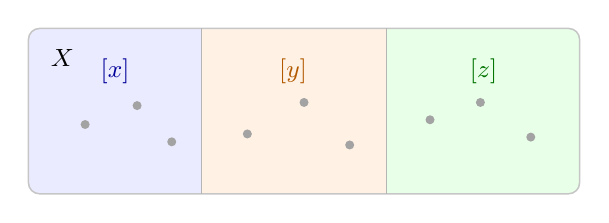
\begin{tikzpicture}[
  every node/.style={font=\small},
  ambient/.style={draw=gray!45, line width=0.55pt},
  seam/.style={draw=gray!58, line width=0.45pt},
  point/.style={circle, fill=gray!72, inner sep=1.15pt}
]
  \begin{scope}
    \clip[rounded corners=4pt] (0,0) rectangle (7.0,2.1);
    \fill[blue!8] (0,0) rectangle (2.2,2.1);
    \fill[orange!10] (2.2,0) rectangle (4.55,2.1);
    \fill[green!9] (4.55,0) rectangle (7.0,2.1);
  \end{scope}

  \draw[ambient, rounded corners=4pt] (0,0) rectangle (7.0,2.1);
  \draw[seam] (2.2,0) -- (2.2,2.1);
  \draw[seam] (4.55,0) -- (4.55,2.1);

  \node[anchor=north west] at (0.16,1.96) {$X$};
  \node[blue!60!black] at (1.10,1.55) {$[x]$};
  \node[orange!70!black] at (3.36,1.55) {$[y]$};
  \node[green!45!black] at (5.78,1.55) {$[z]$};

  \node[point] at (0.72,0.88) {};
  \node[point] at (1.38,1.12) {};
  \node[point] at (1.82,0.66) {};
  \node[point] at (2.78,0.76) {};
  \node[point] at (3.50,1.16) {};
  \node[point] at (4.08,0.62) {};
  \node[point] at (5.10,0.94) {};
  \node[point] at (5.74,1.16) {};
  \node[point] at (6.38,0.72) {};
\end{tikzpicture}

  \caption{Equivalence classes form disjoint blocks that cover the underlying set.}
  \label{fig:equivalence-classes-partition}
\end{illustrationfigure}

Figure \ref{fig:equivalence-classes-partition} depicts the partition in Proposition \ref{prop:equivalence-relations-partitions}. Every element of $X$ lies in one equivalence class, and distinct classes are disjoint.

\begin{proposition} \label{prop:partitions-determine-equivalence-relations} \hlt{Partitions Determine Equivalence Relations}\\
Let $X$ be a set and let $\mathcal{F}$ be a partition of $X$. For $x\in X$, let $B_x\in\mathcal{F}$ be the unique block containing $x$.\\
For $(x,y)\in X^2$, define $x\sim_{\mathcal{F}}y\Longleftrightarrow B_x=B_y$.
\begin{enumerate}[label=(\roman*)]
\setlength{\itemsep}{0pt}
\item \hlt{Equivalence relation}: $\sim_{\mathcal{F}}$ is an equivalence relation on $X$.
\item \hlt{Classes}: $(\forall x\in X)\,[x]_{\sim_{\mathcal{F}}}=B_x$, and $\{[x]_{\sim_{\mathcal{F}}}:x\in X\}=\mathcal{F}$.
\end{enumerate}
\begin{proof}
\begin{enumerate}[label=(\roman*)]
\setlength{\itemsep}{0pt}
\item For $x,y,z\in X$, $B_x=B_x$, so $x\sim_{\mathcal{F}}x$. If $x\sim_{\mathcal{F}}y$, then $B_x=B_y$, hence $B_y=B_x$ and $y\sim_{\mathcal{F}}x$.\\
Moreover, $(x\sim_{\mathcal{F}}y\land y\sim_{\mathcal{F}}z)\Rightarrow B_x=B_y=B_z\Rightarrow x\sim_{\mathcal{F}}z$. Thus $\sim_{\mathcal{F}}$ is reflexive, symmetric, and transitive.
\item Fix $x\in X$. If $y\in[x]_{\sim_{\mathcal{F}}}$, then $B_y=B_x$, so $y\in B_y=B_x$. If $y\in B_x$, then $B_x$ is a block containing $y$.\\
Uniqueness gives $B_y=B_x$, so $y\sim_{\mathcal{F}}x$ and $y\in[x]_{\sim_{\mathcal{F}}}$. Hence $[x]_{\sim_{\mathcal{F}}}=B_x$. Therefore $\{[x]_{\sim_{\mathcal{F}}}:x\in X\}\subseteq\mathcal{F}$.\\
If $B\in\mathcal{F}$, then $B\neq\emptyset$; choose $x\in B$. The uniqueness of $B_x$ gives $B=B_x=[x]_{\sim_{\mathcal{F}}}$, so the reverse containment holds.
\end{enumerate}
\hlt{Structural Commentary}: Block equality proves the axioms; uniqueness identifies classes with blocks.\\
\hlt{Key Insight}: Equivalent elements are assigned to the same block.
\end{proof}
\end{proposition}

\begin{example} \label{ex:rational-equivalence-classes-real-line} \hlt{Rational Equivalence on $\R$}\\
For $(x,y)\in\R^2$, define $x\sim_{\Q}y\Longleftrightarrow x-y\in\Q$. Fix $x,y,z\in\R$.
\begin{enumerate}[label=(\roman*)]
\setlength{\itemsep}{0pt}
\item \hlt{Reflexive}: $x-x=0\in\Q$.
\item \hlt{Symmetric}: $x-y\in\Q\Rightarrow y-x=-(x-y)\in\Q$.
\item \hlt{Transitive}: $(x-y\in\Q\land y-z\in\Q)\Rightarrow x-z=(x-y)+(y-z)\in\Q$.
\end{enumerate}
Thus $\sim_{\Q}$ is an equivalence relation, and $[x]_{\sim_{\Q}}=x+\Q=\{x+q:q\in\Q\}$.\\
A subset $\mathcal{R}\subseteq\R$ is a representative set iff $(\forall x\in\R)(\exists! r\in\mathcal{R})\,r\in x+\Q$.\\
\hlt{Key Insight}: Rational translation orbits are exactly the equivalence classes.
\end{example}

\begin{definition} \label{def:quotient-set-by-equivalence-relation} \hlt{Quotient Set}\\
Let $X$ be a set and let $\sim$ be an equivalence relation on $X$. The \hlt{quotient set} of $X$ by $\sim$ is $X/{\sim}\defeq\{[x]_{\sim}:x\in X\}$.
\end{definition}

\begin{proposition} \label{prop:quotient-map-well-defined-by-invariance} \hlt{Maps Defined on Equivalence Classes}\\
Let $X,Y$ be sets, let $\sim$ be an equivalence relation on $X$, and let $f:X\to Y$.\\
The assignment $g([x]_{\sim})\defeq f(x)$ defines $g:X/{\sim}\to Y$ iff $(\forall x,y\in X)\,[x\sim y\Rightarrow f(x)=f(y)]$.
\begin{proof}
\begin{enumerate}[label=(\roman*)]
\setlength{\itemsep}{0pt}
\item[$(\Rightarrow)$] Suppose $g$ is well-defined, $x\sim y$. Then $x\in[x]_{\sim}\cap[y]_{\sim}$, so $[x]_{\sim}=[y]_{\sim}$ by Proposition \ref{prop:equivalence-relations-partitions}. Thus $f(x)=g([x]_{\sim})=g([y]_{\sim})=f(y)$.
\item[$(\Leftarrow)$] Suppose $(\forall x,y\in X)\,[x\sim y\Rightarrow f(x)=f(y)]$. If $[x]_{\sim}=[y]_{\sim}$, then $x\in[y]_{\sim}$, whence $x\sim y$ and $f(x)=f(y)$.\\
Thus the assignment is independent of the representative. Hence it defines a map $g:X/{\sim}\to Y$.
\end{enumerate}
\hlt{Structural Commentary}: Equal classes prove necessity; representative independence proves sufficiency.\\
\hlt{Key Insight}: A class function cannot distinguish equivalent representatives.
\end{proof}
\end{proposition}


\subsection{Ordered Sets, Well-Orders, and Lattices}

\begin{definition} \label{def:ordered-set-vocabulary} \hlt{Ordered Set Vocabulary}\\
Let $S$ be a set, let $E,C\subseteq S$, and let $\leq_S\subseteq S^2$. Set $x<_Sy\Longleftrightarrow(x\leq_Sy\land x\neq y)$.\\
The relation $\leq_S$ is \hlt{antisymmetric} iff $(\forall x,y\in S)\,[(x\leq_Sy\land y\leq_Sx)\Rightarrow x=y]$. Elements $x,y\in S$ are \hlt{comparable} iff $x\leq_Sy\lor y\leq_Sx$.
\begin{enumerate}[label=(\roman*)]
\setlength{\itemsep}{0pt}
\item \hlt{Partial order}: The relation $\leq_S$ is a partial order iff it is reflexive, antisymmetric, and transitive. Then $(S,\leq_S)$ is a \hlt{poset}.
\item \hlt{Total order}: A partial order $\leq_S$ is total iff $(\forall x,y\in S)\,(x\leq_Sy\lor y\leq_Sx)$. Then $(S,\leq_S)$ is an \hlt{ordered set}.
\item \hlt{Chain}: If $\leq_S$ is a partial order, then $C$ is a chain iff $(\forall x,y\in C)\,(x\leq_Sy\lor y\leq_Sx)$.
\item \hlt{Well-order}: The order $\leq_S$ well-orders $S$ iff it is total and the following condition holds. $(\forall Y\in\mathcal{P}(S)\setminus\{\emptyset\})(\exists \ell\in Y)(\forall y\in Y)\,\ell\leq_Sy$.
\item \hlt{Bounds}: An element $\beta\in S$ is an upper bound of $E$ iff $(\forall x\in E)\,x\leq_S\beta$. It is a lower bound iff $(\forall x\in E)\,\beta\leq_Sx$.
\item \hlt{Boundedness}: The set $E$ is bounded above iff $(\exists \beta\in S)(\forall x\in E)\,x\leq_S\beta$. It is bounded below iff $(\exists \beta\in S)(\forall x\in E)\,\beta\leq_Sx$.
\item \hlt{Supremum}: For $\alpha\in S$, $\alpha=\sup E$ iff the following two conditions hold.
\begin{enumerate}[label=\arabic*.]
\setlength{\itemsep}{0pt}
\item \hlt{Upper bound}: $(\forall x\in E)\,x\leq_S\alpha$.
\item \hlt{Upper bound}: $(\forall x\in E)\,x\leq_S\alpha$.
\item \hlt{Least}: $(\forall \beta\in S)\,[((\forall x\in E)\,x\leq_S\beta)\Rightarrow\alpha\leq_S\beta]$.
\end{enumerate}
\item \hlt{Infimum}: For $\gamma\in S$, $\gamma=\inf E$ iff the following two conditions hold.
\begin{enumerate}[label=\arabic*.]
\setlength{\itemsep}{0pt}
\item \hlt{Lower bound}: $(\forall x\in E)\,\gamma\leq_Sx$.
\item \hlt{Greatest}: $(\forall \beta\in S)\,[((\forall x\in E)\,\beta\leq_Sx)\Rightarrow\beta\leq_S\gamma]$.
\end{enumerate}
\item \hlt{Maximal and minimal elements}: An element $m\in E$ is maximal iff $(\nexists x\in E)\,m<_Sx$. It is minimal iff $(\nexists x\in E)\,x<_Sm$.
\item \hlt{Least-upper-bound property}: This property is characterized by the following condition.\\
$(\forall A\in\mathcal{P}(S)\setminus\{\emptyset\})\,[((\exists \beta\in S)(\forall x\in A)\,x\leq_S\beta)\Rightarrow(\exists \alpha\in S)\,\alpha=\sup A]$.
\end{enumerate}
\end{definition}

\begin{illustrationfigure}[H]
  \centering
  \begin{tikzpicture}[
  x=0.80cm,
  y=0.82cm,
  >=Stealth,
  every node/.style={font=\small},
  axis/.style={gray!70, line width=0.55pt},
  setbar/.style={blue!70!black, line width=2.3pt, line cap=round},
  bound/.style={gray!50, line width=0.5pt},
  setpoint/.style={circle, fill=blue!70!black, inner sep=1.25pt},
  arrow/.style={->, gray!65, line width=0.5pt}
]
  \draw[axis] (-4.7,0) -- (4.7,0);

  \draw[setbar] (-1.35,0) -- (1.55,0);
  \foreach \x in {-0.75,-0.25,0.3,0.8,1.2} {
    \node[setpoint] at (\x,0) {};
  }

  \draw[arrow] (-1.35,0.60) -- (-1.35,0.16);
  \draw[arrow] (1.55,0.60) -- (1.55,0.16);
  \node[above] at (-1.35,0.60) {$\inf A$};
  \node[above] at (1.55,0.60) {$\sup A$};
  \node[below, yshift=-5pt] at (0.1,0) {$A$};

  \draw[bound] (-4.05,-0.42) -- (-4.05,-0.24) -- (-1.35,-0.24) -- (-1.35,-0.42);
  \node[below] at (-2.7,-0.42) {lower bounds};

  \draw[bound] (1.55,-0.42) -- (1.55,-0.24) -- (4.05,-0.24) -- (4.05,-0.42);
  \node[below] at (2.82,-0.42) {upper bounds};
\end{tikzpicture}

  \caption{The supremum is the least upper bound, while the infimum is the greatest lower bound.}
  \label{fig:supremum-infimum-bounds}
\end{illustrationfigure}

Figure \ref{fig:supremum-infimum-bounds} illustrates the bounds in Definition \ref{def:ordered-set-vocabulary} for a set $A$.\\
It marks $\inf A$ and $\sup A$ as extremal bounds; Example \ref{ex:supremum-need-not-be-attained} shows that neither need belong to the set.

\begin{example} \label{ex:supremum-need-not-be-attained} \hlt{Suprema Need Not Be Elements}\\
In $\Q$, set $E_1\defeq\{r\in\Q:r<0\}$ and $E_2\defeq\{r\in\Q:r\leq0\}$. Both sets have supremum $0$, but $0\notin E_1$ and $0\in E_2$.\\
For $E\defeq\{\frac{1}{n}:n\in\N\}$, $\sup E=1\in E$ and $\inf E=0\notin E$.\\
\hlt{Key Insight}: An extremal bound need not be an element of the set.
\end{example}

\begin{theorem} \label{thm:lub-property-gives-glb-property} \hlt{Least Upper Bounds Give Greatest Lower Bounds}\\
Let $(S,\leq)$ be an ordered set with the least-upper-bound property. Let $B\subseteq S$ be nonempty and bounded below. Then $\inf B$ exists in $S$.
\begin{proof} Set $L\defeq\{\ell\in S:(\forall b\in B)\,\ell\leq b\}$. $L\neq\emptyset$ by the boundedness of $B$ below. Choose $b_0\in B$.\\
Then $(\forall \ell\in L)\,\ell\leq b_0$, so $L$ is bounded above. Set $\alpha\defeq\sup L$; it exists in $S$ by the least-upper-bound property.\\
For $b\in B$, the element $b$ is an upper bound of $L$, so $\alpha\leq b$. Hence $\alpha\in L$. Moreover, $(\forall \ell\in L)\,\ell\leq\alpha$ by $\alpha=\sup L$.\\
Thus $\alpha$ is the greatest lower bound of $B$, and $\alpha=\inf B$.\\
\hlt{Structural Commentary}: The proof takes the supremum of the lower-bound set.\\
\hlt{Key Insight}: A nonempty set bounds its lower bounds above.
\end{proof}
\end{theorem}

\begin{definition} \label{def:lattice-vocabulary} \hlt{Lattice Vocabulary}\\
Let $(L,\leq)$ be a partially ordered set.
\begin{enumerate}[label=(\roman*)]
\setlength{\itemsep}{0pt}
\item \hlt{Meet}: For $x,y\in L$, the meet is $x\wedge y\defeq\inf\{x,y\}$ when this infimum exists.
\item \hlt{Join}: For $x,y\in L$, the join is $x\vee y\defeq\sup\{x,y\}$ when this supremum exists.
\item \hlt{Lattice}: The partially ordered set $L$ is a lattice iff the following condition holds. $(\forall x,y\in L)\,[x\wedge y\in L\land x\vee y\in L]$.
\item \hlt{Complete lattice}: A lattice $L$ is complete iff $(\forall E\subseteq L)\,[\inf E\in L\land\sup E\in L]$.
\item \hlt{Bottom}: An element $\bot\in L$ is a bottom element iff $(\forall x\in L)\,\bot\leq x$.
\item \hlt{Top}: An element $\top\in L$ is a top element iff $(\forall x\in L)\,x\leq\top$.
\item \hlt{Modular lattice}: A lattice $L$ is modular iff the following law holds. $(\forall x,y,z\in L)\,[x\leq z\Rightarrow z\wedge(y\vee x)=(z\wedge y)\vee x]$.
\end{enumerate}
\end{definition}


\subsection{Relations Between Sets and Closures}

\begin{definition} \label{def:inverse-and-composition-of-relations} \hlt{Inverse and Composition of Relations}\\
Let $X,Y,Z$ be sets, let $R\subseteq X\times Y$, and let $S\subseteq Y\times Z$.
\begin{enumerate}[label=(\roman*)]
\setlength{\itemsep}{0pt}
\item \hlt{Inverse}: $R^{-1}\defeq\{(y,x)\in Y\times X:(x,y)\in R\}$.
\item \hlt{Composition}: $S\circ R\defeq\{(x,z)\in X\times Z:(\exists y\in Y)\,[(x,y)\in R\land(y,z)\in S]\}$.
\item \hlt{Diagonal}: $\Delta_X\defeq\{(x,x):x\in X\}$.
\end{enumerate}
\end{definition}

\begin{proposition} \label{prop:inverse-and-composition-laws} \hlt{Inverse and Composition Laws}\\
Let $W,X,Y,Z$ be sets. Let $R\subseteq X\times Y$, let $S\subseteq Y\times Z$, and let $T\subseteq Z\times W$.
\begin{enumerate}[label=(\roman*)]
\setlength{\itemsep}{0pt}
\item \hlt{Identity}: $\Delta_Y\circ R=R=R\circ\Delta_X$.
\item \hlt{Associativity}: $T\circ(S\circ R)=(T\circ S)\circ R$.
\item \hlt{Involution}: $(R^{-1})^{-1}=R$.
\item \hlt{Reversal}: $(S\circ R)^{-1}=R^{-1}\circ S^{-1}$.
\end{enumerate}
\begin{proof}
\begin{enumerate}[label=(\roman*)]
\setlength{\itemsep}{0pt}
\item[$(i)$] For $(x,y)\in X\times Y$, $(x,y)\in\Delta_Y\circ R\Longleftrightarrow(\exists u\in Y)\,[(x,u)\in R\land u=y]\Longleftrightarrow(x,y)\in R$.\\
For the right identity, $(x,y)\in R\circ\Delta_X\Longleftrightarrow(\exists v\in X)\,[v=x\land(v,y)\in R]\Longleftrightarrow(x,y)\in R$.
\item[$(ii)$]$(\Rightarrow)$ Suppose $(x,w)\in T\circ(S\circ R)$. Choose $z\in Z$ with $(x,z)\in S\circ R$ and $(z,w)\in T$.\\
Choose $y\in Y$ with $(x,y)\in R$ and $(y,z)\in S$. Thus $(y,w)\in T\circ S$ and $(x,w)\in(T\circ S)\circ R$.
\item[$(ii)$]$(\Leftarrow)$ Suppose $(x,w)\in(T\circ S)\circ R$. Choose $y\in Y$ with $(x,y)\in R$ and $(y,w)\in T\circ S$.\\
Choose $z\in Z$ with $(y,z)\in S$ and $(z,w)\in T$. Thus $(x,z)\in S\circ R$ and $(x,w)\in T\circ(S\circ R)$.
\item[$(iii)$] For $(x,y)\in X\times Y$, $(x,y)\in(R^{-1})^{-1}\Longleftrightarrow(y,x)\in R^{-1}\Longleftrightarrow(x,y)\in R$.
\item[$(iv)$]$(\Rightarrow)$ Suppose $(z,x)\in(S\circ R)^{-1}$. Then $(x,z)\in S\circ R$.\\
Choose $y\in Y$ with $(x,y)\in R$ and $(y,z)\in S$. Hence $(z,y)\in S^{-1}$ and $(y,x)\in R^{-1}$, so $(z,x)\in R^{-1}\circ S^{-1}$.
\item[$(iv)$]$(\Leftarrow)$ Suppose $(z,x)\in R^{-1}\circ S^{-1}$. Choose $y\in Y$ with $(z,y)\in S^{-1}$ and $(y,x)\in R^{-1}$.\\
Then $(y,z)\in S$ and $(x,y)\in R$, so $(x,z)\in S\circ R$ and $(z,x)\in(S\circ R)^{-1}$.
\end{enumerate}
\hlt{Structural Commentary}: Membership expansion and witness comparison prove the four laws.\\
\hlt{Key Insight}: Composition records witnesses; inversion reverses their order.
\end{proof}
\end{proposition}

\begin{definition} \label{def:relation-powers-and-closures} \hlt{Relation Powers and Closures}\\
Let $X$ be a set and let $R\subseteq X^2$. Set $R^0\defeq\Delta_X$ and $R^{n+1}\defeq R\circ R^n$ for $n\in\N_0$.
\begin{enumerate}[label=(\roman*)]
\setlength{\itemsep}{0pt}
\item \hlt{Reflexive closure}: $\operatorname{Ref}(R)\defeq R\cup\Delta_X$.
\item \hlt{Transitive closure}: $R^+\defeq\bigcup\limits_{n\in\N}R^n$.
\item \hlt{Reflexive-transitive closure}: $R^*\defeq\bigcup\limits_{n\in\N_0}R^n=\Delta_X\cup R^+$.
\end{enumerate}
\end{definition}

\begin{lemma} \label{lem:addition-law-for-relation-powers} \hlt{Addition Law for Relation Powers}\\
Let $X$ be a set and let $R\subseteq X^2$. Then $(\forall m,n\in\N_0)\,R^n\circ R^m=R^{m+n}$.
\begin{proof} Fix $m\in\N_0$. For $r\in\N$, let $P_r$ assert $R^{r-1}\circ R^m=R^{m+r-1}$.\\
The identity $R^0\circ R^m=\Delta_X\circ R^m=R^m$ holds by Proposition \ref{prop:inverse-and-composition-laws}(i), so $P_1$ holds.\\
Assume $P_r$. Then $R^r\circ R^m=R\circ(R^{r-1}\circ R^m)$ by Proposition \ref{prop:inverse-and-composition-laws}(ii) and the recursion.\\
Hence $R^r\circ R^m=R\circ R^{m+r-1}=R^{m+r}$ by $P_r$ and the recursion, so $P_{r+1}$ holds.\\
Consequently, $(\forall r\in\N)\,P_r$ by induction. For $n\in\N_0$, take $r=n+1$ to obtain $R^n\circ R^m=R^{m+n}$.\\
\hlt{Structural Commentary}: Reindexed induction combines the recursive power law with associativity.\\
\hlt{Key Insight}: Relation composition adds power indices.
\end{proof}
\end{lemma}

\begin{theorem} \label{thm:reflexive-and-transitive-closures-are-smallest} \hlt{Minimality of Reflexive and Transitive Closures}\\
Let $X$ be a set and let $R\subseteq X^2$.
\begin{enumerate}[label=(\roman*)]
\setlength{\itemsep}{0pt}
\item \hlt{Reflexive}: $\operatorname{Ref}(R)$ is the smallest reflexive relation on $X$ containing $R$.
\item \hlt{Transitive}: $R^+$ is the smallest transitive relation on $X$ containing $R$.
\item \hlt{Reflexive and transitive}: $R^*$ is the smallest reflexive and transitive relation on $X$ containing $R$.
\end{enumerate}
\begin{proof}
\begin{enumerate}[label=(\roman*)]
\setlength{\itemsep}{0pt}
\item The relation $\operatorname{Ref}(R)$ contains $R$ and $\Delta_X$, so it is reflexive.\\
If $Q\subseteq X^2$ is reflexive and $R\subseteq Q$, then $\Delta_X\subseteq Q$, whence $\operatorname{Ref}(R)=R\cup\Delta_X\subseteq Q$.
\item Since $R=R^1$, $R\subseteq R^+$. Suppose $(x,y)\in R^+$ and $(y,z)\in R^+$. Choose $m,n\in\N$ with $(x,y)\in R^m$ and $(y,z)\in R^n$.\\
Then $(x,z)\in R^{m+n}\subseteq R^+$ by Lemma \ref{lem:addition-law-for-relation-powers}, so $R^+$ is transitive. Let $Q\subseteq X^2$ be transitive with $R\subseteq Q$.\\
For $n\in\N$, let $P_n$ assert $R^n\subseteq Q$. $P_1$ holds by $R^1=R\subseteq Q$. Assume $P_n$. Then $R^{n+1}=R\circ R^n\subseteq Q\circ Q$ by $R\subseteq Q$ and $P_n$.\\
Also $Q\circ Q\subseteq Q$ by the transitivity of $Q$, so $P_{n+1}$ holds. Thus $(\forall n\in\N)\,P_n$ by induction, and $R^+\subseteq Q$.
\item The relation $R^*$ contains $R$ and is reflexive by $R^*=\Delta_X\cup R^+$. Suppose $(x,y)\in R^*$ and $(y,z)\in R^*$.\\
Choose $m,n\in\N_0$ with $(x,y)\in R^m$ and $(y,z)\in R^n$. Then $(x,z)\in R^{m+n}\subseteq R^*$ by Lemma \ref{lem:addition-law-for-relation-powers}, so $R^*$ is transitive.\\
If $Q\subseteq X^2$ is reflexive and transitive with $R\subseteq Q$, then $\Delta_X\subseteq Q$ and $R^+\subseteq Q$ by (ii). Thus $R^*=\Delta_X\cup R^+\subseteq Q$.
\end{enumerate}
\hlt{Structural Commentary}: Containment, closure, and minimality are verified in parallel.\\
\hlt{Key Insight}: Closure is generated by diagonal pairs together with finite composites.
\end{proof}
\end{theorem}

\begin{example} \label{ex:successor-relation-closures} \hlt{Closures of the Successor Relation}\\
Define $R\subseteq\Z^2$ by $m\,R\,n\Longleftrightarrow n=m+1$. For $k\in\N$, let $P_k$ assert $(\forall m,n\in\Z)\,[m\,R^k\,n\Longleftrightarrow n=m+k]$. $P_1$ holds by the definition of $R$.\\
Assume $P_k$. For $(m,n)\in\Z^2$, $m\,R^{k+1}\,n\Longleftrightarrow(\exists u\in\Z)\,[u=m+k\land n=u+1]\Longleftrightarrow n=m+k+1$.\\
Thus $P_{k+1}$ holds, and $(\forall k\in\N)\,P_k$ by induction.
\begin{enumerate}[label=(\roman*)]
\setlength{\itemsep}{0pt}
\item $\operatorname{Ref}(R)=\{(m,n)\in\Z^2:n=m\lor n=m+1\}$.
\item $R^+=\{(m,n)\in\Z^2:m<n\}$.
\item $R^*=\{(m,n)\in\Z^2:m\leq n\}$.
\end{enumerate}
\hlt{Key Insight}: Finite successor compositions generate the strict and nonstrict integer orders.
\end{example}

\begin{definition} \label{def:order-isomorphism} \hlt{Order Isomorphism}\\
Let $(S,\leq_S)$ and $(T,\leq_T)$ be partially ordered sets.\\
A bijection $f:S\to T$ is an \hlt{order isomorphism} when the following condition holds. $(\forall x,y\in S)\,[x\leq_Sy\Longleftrightarrow f(x)\leq_Tf(y)]$.\\
The two partially ordered sets are \hlt{order-isomorphic} when such a map exists.
\end{definition}

\begin{example} \label{ex:basic-order-isomorphisms} \hlt{Basic Order Isomorphisms}
\begin{enumerate}[label=(\roman*)]
\setlength{\itemsep}{0pt}
\item Define $f:\Z\to\{2n:n\in\Z\}$ by $f(n)\defeq2n$. Its inverse is $2n\mapsto n$, so $f$ is bijective.\\
Moreover, $m\leq n\Longleftrightarrow2m\leq2n$; hence $f$ is an order isomorphism for the usual orders.
\item Let $X$ be a set and define $c:\mathcal{P}(X)\to\mathcal{P}(X)$ by $c(A)\defeq X\setminus A$. Since $c(c(A))=A$, the map is bijective.\\
Moreover, $A\subseteq B\Longleftrightarrow c(A)\supseteq c(B)$. Hence $c$ is an order isomorphism from $(\mathcal{P}(X),\subseteq)$ to $(\mathcal{P}(X),\supseteq)$.
\item Let $(S,\leq)$ be a poset and set $\downarrow s\defeq\{x\in S:x\leq s\}$. Define $\eta:S\to\{\downarrow s:s\in S\}$ by $\eta(s)\defeq\downarrow s$.\\
If $s\leq t$, then $\downarrow s\subseteq\downarrow t$ by transitivity. If $\downarrow s\subseteq\downarrow t$, then $s\in\downarrow s\subseteq\downarrow t$, so $s\leq t$. Thus $s\leq t\Longleftrightarrow\eta(s)\subseteq\eta(t)$.\\
If $\eta(s)=\eta(t)$, then $s\leq t$ and $t\leq s$, so $s=t$ by antisymmetry. Thus $\eta$ is injective.\\
It is surjective by the definition of its codomain, so it is an order isomorphism.
\end{enumerate}
\hlt{Key Insight}: Order isomorphisms preserve comparisons while changing their representation.
\end{example}


\section{Cardinality, Choice, and Infinite Sets}

Choice and maximality principles come first as foundational tools; cardinality then compares sets by functions rather than by informal size.

\subsection{Choice and Zorn's Lemma}

\begin{definition} \label{def:choice-function} \hlt{Choice Function}\\
Let $\mathcal{F}$ be a family of nonempty sets, let $I$ be a set, and let $(X_i)_{i\in I}$ be an indexed family of nonempty sets.
\begin{enumerate}[label=(\roman*)]
\setlength{\itemsep}{0pt}
\item A \hlt{choice function} on $\mathcal{F}$ is a map $c:\mathcal{F}\to\bigcup\limits_{F\in\mathcal{F}}F$ satisfying $(\forall F\in\mathcal{F})\,c(F)\in F$.
\item An \hlt{indexed choice function} for $(X_i)_{i\in I}$ is a map $c:I\to\bigcup\limits_{i\in I}X_i$ satisfying $(\forall i\in I)\,c(i)\in X_i$.
\end{enumerate}
\end{definition}

\begin{principle} \label{princ:axiom-of-choice-analysis} \hlt{Choice Principle}\\
Let $I$ be a set and let $(X_i)_{i\in I}$ be an indexed family of nonempty sets. The axiom of choice asserts $(\exists c:I\to\bigcup\limits_{i\in I}X_i)(\forall i\in I)\,c(i)\in X_i$.\\
Equivalently, $\prod\limits_{i\in I}X_i\neq\varnothing$. An explicit $c$ proves existence directly; the principle supplies simultaneous choices without an explicit rule.
\end{principle}

\begin{principle} \label{princ:zorns-lemma} \hlt{Zorn's Lemma}\\
Let $(P,\leq)$ be a poset with $P\neq\varnothing$. Assume the following chain-upper-bound condition.\\
$(\forall C\subseteq P)\,[((\forall x,y\in C)\,(x\leq y\lor y\leq x))\Rightarrow(\exists u\in P)(\forall c\in C)\,c\leq u]$. Then $(\exists m\in P)(\forall x\in P)\,(m\leq x\Rightarrow x=m)$.
\end{principle}

\begin{definition} \label{def:inclusion-and-containment-orders-for-zorn} \hlt{Inclusion and Containment Orders}\\
Let $\mathcal{F}$ be a family of sets and let $\mathcal{A}\subseteq\mathcal{F}$.
\begin{enumerate}[label=(\roman*)]
\setlength{\itemsep}{0pt}
\item \hlt{Inclusion}: for $A,B\in\mathcal{F}$, define $A\leq B$ iff $A\subseteq B$. An upper bound of $\mathcal{A}$ is $U\in\mathcal{F}$ satisfying $(\forall A\in\mathcal{A})\,A\subseteq U$.\\
An element $M\in\mathcal{F}$ is maximal iff $(\forall B\in\mathcal{F})\,(M\subseteq B\Rightarrow B=M)$.
\item \hlt{Reverse inclusion}: for $A,B\in\mathcal{F}$, define $A\leq B$ iff $B\subseteq A$. An upper bound of $\mathcal{A}$ is $U\in\mathcal{F}$ satisfying $(\forall A\in\mathcal{A})\,U\subseteq A$.\\
An element $M\in\mathcal{F}$ is maximal iff $(\forall B\in\mathcal{F})\,(B\subseteq M\Rightarrow B=M)$.
\end{enumerate}
\end{definition}

\begin{proposition} \label{prop:inclusion-and-reverse-inclusion-partial-orders} \hlt{Inclusion Orders Are Partial Orders}\\
Let $\mathcal{F}$ be a family of sets. Inclusion and reverse inclusion are partial orders on $\mathcal{F}$.
\begin{proof}
Fix $A,B,C\in\mathcal{F}$. Since $A\subseteq A$, inclusion is reflexive. If $A\subseteq B$ and $B\subseteq C$, then $A\subseteq C$, so inclusion is transitive.\\
If $A\subseteq B$ and $B\subseteq A$, then $A=B$ by Assumption \ref{assump:set-extensionality}, so inclusion is antisymmetric. Hence inclusion is a partial order.\\
For reverse inclusion, $A\supseteq A$ gives reflexivity, $A\supseteq B\supseteq C$ gives $A\supseteq C$, and $A\supseteq B\supseteq A$ gives $A=B$ by Assumption \ref{assump:set-extensionality}.\\
Thus reverse inclusion is also a partial order.\\
\hlt{Structural Commentary}: Each order law follows from the corresponding containment law and set extensionality.\\
\hlt{Key Insight}: Reversing containment preserves reflexivity, transitivity, and antisymmetry.
\end{proof}
\end{proposition}

\begin{proofmethod} \label{meth:zorn-maximality-template} \hlt{Zorn Maximality Template}\\
Use this method when the target follows from a candidate admitting no proper admissible extension.\\
Let $P$ be the set of candidates, and let $\leq$ record admissible extension.
\begin{enumerate}[label=(\roman*)]
\setlength{\itemsep}{0pt}
\item Verify that $P\neq\varnothing$ and that $\leq$ is a partial order on $P$.
\item Fix a chain $C\subseteq P$, construct $u\in P$, and prove $(\forall p\in C)\,p\leq u$.
\item Obtain a maximal $m\in P$ by Principle \ref{princ:zorns-lemma}, and prove that maximality forces the target property.
\end{enumerate}
For $C\neq\varnothing$, common candidates are $\bigcup\limits_{A\in C}A$ under inclusion and $\bigcap\limits_{A\in C}A$ under reverse inclusion.\\
Under reverse inclusion, another object contained in every member of $C$ may be necessary.\\
If $C=\varnothing$, any element of $P$ is an upper bound. In every case, prove $u\in P$; this is the indispensable admissibility check.\\
\hlt{Key Idea}: A chain bound must preserve every admissibility condition defining the candidate set.
\end{proofmethod}


\subsection{Same Cardinality, Finite, Countable, and Uncountable}

\begin{definition} \label{def:cardinality-equivalence} \hlt{Same Cardinality}\\
For sets $A,B$, define $A\sim_{\#}B$ iff there exists a bijection $f:A\to B$.\\
Then $A$ and $B$ have \hlt{same cardinality}, or are \hlt{equivalent}. The relation $\sim_{\#}$ is an equivalence relation.\\
$\operatorname{id}_A$ proves reflexivity, inverses of bijections prove symmetry, and composition of bijections proves transitivity.
\end{definition}

\begin{definition} \label{def:finite-countable-uncountable} \hlt{Finite, Countable, and Uncountable}\\
Set $J_0\defeq\emptyset$, and for $n\geq1$ set $J_n\defeq\{1,2,\ldots,n\}$. A set $A$ is
\begin{enumerate}[label=(\roman*)]
\setlength{\itemsep}{0pt}
\item \hlt{finite} if $A\sim_{\#} J_n$ for some $n\in\N$;
\item \hlt{infinite} if it is not finite;
\item \hlt{countable} if $A\sim_{\#} \N$;
\item \hlt{uncountable} if it is neither finite nor countable;
\item \hlt{at most countable} if it is finite or countable.
\end{enumerate}
Countable sets are also called enumerable or denumerable.
\end{definition}

\begin{proposition} \label{prop:finite-cardinality-well-defined} \hlt{Finite Cardinality is Well Defined}\\
Let $m,n\in\N$. If $A\sim_{\#}J_m$ and $A\sim_{\#}J_n$, then $m=n$.\\
Hence for finite $A$, the value $\#A\defeq n$ with $A\sim_{\#}J_n$ is well-defined.
\begin{proof} By transitivity of $\sim_{\#}$, it suffices to prove $J_m\sim_{\#}J_n\Rightarrow m=n$.\\
Induct on $m$. If $m=0$, then $J_m=\emptyset$, so any bijection $J_m\to J_n$ forces $J_n=\emptyset$ and $n=0$.\\
Assume the claim for $m-1$, with $m\geq1$, and let $f:J_m\to J_n$ be bijective. Then $n\geq1$.\\
Removing $m$ and $f(m)$ gives a bijection $J_m\setminus\{m\}\to J_n\setminus\{f(m)\}$. Since these sets have the standard relabelings $J_{m-1}$ and $J_{n-1}$, the induction hypothesis gives $m-1=n-1$, hence $m=n$.\\
\hlt{Structural Commentary}: Finite size is bijection-invariant.\\
\hlt{Key Insight}: Remove one matched element.
\end{proof}
\end{proposition}

\begin{definition} \label{def:finite-set-summation} \hlt{Summation over a Finite Set}\\
Let $X$ be a finite set with $\#X=n$, and let $f:X\to\C$.\\
Choose any bijection $g:J_n\to X$, where $J_n=\{1,\ldots,n\}$, and set $\sum\limits_{x\in X}f(x)\defeq\sum_{i=1}^{n}f(g(i))$.\\
When $X=\emptyset$, this is the empty sum $0$.\\
\hlt{Key Insight}: Proposition \ref{prop:finite-set-summation-laws} shows that the value is independent of the chosen bijection.
\end{definition}

\begin{proposition} \label{prop:finite-set-summation-laws} \hlt{Finite Set Summation Laws}\\
Let $X,Y$ be finite sets.
\begin{enumerate}[label=(\roman*)]
\setlength{\itemsep}{0pt}
\item \hlt{Well-definedness}: different bijections $J_{\#X}\to X$ give the same value in Definition \ref{def:finite-set-summation}.
\item \hlt{Substitution}: if $h:Y\to X$ is a bijection and $f:X\to\C$, then $\sum\limits_{x\in X}f(x)=\sum\limits_{y\in Y}f(h(y))$.
\item \hlt{Linearity}: for $f,g:X\to\C$ and $c\in\C$, $\sum\limits_{x\in X}(f(x)+g(x))=\sum\limits_{x\in X}f(x)+\sum\limits_{x\in X}g(x)$ and $\sum\limits_{x\in X}cf(x)=c\sum\limits_{x\in X}f(x)$.
\item \hlt{Disjoint unions}: if $X\cap Y=\emptyset$ and $f:X\cup Y\to\C$, then $\sum\limits_{z\in X\cup Y}f(z)=\sum\limits_{x\in X}f(x)+\sum\limits_{y\in Y}f(y)$.
\item \hlt{Finite Fubini}: if $f:X\times Y\to\C$, then $\sum\limits_{x\in X}\sum\limits_{y\in Y}f(x,y)=\sum\limits_{(x,y)\in X\times Y}f(x,y)=\sum\limits_{y\in Y}\sum\limits_{x\in X}f(x,y)$.
\end{enumerate}
\begin{proof}
\begin{enumerate}[label=(\roman*)]
\setlength{\itemsep}{0pt}
\item For $f:X\to\C$, let $n=\#X$ and let $g,k:J_n\to X$ be bijections. Induct on $n$. The case $n=0$ is empty. If $n\geq1$, let $j\in J_n$ satisfy $k(j)=g(n)$. Removing $n$ from $g$ and $j$ from $k$ gives bijections onto $X\setminus\{g(n)\}$; after relabeling by $J_{n-1}$, the induction hypothesis makes the remaining sums equal. Adding the common last term $f(g(n))=f(k(j))$ gives equality of the two sums.
\item Let $g:J_{\#Y}\to Y$ be a bijection. Then $h\circ g:J_{\#Y}\to X$ is a bijection, so $\#Y=\#X$ by Proposition \ref{prop:finite-cardinality-well-defined}.\\
Hence, by (i) and Definition \ref{def:finite-set-summation}, $\sum\limits_{x\in X}f(x)=\sum\limits_{i=1}^{\#Y}f(h(g(i)))=\sum\limits_{y\in Y}f(h(y))$.
\item Choose a bijection $\gamma:J_{\#X}\to X$.\\
Proposition \ref{prop:finite-sum-basic-laws} gives $\sum\limits_{x\in X}(f(x)+g(x)) =\sum\limits_{x\in X}f(x)+\sum\limits_{x\in X}g(x)$ and $\sum\limits_{x\in X}cf(x)=c\sum\limits_{x\in X}f(x)$
\item Let $\alpha:J_{\#X}\to X$ and $\beta:J_{\#Y}\to Y$ be bijections, and enumerate $X\cup Y$ by listing $\alpha$ first and then $\beta$. Since $X\cap Y=\emptyset$, this is a bijection, and Proposition \ref{prop:finite-sum-basic-laws} gives $\sum\limits_{z\in X\cup Y}f(z)=\sum\limits_{x\in X}f(x)+\sum\limits_{y\in Y}f(y)$.
\item Let $\alpha:J_{\#X}\to X$ and $\beta:J_{\#Y}\to Y$ be bijections.\\
The maps $\ell((i-1)\#Y+j)=(\alpha(i),\beta(j))$ and $r((j-1)\#X+i)=(\alpha(i),\beta(j))$ for $i\in J_{\#X}$ and $j\in J_{\#Y}$ give the two lexicographic bijections $J_{(\#X)(\#Y)}\to X\times Y$.\\
Applying Definition \ref{def:finite-set-summation}, Proposition \ref{prop:finite-sum-basic-laws}, and (i) yields $\sum\limits_{x\in X}\sum\limits_{y\in Y}f(x,y) =\sum\limits_{(x,y)\in X\times Y}f(x,y) =\sum\limits_{y\in Y}\sum\limits_{x\in X}f(x,y)$.
\end{enumerate}
\hlt{Structural Commentary}: A finite set sum is an order-free finite sum.\\
\hlt{Key Insight}: Bijections are bookkeeping devices; the value does not depend on the bookkeeping order.
\end{proof}
\end{proposition}

\begin{definition} \label{def:sequence-as-enumeration} \hlt{Sequences as Enumerations}\\
Let $A$ be a set.
\begin{enumerate}[label=(\roman*)]
\setlength{\itemsep}{0pt}
\item A \hlt{sequence} in $A$ is a map $x:\N\to A$, written $(x_n)_{n\in\N}$ with $x_n\defeq x(n)$.
\item A sequence $x:\N\to A$ \hlt{enumerates} $A$ iff $x(\N)=A$.
\item A sequence $x:\N\to A$ is a \hlt{distinct enumeration} of $A$ iff $x:\N\to A$ is bijective.
\end{enumerate}
Thus $A$ is countable iff it has a distinct enumeration.
\end{definition}

\begin{example} \label{ex:integers-are-countable} \hlt{The Integers Are Countable}\\
The set $\Z$ is countable. One explicit enumeration is given by
\begin{align}
f(n)=
\begin{cases}
\frac{n}{2}, & n \text{ even},\\[2mm]
-\frac{n-1}{2}, & n \text{ odd},
\end{cases}
\qquad n\in\N. \nonumber
\end{align}
This lists $\Z$ as $0,1,-1,2,-2,3,-3,\ldots$.
\end{example}

\begin{theorem} \label{thm:infinite-subset-of-countable-is-countable} \hlt{Infinite Subsets of Countable Sets}\\
Let $A$ be countable and let $E\subseteq A$ be infinite. Then $E$ is countable.
\begin{proof} Let $x:\N\to A$ be a distinct enumeration of $A$. Since $E$ is infinite, $I_E\defeq\{n\in\N:x_n\in E\}$ is infinite.\\
Write $I_E=\{n_1<n_2<\cdots\}$ and define $g:\N\to E$ by $g(k)\defeq x_{n_k}$. The terms $(x_n)$ are distinct, so $g$ is injective.\\
If $y\in E$, then $y=x_n$ for a unique $n\in\N$; since $n\in I_E$, $n=n_k$ for some $k$, and $y=g(k)$.\\
Thus $g$ is bijective, so $E$ is countable.\\
\hlt{Structural Commentary}: Subsets select indices.\\
\hlt{Key Insight}: Keep the hitting indices.
\end{proof}
\end{theorem}

\begin{proposition} \label{prop:subsets-and-images-at-most-countable} \hlt{Subsets and Images of At Most Countable Sets}\\
Let $A$ be at most countable.
\begin{enumerate}[label=(\roman*)]
\setlength{\itemsep}{0pt}
\item If $B\subseteq A$, then $B$ is at most countable.
\item If $f:A\to Y$ is a function, then $f(A)$ is at most countable.
\end{enumerate}
\begin{proof}
If $A$ is finite, both claims are immediate. Otherwise write $A=\{a_n:n\in\N\}$ with the $a_n$ distinct.
\begin{enumerate}[label=(\roman*)]
\setlength{\itemsep}{0pt}
\item If $B$ is infinite, let $I_B\defeq\{n:a_n\in B\}=\{n_1<n_2<\cdots\}$.\\
Then $k\mapsto a_{n_k}$ bijects $\N$ onto $B$; the finite case is trivial.
\item Let $I\defeq\{n:f(a_n)\notin\{f(a_m):m<n\}\}$. By (i), $I$ is at most countable, $n\mapsto f(a_n)$ bijects $I$ onto $f(A)$.
\end{enumerate}
\hlt{Structural Commentary}: Subsets select indices; images select first appearances.\\
\hlt{Key Insight}: Subsets and images preserve at-most-countability.
\end{proof}
\end{proposition}

\begin{proposition} \label{prop:at-most-countable-iff-enumerable-image} \hlt{At Most Countable Sets Are Exactly Enumerable Images}\\
For a set $B$, the following are equivalent:
\begin{enumerate}[label=(\roman*)]
\setlength{\itemsep}{0pt}
\item $B$ is at most countable.
\item $B=\emptyset$ or there exists a surjection $f:\N\to B$.
\end{enumerate}
Thus a nonempty set is at most countable iff it is the image of a sequence.
\begin{proof}
\begin{enumerate}[label=(\roman*)]
\setlength{\itemsep}{0pt}
\item[$(i)$]$\Rightarrow(ii)$ If $B=\emptyset$, (ii) holds. If $B$ is countable, choose a bijection $f:\N\to B$. If $B=\{b_1,\ldots,b_m\}$ is finite and nonempty, define $f(0)=b_1$, $f(n)=b_n$ for $1\leq n\leq m$, and $f(n)=b_m$ for $n>m$.\\
In both nonempty cases, $f:\N\to B$ is surjective.
\item[$(ii)$]$\Rightarrow(i)$ If $B=\emptyset$, then $B$ is finite.\\
If $f:\N\to B$ is surjective, then $B=f(\N)$ is at most countable by Proposition \ref{prop:subsets-and-images-at-most-countable}.
\end{enumerate}
\hlt{Structural Commentary}: Surjections list with repetition.\\
\hlt{Key Insight}: At most countable means sequence image.
\end{proof}
\end{proposition}

\begin{figure}[H]
  \centering
  \begin{tikzpicture}[
  >=Stealth,
  every node/.style={font=\small},
  entry/.style={draw=gray!55, fill=gray!5, rounded corners=1pt, minimum width=0.62cm, minimum height=0.40cm},
  active/.style={draw=orange!60!black, fill=orange!10},
  scan/.style={->, blue!70!black, line width=0.7pt},
  guide/.style={orange!75!black, line width=0.65pt},
  output/.style={draw=gray!55, fill=gray!5, rounded corners=1pt, inner xsep=5pt, inner ysep=4pt}
]
  \draw[guide] (1.70,-0.65) -- (0.85,-1.30);
  \draw[guide] (2.55,-0.65) -- (0.85,-1.95);
  \draw[guide] (3.40,-0.65) -- (0.85,-2.60);

  \foreach \row/\name in {1/E_1,2/E_2,3/E_3,4/E_4} {
    \node[anchor=east] at (0,-0.65*\row) {$\name$};
    \foreach \col in {1,...,5} {
      \node[entry] (x-\row-\col) at (0.85*\col,-0.65*\row) {$x_{\row\col}$};
    }
    \node[anchor=west, gray!65] at (4.55,-0.65*\row) {$\cdots$};
  }

  \foreach \row/\col in {1/1,1/2,2/1,1/3,2/2,3/1,1/4,2/3,3/2,4/1} {
    \node[entry, active] at (0.85*\col,-0.65*\row) {$x_{\row\col}$};
  }

  \node[output, anchor=west] (list) at (5.25,-1.45)
    {$x_{11},\,x_{12},\,x_{21},\,x_{13},\,x_{22},\,x_{31},\,x_{14},\,\cdots$};
  \draw[scan] (4.55,-1.45) -- (list.west);
\end{tikzpicture}

  \caption{Diagonal scan of countable rows into one sequence, skipping repeats.}
  \label{fig:countable-union-diagonal-scan}
\end{figure}

\begin{theorem} \label{thm:countable-union-of-countable-sets}\label{thm:cardinality-main-results-source-todo} \hlt{Countable Union of Countable Sets}\\
Let $(E_n)_{n\geq1}$ be countable sets and set $S\defeq\bigcup\limits_{n=1}^{\infty}E_n$. Then $S$ is countable.
\begin{proof} For each $n\geq1$, choose a bijection $x_n:\N\to E_n$ and write $x_{n,k}\defeq x_n(k)$.\\
Let $D\defeq\{(n,k):n\geq1,\ k\in\N\}$. Diagonal order gives a surjection $d:\N\to D$.\\
Set $a(t)\defeq x_{n,k}$ for $d(t)=(n,k)$; then $a(\N)=S$, so $S$ is at most countable by Proposition \ref{prop:at-most-countable-iff-enumerable-image}.\\
Since $E_1\subseteq S$ and $E_1$ is countable, $S$ is infinite. Hence $S$ is countable.\\
\hlt{Structural Commentary}: Diagonal scanning enumerates pairs.\\
\hlt{Key Insight}: Scan the two-index list.
\end{proof}
\end{theorem}

\begin{corollary} \label{cor:at-most-countable-union-at-most-countable} \hlt{At Most Countable Unions}\\
If $A$ is at most countable and $B_\alpha$ is at most countable for each $\alpha\in A$, then $\bigcup\limits_{\alpha\in A}B_\alpha$ is at most countable.
\begin{proof} Let $T\defeq\bigcup\limits_{\alpha\in A}B_\alpha$. If $T=\emptyset$, we are done.\\
Otherwise write the nonempty $B_\alpha$ as $(B_{\alpha_j})_{j\geq1}$, with repetitions if needed, and enumerate $B_{\alpha_j}$ by $(b_{jk})_{k\in\N}$.\\
A diagonal scan of $(b_{jk})$ has image $T$, so Proposition \ref{prop:subsets-and-images-at-most-countable} makes $T$ at most countable.\\
\hlt{Structural Commentary}: Finite pieces cause no difficulty; they can be embedded into countable rows.\\
\hlt{Key Insight}: At most countable indexing $+$ at most countable indexed sets gives at most countable total set.
\end{proof}
\end{corollary}

\begin{theorem} \label{thm:finite-tuples-over-countable-set-countable} \hlt{Finite Tuples over a Countable Set}\\
Let $A$ be countable. For each fixed $n\in\N$, the set of all $n$-tuples $(a_1,\ldots,a_n)$ with $a_k\in A$ is countable.
\begin{proof} Let $B_n\defeq \{(a_1,\ldots,a_n): a_k\in A\}$, $B_1=A$. If $B_{n-1}$ is countable, $B_n=\bigcup\limits_{b\in B_{n-1}}\{(b,a):a\in A\}$, each set $\{(b,a):a\in A\}$ is equivalent to $A$. Hence $B_n$ is countable by Theorem \ref{thm:countable-union-of-countable-sets}.\\
\hlt{Structural Commentary}: Build an $n$-tuple by appending one coordinate to an $(n-1)$-tuple.\\
\hlt{Key Insight}: Induction plus countable unions controls finite products.
\end{proof}
\end{theorem}

\begin{figure}[H]
  \centering
  \begin{tikzpicture}[
  x=0.82cm,
  y=0.82cm,
  >=Stealth,
  every node/.style={font=\small},
  point/.style={circle, fill=black, inner sep=1.25pt},
  active/.style={circle, draw=orange!60!black, fill=orange!12, line width=0.55pt, inner sep=2.2pt},
  guide/.style={orange!75!black, line width=0.65pt},
  scan/.style={->, blue!70!black, line width=0.7pt},
  output/.style={draw=gray!55, fill=gray!5, rounded corners=1pt, inner xsep=5pt, inner ysep=4pt}
]
  \foreach \i in {1,...,5} {
    \node[anchor=east] at (0,-0.42*\i) {$\i$};
    \node[anchor=south] at (0.47*\i,-0.1) {$\i$};
  }
  \node[anchor=south] at (2.65,-0.1) {$\cdots$};

  \draw[guide] (0.94,-0.42) -- (0.47,-0.84);
  \draw[guide] (1.41,-0.42) -- (0.47,-1.26);
  \draw[guide] (1.88,-0.42) -- (0.47,-1.68);

  \foreach \row in {1,...,5} {
    \foreach \col in {1,...,5} {
      \node[point] at (0.47*\col,-0.42*\row) {};
    }
  }

  \foreach \row/\col in {1/1,1/2,2/1,1/3,2/2,3/1,1/4,2/3,3/2,4/1} {
    \node[active] at (0.47*\col,-0.42*\row) {};
  }

  \node[output, anchor=west] (list) at (3.10,-1.05)
    {$(1,1),\,(1,2),\,(2,1),\,(1,3),\,(2,2),\,(3,1),\,\cdots$};
  \draw[scan] (2.70,-1.05) -- (list.west);
\end{tikzpicture}

  \caption{Diagonal enumeration of $\N\times\N$ by finite $i+j$ diagonals.}
  \label{fig:countable-diagonal-enumeration}
\end{figure}

\begin{corollary} \label{cor:countable-cartesian-products} \hlt{Countable Cartesian Products}\\
Let $A,B$ be sets.
\begin{enumerate}[label=(\roman*)]
\setlength{\itemsep}{0pt}
\item If $A$ and $B$ are at most countable, then $A\times B$ is at most countable.
\item If $A$ and $B$ are countable and nonempty, then $A\times B$ is countable.
\end{enumerate}
In particular, $\N\times\N$ is countable.
\begin{proof}
\begin{enumerate}[label=(\roman*)]
\setlength{\itemsep}{0pt}
\item For $a\in A$, set $S_a\defeq\{a\}\times B$. The map $B\to S_a$, $b\mapsto(a,b)$, is bijective, so each $S_a$ is at most countable. Since $A\times B=\bigcup\limits_{a\in A}S_a$ and $A$ is at most countable, Corollary \ref{cor:at-most-countable-union-at-most-countable} gives that $A\times B$ is at most countable.
\item By (i), $A\times B$ is at most countable. Choose $b_0\in B$. The map $A\to A\times B$, $a\mapsto(a,b_0)$, is injective; since $A$ is infinite, $A\times B$ is infinite. Hence $A\times B$ is countable. Taking $A=B=\N$ gives $\N\times\N$ countable.
\end{enumerate}
\hlt{Structural Commentary}: Products decompose into slices.\\
\hlt{Key Insight}: Count slices, then fix a coordinate.
\end{proof}
\end{corollary}

\begin{corollary} \label{cor:rationals-countable} \hlt{The Rationals Are Countable}\\
The set $\Q$ is countable.
\begin{proof} Let $D\defeq\{(p,q)\in\Z\times\Z:q\neq0\}$ and define $\pi:D\to\Q$ by $\pi(p,q)\defeq p/q$.\\
Since $D\subseteq\Z\times\Z$, Corollary \ref{cor:countable-cartesian-products} and Proposition \ref{prop:subsets-and-images-at-most-countable} make $D$ at most countable.\\
Since $\pi(D)=\Q$, $\Q$ is at most countable. The injection $\Z\to\Q$, $n\mapsto n$, shows $\Q$ is infinite; hence $\Q$ is countable.\\
\hlt{Structural Commentary}: Fractions are images of integer pairs.\\
\hlt{Key Insight}: Count pairs, then quotient.
\end{proof}
\end{corollary}


\subsection{Ordinals, Transfinite Recursion, and Well-Foundedness}

\begin{definition} \label{def:ordinals-and-order-types} \hlt{Ordinals and Order Types}
\begin{enumerate}[label=(\roman*)]
\setlength{\itemsep}{0pt}
\item A set $T$ is \hlt{transitive} iff $(\forall x\in T)\,x\subseteq T$.
\item An \hlt{ordinal} is a transitive set $\alpha$ on which $\in$ is a strict well-order. The relation $\in$ is irreflexive and transitive on $\alpha$, distinct elements are $\in$-comparable, and each nonempty $A\subseteq\alpha$ contains $m$ satisfying $(\forall a\in A)\,a\notin m$.
\item For ordinals $\alpha,\beta$, write $\alpha<\beta$ iff $\alpha\in\beta$ and $\alpha\leq\beta$ iff $\alpha\subseteq\beta$.
\item Set $0\defeq\emptyset$. The \hlt{successor} of $\alpha$ is $\alpha+1\defeq\alpha\cup\{\alpha\}$. The \hlt{finite ordinals} are $0$ and its finite iterated successors.\\
An ordinal is \hlt{infinite} iff it is not finite. It is a \hlt{limit ordinal} iff it is nonzero and is not a successor.
\item The least infinite ordinal is $\omega$; its elements are the finite ordinals $0,1,2,\ldots$.\\
If a well-ordered set $(S,\leq_S)$ is order-isomorphic to an ordinal $\delta$ in the sense of Definition \ref{def:order-isomorphism}, then $\delta$ is the \hlt{order type} of $(S,\leq_S)$.
\end{enumerate}
\end{definition}

\begin{principle} \label{princ:ordinal-foundations} \hlt{Ordinal Foundation Principles}\\
The following standard properties of von Neumann ordinals form the ordinal framework used below.
\begin{enumerate}[label=(\roman*)]
\setlength{\itemsep}{0pt}
\item \hlt{Ordinal comparison}: two ordinals are equal or one belongs to the other, and each nonempty set of ordinals has a least member.
\item \hlt{Strong transfinite induction}: if $P$ is a property of ordinals satisfying $(\forall\alpha)\,[((\forall\beta<\alpha)\,P(\beta))\Rightarrow P(\alpha)]$, then $(\forall\alpha)\,P(\alpha)$.
\item \hlt{Order types}: a well-ordered set is order-isomorphic to a unique ordinal.
\item \hlt{Well-ordering theorem}: under Principle \ref{princ:axiom-of-choice-analysis}, each set admits a well-order and is therefore bijective with an ordinal by (iii).
\end{enumerate}
These principles concern ordinal comparison and recursive construction; do not prescribe a particular well-order on an arbitrary set.
\end{principle}

\begin{definition} \label{def:well-founded-relation} \hlt{Well-Founded Relation}\\
Let $\prec$ be a relation on a set $X$.
\begin{enumerate}[label=(\roman*)]
\setlength{\itemsep}{0pt}
\item The \hlt{predecessor set} of $x\in X$ is $\operatorname{Pred}_{\prec}(x)\defeq\{y\in X:y\prec x\}$.
\item For $A\subseteq X$, an element $m\in A$ is \hlt{$\prec$-minimal in $A$} iff $\operatorname{Pred}_{\prec}(m)\cap A=\emptyset$.
\item The relation $\prec$ is \hlt{well-founded} iff $(\forall A\subseteq X)\,[A\neq\emptyset\Rightarrow(\exists m\in A)\,\operatorname{Pred}_{\prec}(m)\cap A=\emptyset]$.
\end{enumerate}
Neither totality nor transitivity is required.
\end{definition}

\begin{theorem} \label{thm:well-founded-induction} \hlt{Well-Founded Induction}\\
Let $\prec$ be a well-founded relation on $X$, and let $P$ be a property of elements of $X$.\\
If $(\forall x\in X)\,[((\forall y\in\operatorname{Pred}_{\prec}(x))\,P(y))\Rightarrow P(x)]$, then $(\forall x\in X)\,P(x)$.
\begin{proof}
Set $B\defeq\{x\in X:\neg P(x)\}$. Suppose $B\neq\emptyset$, and choose a $\prec$-minimal $b\in B$. If $y\in\operatorname{Pred}_{\prec}(b)$, then $y\notin B$ by minimality.\\
Thus $(\forall y\in\operatorname{Pred}_{\prec}(b))\,P(y)$. The induction premise gives $P(b)$, contradicting $b\in B$. Hence $B=\emptyset$ and $(\forall x\in X)\,P(x)$.\\
\hlt{Structural Commentary}: A least-counterexample contradiction applies the induction premise at one minimal failure.\\
\hlt{Key Insight}: A minimal failure has only successful predecessors.
\end{proof}
\end{theorem}

\begin{principle} \label{princ:transfinite-and-well-founded-recursion} \hlt{Transfinite and Well-Founded Recursion}\\
Recursive values may depend on the full restriction of the desired function to earlier arguments.
\begin{enumerate}[label=(\roman*)]
\setlength{\itemsep}{0pt}
\item \hlt{Ordinal recursion}: let $\theta$ be an ordinal, and suppose $G(\alpha,g)$ is assigned whenever $\alpha<\theta$ and $\operatorname{dom}g=\alpha$.\\
Then $(\exists!F)\,[\operatorname{dom}F=\theta\land(\forall\alpha<\theta)\,F(\alpha)=G(\alpha,F|_{\alpha})]$.
\item \hlt{Well-founded recursion}: let $\prec$ be well-founded on $X$, and suppose $H(x,g)$ is assigned whenever $x\in X$ and $\operatorname{dom}g=\operatorname{Pred}_{\prec}(x)$.\\
Then $(\exists!F)\,[\operatorname{dom}F=X\land(\forall x\in X)\,F(x)=H(x,F|_{\operatorname{Pred}_{\prec}(x)})]$.
\end{enumerate}
In (i), the least disagreement proves uniqueness; in (ii), uniqueness follows by Theorem \ref{thm:well-founded-induction} for the property that two candidates agree.\\
The rules apply only when the value at an argument depends on values at its predecessors.
\end{principle}

\begin{definition} \label{def:ordinal-arithmetic} \hlt{Ordinal Arithmetic}\\
For a set $A$ of ordinals, set $\sup A\defeq\bigcup A$. Fix an ordinal $\alpha$.\\\
Transfinite recursion in the second argument defines the following operations.\\
Each limit clause assumes that $\lambda$ is a nonzero limit ordinal.
\begin{enumerate}[label=(\roman*)]
\setlength{\itemsep}{0pt}
\item \hlt{Addition}: $\alpha+0\defeq\alpha$ and $\alpha+(\beta+1)\defeq(\alpha+\beta)+1$. For a limit $\lambda$, $\alpha+\lambda\defeq\sup\{\alpha+\beta:\beta<\lambda\}$.
\item \hlt{Multiplication}: $\alpha\cdot0\defeq0$ and $\alpha\cdot(\beta+1)\defeq\alpha\cdot\beta+\alpha$. For a limit $\lambda$, $\alpha\cdot\lambda\defeq\sup\{\alpha\cdot\beta:\beta<\lambda\}$.
\item \hlt{Exponentiation}: $\alpha^0\defeq1$ and $\alpha^{\beta+1}\defeq\alpha^\beta\cdot\alpha$. For a limit $\lambda$, $\alpha^\lambda\defeq\sup\{\alpha^\beta:\beta<\lambda\}$.
\end{enumerate}
The successor clause for addition agrees with Definition \ref{def:ordinals-and-order-types}.
\end{definition}

\begin{example} \label{ex:ordinal-arithmetic-remembers-order} \hlt{Ordinal Arithmetic Remembers Order}\\
The limit clauses give $1+\omega=\sup\{1+n:n<\omega\}=\omega$ and $2\cdot\omega=\sup\{2\cdot n:n<\omega\}=\omega$.\\
The successor clauses give $\omega+1>\omega$ and $\omega\cdot2=\omega+\omega>\omega$. Thus $1+\omega<\omega+1$ and $2\cdot\omega<\omega\cdot2$.\\
Ordinal addition and multiplication retain the order of concatenation and are not commutative.
\end{example}

\begin{definition} \label{def:cardinals-as-initial-ordinals} \hlt{Cardinals as Initial Ordinals}
\begin{enumerate}[label=(\roman*)]
\setlength{\itemsep}{0pt}
\item An ordinal $\kappa$ is a \hlt{cardinal}, or \hlt{initial ordinal}, iff $(\forall\beta<\kappa)\,\beta\not\sim_{\#}\kappa$.
\item If a set $X$ is bijective with an ordinal, its \hlt{cardinality} $\abs{X}$ is the least such ordinal.\\
The minimum exists by Principle \ref{princ:ordinal-foundations}(i), applied to the nonempty set of candidates no larger than a fixed witness.\\
Under Principle \ref{princ:axiom-of-choice-analysis}, every set has a cardinality by Principle \ref{princ:ordinal-foundations}(iv).
\item A cardinal is \hlt{infinite} iff it is not a finite ordinal, and $\aleph_0\defeq\abs{\omega}$.
\end{enumerate}
\end{definition}

\begin{definition} \label{def:cofinal-subsets-and-cofinality} \hlt{Cofinal Subsets and Cofinality}\\
Let $\alpha$ be an ordinal.
\begin{enumerate}[label=(\roman*)]
\setlength{\itemsep}{0pt}
\item A subset $C\subseteq\alpha$ is \hlt{cofinal in $\alpha$}, or \hlt{unbounded in $\alpha$}, iff $(\forall\beta<\alpha)(\exists\gamma\in C)\,\beta\leq\gamma$.
\item A function $f:\delta\to\alpha$ is \hlt{cofinal} iff $f(\delta)$ is cofinal in $\alpha$.
\item The \hlt{cofinality} of $\alpha$ is $\operatorname{cf}(\alpha)\defeq\min\{\delta:(\exists f:\delta\to\alpha)(\forall\beta<\alpha)(\exists\xi<\delta)\,\beta\leq f(\xi)\}$.
\end{enumerate}
The minimum exists because $\operatorname{id}_{\alpha}$ is cofinal and nonempty sets of ordinals have least elements.\\
If $\alpha$ is a limit ordinal, then $C$ is cofinal iff $\sup C=\alpha$. Indeed, if $C$ is not cofinal, then some member of $\alpha$ strictly bounds $C$ from above.\\
Conversely, cofinality above each successor below $\alpha$ forces $\bigcup C=\alpha$. The empty function is cofinal in $0$, while $0\mapsto\alpha$ is cofinal from $1$ to $\alpha+1$. Since an empty range is not cofinal in a successor, $\operatorname{cf}(0)=0$ and $\operatorname{cf}(\alpha+1)=1$.
\end{definition}

\begin{lemma} \label{lem:nondecreasing-cofinal-witness} \hlt{Nondecreasing Cofinal Witness}\\
Let $\lambda$ be a nonzero limit ordinal and set $\delta\defeq\operatorname{cf}(\lambda)$.
\begin{enumerate}[label=(\roman*)]
\setlength{\itemsep}{0pt}
\item The ordinal $\delta$ is nonzero and is a limit ordinal.
\item There is a cofinal function $f:\delta\to\lambda$ satisfying $(\forall\xi\leq\eta<\delta)\,f(\xi)\leq f(\eta)$.
\end{enumerate}
\begin{proof}
\begin{enumerate}[label=(\roman*)]
\setlength{\itemsep}{0pt}
\item Choose a cofinal function $h:\delta\to\lambda$. Since an empty range is not cofinal in $\lambda$, $\delta\neq0$.\\
Suppose $\delta=\varepsilon+1$. The restriction $h|_{\varepsilon}$ is not cofinal by the minimality of $\delta$, so $(\exists\beta<\lambda)(\forall\eta<\varepsilon)\,h(\eta)<\beta$.\\
Set $\rho\defeq\max\{\beta,h(\varepsilon)\}+1$. Since $\lambda$ is a limit ordinal, $\rho<\lambda$ and $(\forall\eta<\delta)\,h(\eta)<\rho$, contradicting the cofinality of $h$. QED.
\item For $\xi<\delta$, set $f(\xi)\defeq\sup\{h(\eta):\eta\leq\xi\}$. Since $\xi+1<\delta$, range of $h|_{\xi+1}$ is not cofinal and is bounded below $\lambda$; hence $f(\xi)<\lambda$.\\
If $\xi\leq\eta<\delta$, then the set defining $f(\xi)$ is contained in the set defining $f(\eta)$, so $f(\xi)\leq f(\eta)$.\\
Finally, $h(\xi)\leq f(\xi)$ for $\xi<\delta$, and therefore $f$ is cofinal.
\end{enumerate}
\hlt{Structural Commentary}: Minimality first excludes successor domains, then successive suprema monotone-ize a cofinal witness.\\
\hlt{Key Insight}: No proper initial segment of a minimal cofinal domain is cofinal.
\end{proof}
\end{lemma}

\begin{definition} \label{def:regular-and-singular-cardinals} \hlt{Regular and Singular Cardinals}\\
An infinite cardinal $\kappa$ is \hlt{regular} iff $\operatorname{cf}(\kappa)=\kappa$, and it is \hlt{singular} iff $\operatorname{cf}(\kappa)<\kappa$.
\end{definition}

\begin{theorem} \label{thm:cofinality-is-a-regular-cardinal} \hlt{Idempotence and Cardinality of Cofinality}\\
Let $\alpha$ be an ordinal and set $\delta\defeq\operatorname{cf}(\alpha)$.
\begin{enumerate}[label=(\roman*)]
\setlength{\itemsep}{0pt}
\item $\operatorname{cf}(\delta)=\delta$.
\item The ordinal $\delta$ is a cardinal.
\item If $\alpha$ is a nonzero limit ordinal, then $\delta$ is an infinite regular cardinal.
\end{enumerate}
\begin{proof}
\begin{enumerate}[label=(\roman*)]
\setlength{\itemsep}{0pt}
\item If $\alpha=0$, then $\delta=0$ and $\operatorname{cf}(\delta)=0$. If $\alpha$ is a successor, then $\delta=1$ and $\operatorname{cf}(\delta)=1$.\\
Suppose $\alpha$ is a nonzero limit ordinal. A nondecreasing cofinal function $f:\delta\to\alpha$ exists by Lemma \ref{lem:nondecreasing-cofinal-witness}(ii); fix one.\\
The ordinal $\delta$ is a nonzero limit ordinal by Lemma \ref{lem:nondecreasing-cofinal-witness}(i).\\
A nondecreasing cofinal function $g:\operatorname{cf}(\delta)\to\delta$ therefore exists by Lemma \ref{lem:nondecreasing-cofinal-witness}(ii).\\
For $\beta<\alpha$, choose $\xi<\delta$ with $\beta\leq f(\xi)$ and then $\eta<\operatorname{cf}(\delta)$ with $\xi\leq g(\eta)$. Monotonicity gives $\beta\leq f(g(\eta))$, so $f\circ g$ is cofinal in $\alpha$.\\
The minimality of $\delta$ gives $\delta\leq\operatorname{cf}(\delta)$, while $\operatorname{id}_{\delta}$ gives $\operatorname{cf}(\delta)\leq\delta$. Hence $\operatorname{cf}(\delta)=\delta$.
\item If $\delta$ were not a cardinal, choose $\beta<\delta$ and a bijection $b:\beta\to\delta$. Its range is cofinal, so $\operatorname{cf}(\delta)\leq\beta<\delta$, contradicting (i). QED.
\item Let $\alpha$ be a nonzero limit ordinal. The ordinal $\delta$ is nonzero and limit by Lemma \ref{lem:nondecreasing-cofinal-witness}(i), hence it is infinite.\\
It is a cardinal by (ii), and $\operatorname{cf}(\delta)=\delta$ by (i), so it is regular.
\end{enumerate}
\hlt{Structural Commentary}: Composition forbids cofinality from shrinking twice; initiality and regularity then follow.\\
\hlt{Key Insight}: Minimal cofinal domains are fixed points of cofinality.
\end{proof}
\end{theorem}

\begin{example} \label{ex:basic-ordinal-cofinalities} \hlt{Basic Ordinal Cofinalities}\\
An empty range is bounded. For a nonempty finite range in a limit ordinal, recursion produces a maximum; its successor still lies below the limit and bounds the range. Hence no finite ordinal is a cofinal domain for a nonzero limit ordinal.\\
The maps $n\mapsto n$, $n\mapsto\omega+n$, and $n\mapsto\omega^n$ from $\omega$ are cofinal in $\omega$, $\omega\cdot2$, and $\omega^\omega$, respectively.\\
Each target therefore has cofinality at most $\omega$ and no finite cofinality. Thus $\operatorname{cf}(\omega)=\operatorname{cf}(\omega\cdot2)=\operatorname{cf}(\omega^\omega)=\omega$.\\
Cofinality measures the shortest unbounded approach, not the order type or cardinality of its target.
\end{example}

\begin{proposition} \label{prop:cardinality-canonical-and-bijection-invariant} \hlt{Cardinality Is Canonical and Bijection-Invariant}\\
Assume Principle \ref{princ:axiom-of-choice-analysis}. For sets $X,Y$:
\begin{enumerate}[label=(\roman*)]
\setlength{\itemsep}{0pt}
\item $X\sim_{\#}\abs{X}$, and $\abs{X}$ is a cardinal.
\item $\abs{X}=\abs{Y}\Longleftrightarrow X\sim_{\#}Y$.
\end{enumerate}
\begin{proof}
\begin{enumerate}[label=(\roman*)]
\setlength{\itemsep}{0pt}
\item[$(i)$] The relation $X\sim_{\#}\abs{X}$ holds by the definition of $\abs{X}$. If $\beta<\abs{X}$ and $\beta\sim_{\#}\abs{X}$, then $\beta\sim_{\#}X$ by Proposition \ref{prop:cardinality-equivalence-relation}, contradicting the minimality of $\abs{X}$. Thus $\abs{X}$ is a cardinal.
\item[$(ii)$] ($\Rightarrow$) If $\abs{X}=\abs{Y}$, then $X\sim_{\#}\abs{X}=\abs{Y}\sim_{\#}Y$, so $X\sim_{\#}Y$ by Proposition \ref{prop:cardinality-equivalence-relation}.
\item[$(ii)$] ($\Leftarrow$) If $X\sim_{\#}Y$, then $(\forall\gamma)\,[\gamma\sim_{\#}X\Longleftrightarrow\gamma\sim_{\#}Y]$ by Proposition \ref{prop:cardinality-equivalence-relation}.\\
The least ordinals satisfying these equivalent conditions are equal, so $\abs{X}=\abs{Y}$.
\end{enumerate}
\hlt{Structural Commentary}: Minimal ordinal representatives identify exactly the equivalence classes of bijections.\\
\hlt{Key Insight}: Cardinality retains only bijection type.
\end{proof}
\end{proposition}

\begin{proposition} \label{prop:finite-cardinality-and-aleph-zero-agreement} \hlt{Finite Cardinality and $\aleph_0$ Agree with Earlier Notation}\\
Assume Principle \ref{princ:axiom-of-choice-analysis}.
\begin{enumerate}[label=(\roman*)]
\setlength{\itemsep}{0pt}
\item If $X$ is finite and $\#X=n$, then $\abs{X}=n$, where $n$ on the right is the corresponding finite ordinal.
\item $\aleph_0=\omega$.
\item A set $X$ is countable iff $\abs{X}=\aleph_0$.
\item The cardinal $\aleph_0$ is the least infinite cardinal.
\end{enumerate}
\begin{proof}
\begin{enumerate}[label=(\roman*)]
\setlength{\itemsep}{0pt}
\item[$(i)$] The unique map $J_0\to0$ is bijective, and for $n\in\N$ the map $q_n:J_n\to n$ defined by $q_n(k)\defeq k-1$ is bijective.\\
Since $X\sim_{\#}J_n$ and $J_n\sim_{\#}n$, $X\sim_{\#}n$ by Proposition \ref{prop:cardinality-equivalence-relation}.\\
If $\beta<n$ and $\beta\sim_{\#}X$, choose $m<n$ with $\beta=m$. Then $J_m\sim_{\#}J_n$ by Proposition \ref{prop:cardinality-equivalence-relation}.\\
Hence $m=n$ by Proposition \ref{prop:finite-cardinality-well-defined}, contradicting $m<n$. Thus $n$ is the least ordinal bijective with $X$, so $\abs{X}=n$.
\item[$(ii)$] The map $q:\N\to\omega$ defined by $q(k)\defeq k-1$ is bijective. If $\beta<\omega$, choose $m\in\N_0$ with $\beta=m$.\\
If $\beta\sim_{\#}\omega$, then a witnessing bijection, $q$, and the bijection $J_m\to m$ from (i) compose to give an injection $\N\to J_m$, which is impossible by Proposition \ref{prop:natural-numbers-do-not-inject-into-finite-sets}(i). Hence $\omega$ is the least ordinal bijective with itself, so $\aleph_0=\abs{\omega}=\omega$.
\item[$(iii)$] ($\Rightarrow$) If $X$ is countable, then $X\sim_{\#}\N$ by Definition \ref{def:finite-countable-uncountable}. Since $\N\sim_{\#}\omega$ by (ii), $X\sim_{\#}\omega$ by Proposition \ref{prop:cardinality-equivalence-relation}.\\
Hence $\abs{X}=\aleph_0$ by Proposition \ref{prop:cardinality-canonical-and-bijection-invariant}(ii) and (ii).
\item[$(iii)$] ($\Leftarrow$) If $\abs{X}=\aleph_0$, then $X\sim_{\#}\omega$ by Proposition \ref{prop:cardinality-canonical-and-bijection-invariant}(ii) and (ii). Since $\omega\sim_{\#}\N$ by (ii), $X\sim_{\#}\N$ by Proposition \ref{prop:cardinality-equivalence-relation}.\\
Thus $X$ is countable by Definition \ref{def:finite-countable-uncountable}.
\item[$(iv)$] An infinite cardinal is an infinite ordinal and is therefore at least the least infinite ordinal $\omega=\aleph_0$.
\end{enumerate}
\hlt{Structural Commentary}: Explicit finite and countable bijections identify the initial ordinals selected by cardinality.\\
\hlt{Key Insight}: General cardinality extends both finite size and countability.
\end{proof}
\end{proposition}

\begin{proposition} \label{prop:ordinal-cardinality-comparison} \hlt{Cardinality Comparison by Injections}\\
Assume Principle \ref{princ:axiom-of-choice-analysis}. For sets $X,Y$, $\abs{X}\leq\abs{Y}$ iff an injection $X\to Y$ exists.
\begin{proof}
Set $\kappa\defeq\abs{X}$ and $\lambda\defeq\abs{Y}$. The ordinals $\kappa,\lambda$ are cardinals and satisfy $X\sim_{\#}\kappa$ and $Y\sim_{\#}\lambda$ by Proposition \ref{prop:cardinality-canonical-and-bijection-invariant}(i).\\
Choose bijections $u:X\to\kappa$ and $v:Y\to\lambda$.
\begin{enumerate}[label=\roman*.]
\setlength{\itemsep}{0pt}
\item[$(\Rightarrow)$] If $\kappa\leq\lambda$, then $v^{-1}\circ\iota\circ u:X\to Y$ is injective, where $\iota:\kappa\hookrightarrow\lambda$ is inclusion.
\item[$(\Leftarrow)$] Suppose $e:X\to Y$ is injective. Then $v\circ e\circ u^{-1}:\kappa\to\lambda$ is injective.\\
If $\lambda<\kappa$, inclusion injects $\lambda$ into $\kappa$, so $\kappa\sim_{\#}\lambda$ by Theorem \ref{thm:schroeder-bernstein}.\\
This contradicts the initiality of $\kappa$. Hence ordinal comparison gives $\kappa\leq\lambda$.
\end{enumerate}
\hlt{Structural Commentary}: Conjugate an injection to initial ordinals and exclude the reverse strict comparison.\\
\hlt{Key Insight}: Schroeder--Bernstein prevents a cardinal from embedding into a smaller cardinal.
\end{proof}
\end{proposition}

\begin{lemma} \label{lem:infinite-cardinals-are-limit-ordinals} \hlt{Infinite Cardinals Are Limit Ordinals}\\
Every infinite cardinal is a limit ordinal.
\begin{proof}
Suppose an infinite cardinal has the form $\kappa=\alpha+1$. The ordinal $\alpha$ is infinite, otherwise its successor would be finite, so $\omega\leq\alpha$.\\
Define $f:\alpha+1\to\alpha$ by $f(\alpha)\defeq0$, by $f(\xi)\defeq\xi+1$ when $\xi<\omega$, and by $f(\xi)\defeq\xi$ when $\omega\leq\xi<\alpha$.\\
The three domain pieces are disjoint, and their images are $\{0\}$, $\omega\setminus\{0\}$, and $\{\xi:\omega\leq\xi<\alpha\}$.\\
These images are disjoint and cover $\alpha$, so $f$ is bijective. Thus $\kappa$ is bijective with the smaller ordinal $\alpha$, contradicting that $\kappa$ is a cardinal.\\
Hence $\kappa$ is neither zero nor a successor ordinal, and therefore it is a limit ordinal.\\
\hlt{Structural Commentary}: A direct folding bijection contradicts initiality for any alleged infinite successor cardinal.\\
\hlt{Key Insight}: An infinite successor ordinal absorbs its final endpoint.
\end{proof}
\end{lemma}


\subsection{Diagonalization and Power Sets}

\begin{theorem} \label{thm:cantor-power-set-theorem} \hlt{Cantor's Theorem}\\
Let $X$ be a set. No function $f:X\to\mathcal{P}(X)$ is surjective; hence $X\not\sim_{\#}\mathcal{P}(X)$.
\begin{proof}
Fix $f:X\to\mathcal{P}(X)$ and set $D_f\defeq\{x\in X:x\notin f(x)\}$. Then $D_f\subseteq X$, so $D_f\in\mathcal{P}(X)$.\\
If $a\in X$ and $D_f=f(a)$, then $a\in D_f\Longleftrightarrow a\in f(a)$, contrary to $a\in D_f\Longleftrightarrow a\notin f(a)$.\\
Hence $(\forall a\in X)\,D_f\neq f(a)$, so $D_f\notin f(X)$ and $f$ is not surjective. Since a bijection must be surjective, $X\not\sim_{\#}\mathcal{P}(X)$.\\
\hlt{Structural Commentary}: The diagonal subset differs from each image set at its own indexing element.\\
\hlt{Key Insight}: Diagonal self-membership forces $(\forall a\in X)\,D_f\neq f(a)$.
\end{proof}
\end{theorem}

\begin{proposition} \label{prop:binary-sequences-model-power-set} \hlt{Binary Sequences Model a Power Set}\\
Let $A\defeq\{0,1\}^{\N}$. Define $\Phi:A\to\mathcal{P}(\N)$ by $\Phi(s)\defeq\{n\in\N:s(n)=1\}$. Then $\Phi$ is bijective.
\begin{proof}
For $E\subseteq\N$, define $\chi_E:\N\to\{0,1\}$ by $\chi_E(n)\defeq1$ when $n\in E$ and $\chi_E(n)\defeq0$ otherwise. Define $\Psi:\mathcal{P}(\N)\to A$ by $\Psi(E)\defeq\chi_E$.\\
If $E\subseteq\N$ and $n\in\N$, then $n\in\Phi(\Psi(E))\Longleftrightarrow\chi_E(n)=1\Longleftrightarrow n\in E$. Hence $\Phi(\Psi(E))=E$ by Assumption \ref{assump:set-extensionality}.\\
If $s\in A$ and $n\in\N$, then $\chi_{\Phi(s)}(n)=1\Longleftrightarrow s(n)=1$. Both values lie in $\{0,1\}$, so $\chi_{\Phi(s)}(n)=s(n)$. Thus $(\forall n\in\N)\,\chi_{\Phi(s)}(n)=s(n)$.\\
Hence $\Psi(\Phi(s))=s$ by Assumption \ref{assump:function-extensionality}. The maps $\Phi$ and $\Psi$ are inverse, so $\Phi$ is bijective by Theorem \ref{thm:bijective-iff-invertible-function}.\\
\hlt{Structural Commentary}: Characteristic functions construct a two-sided inverse to the subset-extraction map.\\
\hlt{Key Insight}: A membership bit records exactly one subset decision.
\end{proof}
\end{proposition}

\begin{theorem} \label{thm:binary-sequences-uncountable} \hlt{Binary Sequences Are Uncountable}\\
Let $A\defeq\{0,1\}^{\N}$. Then $A$ is uncountable.
\begin{proof} Define $j:\N\to\mathcal{P}(\N)$ by $j(n)\defeq\{n\}$, and define $\Phi:A\to\mathcal{P}(\N)$ by $\Phi(s)\defeq\{n\in\N:s(n)=1\}$.\\
The map $j$ is injective because $j(m)=j(n)$ implies $m=n$. The map $\Phi$ is bijective by Proposition \ref{prop:binary-sequences-model-power-set}, so $\Phi^{-1}\circ j:\N\to A$ is injective.\\
If $A$ were finite, choose $m\in\N_0$ and a bijection $q:A\to J_m$.\\
Then $q\circ\Phi^{-1}\circ j:\N\to J_m$ would be injective. No such injection exists by Proposition \ref{prop:natural-numbers-do-not-inject-into-finite-sets}(i), a contradiction.\\
Thus $A$ is not finite. Suppose $A$ were countable. Choose a bijection $e:\N\to A$, and write $s_n\defeq e(n)$.\\
Define $s:\N\to\{0,1\}$ by $s(k)\defeq1-s_k(k)$. Then $s\in A$ and $(\forall n\in\N)\,s(n)\neq s_n(n)$, so $(\forall n\in\N)\,s\neq e(n)$.\\
This contradicts the surjectivity of $e$. Hence $A$ is neither finite nor countable, so it is uncountable.\\
\hlt{Structural Commentary}: An embedded copy of $\N$ excludes finiteness; a diagonal flip excludes enumerability.\\
\hlt{Key Insight}: The $n$th flipped bit separates the new sequence from row $n$.
\end{proof}
\end{theorem}

\begin{illustrationfigure}[H]
  \centering
  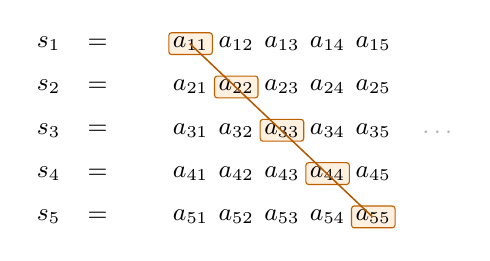
\begin{tikzpicture}[
  every node/.style={font=\small},
  digit/.style={font=\small},
  diagonal/.style={draw=orange!75!black, fill=orange!12, rounded corners=1pt, inner sep=1.5pt},
  guide/.style={orange!70!black, line width=0.55pt}
]
  \foreach \row/\name in {1/s_1,2/s_2,3/s_3,4/s_4,5/s_5} {
    \node[anchor=east] at (0,-0.55*\row) {$\name$};
    \node at (0.35,-0.55*\row) {$=$};
  }

  \foreach \row in {1,...,5} {
    \foreach \col in {1,...,5} {
      \node[digit] at (0.95+0.58*\col,-0.55*\row) {$a_{\row\col}$};
    }
  }

  \foreach \row in {1,...,5} {
    \node[diagonal] at (0.95+0.58*\row,-0.55*\row) {$a_{\row\row}$};
  }
  \draw[guide] (1.52,-0.55) -- (3.84,-2.75);

  \node[anchor=west, gray!60] at (4.35,-1.68) {$\cdots$};
\end{tikzpicture}

  \caption{Boxed entries $a_{nn}=s_n(n)$ whose bit flips define a sequence distinct from every listed row.}
  \label{fig:cantor-diagonal-binary-sequences}
\end{illustrationfigure}

Figure \ref{fig:cantor-diagonal-binary-sequences} marks the diagonal entries used in Theorem \ref{thm:binary-sequences-uncountable}.\\
Flipping the $n$th boxed bit forces $s(n)\neq s_n(n)$, so the constructed sequence cannot equal row $n$.


\subsection{Cardinal Comparison and the Continuum}

Throughout this subsection, assume Principle \ref{princ:axiom-of-choice-analysis} and use the initial-ordinal cardinality $\abs{X}$ from Definition \ref{def:cardinals-as-initial-ordinals}.

\begin{definition} \label{def:cardinal-comparison-and-arithmetic} \hlt{Cardinal Comparison and Arithmetic}\\
For sets $A,B$, define the \hlt{function set} by $A^B\defeq\{f\mid f:B\to A\}$. Let $\kappa,\lambda$ be cardinals.
\begin{enumerate}[label=(\roman*)]
\setlength{\itemsep}{0pt}
\item \hlt{Comparison}: the relations $\kappa\leq\lambda$ and $\kappa<\lambda$ are the corresponding ordinal comparisons.
\item The \hlt{cardinal sum} is $\kappa+\lambda\defeq\abs{(\{0\}\times\kappa)\cup(\{1\}\times\lambda)}$.
\item The \hlt{cardinal product} is $\kappa\lambda\defeq\abs{\kappa\times\lambda}$.
\item The \hlt{cardinal power} is $\kappa^\lambda\defeq\abs{\{f\mid f:\lambda\to\kappa\}}$.
\end{enumerate}
These are cardinal operations. Cardinal arguments distinguish them from the ordinal operations of Definition \ref{def:ordinal-arithmetic}.
\end{definition}

\begin{proposition} \label{prop:cardinal-operations-on-representatives} \hlt{Cardinal Comparison and Operations on Representatives}\\
Let $A,B$ be sets, and set $\kappa\defeq\abs{A}$ and $\lambda\defeq\abs{B}$.
\begin{enumerate}[label=(\roman*)]
\setlength{\itemsep}{0pt}
\item $\kappa\leq\lambda$ iff an injection $A\to B$ exists.
\item $\kappa<\lambda$ iff an injection $A\to B$ exists and $A\not\sim_{\#}B$.
\item $\kappa+\lambda=\abs{(\{0\}\times A)\cup(\{1\}\times B)}$. If $A\cap B=\emptyset$, then $\kappa+\lambda=\abs{A\cup B}$.
\item $\kappa\lambda=\abs{A\times B}$.
\item $\kappa^\lambda=\abs{A^B}$.
\end{enumerate}
\begin{proof}
Choose bijections $u:A\to\kappa$ and $v:B\to\lambda$ by Proposition \ref{prop:cardinality-canonical-and-bijection-invariant}(i).
\begin{enumerate}[label=(\roman*)]
\setlength{\itemsep}{0pt}
\item[$(i)$] ($\Rightarrow$) If $\kappa\leq\lambda$, then an injection $A\to B$ exists by Proposition \ref{prop:ordinal-cardinality-comparison}.
\item[$(i)$] ($\Leftarrow$) If an injection $A\to B$ exists, then $\kappa\leq\lambda$ by Proposition \ref{prop:ordinal-cardinality-comparison}.
\item[$(ii)$] ($\Rightarrow$) Suppose $\kappa<\lambda$. Then $\kappa\leq\lambda$ and $\kappa\neq\lambda$. An injection $A\to B$ exists by (i), and $A\not\sim_{\#}B$ by Proposition \ref{prop:cardinality-canonical-and-bijection-invariant}(ii).
\item[$(ii)$] ($\Leftarrow$) Suppose an injection $A\to B$ exists and $A\not\sim_{\#}B$. Then $\kappa\leq\lambda$ by (i) and $\kappa\neq\lambda$ by Proposition \ref{prop:cardinality-canonical-and-bijection-invariant}(ii), so $\kappa<\lambda$.
\item[$(iii)$] Set $U\defeq(\{0\}\times A)\cup(\{1\}\times B)$ and $V\defeq(\{0\}\times\kappa)\cup(\{1\}\times\lambda)$. Define $F:U\to V$ by $F(0,a)\defeq(0,u(a))$ and $F(1,b)\defeq(1,v(b))$.\\
The inverse sends $(0,\xi)$ to $(0,u^{-1}(\xi))$ and $(1,\eta)$ to $(1,v^{-1}(\eta))$, so $F$ is bijective by Theorem \ref{thm:bijective-iff-invertible-function}.\\
Hence $\abs{U}=\abs{V}$ by Proposition \ref{prop:cardinality-canonical-and-bijection-invariant}(ii), proving the first equality.\\
If $A\cap B=\emptyset$, define $G:U\to A\cup B$ by $G(0,a)\defeq a$ and $G(1,b)\defeq b$.\\
Its inverse sends $x\in A$ to $(0,x)$ and $x\in B$ to $(1,x)$, so $G$ is bijective. Thus $\kappa+\lambda=\abs{A\cup B}$ by Proposition \ref{prop:cardinality-canonical-and-bijection-invariant}(ii).
\item[$(iv)$] Define $P:A\times B\to\kappa\times\lambda$ by $P(a,b)\defeq(u(a),v(b))$. Its inverse is $(\xi,\eta)\mapsto(u^{-1}(\xi),v^{-1}(\eta))$, so $P$ is bijective by Theorem \ref{thm:bijective-iff-invertible-function}.\\
Therefore $\kappa\lambda=\abs{A\times B}$ by Proposition \ref{prop:cardinality-canonical-and-bijection-invariant}(ii).
\item[$(v)$] Define $T:A^B\to\{g\mid g:\lambda\to\kappa\}$ by $T(f)\defeq u\circ f\circ v^{-1}$. Its inverse sends $g:\lambda\to\kappa$ to $u^{-1}\circ g\circ v$, so $T$ is bijective by Theorem \ref{thm:bijective-iff-invertible-function}.\\
Hence $\kappa^\lambda=\abs{A^B}$ by Proposition \ref{prop:cardinality-canonical-and-bijection-invariant}(ii).
\end{enumerate}
\hlt{Structural Commentary}: Chosen bijections transport comparison and all three cardinal operations.\\
\hlt{Key Insight}: Bijections act coordinatewise on tags, pairs, and functions.
\end{proof}
\end{proposition}

\begin{definition} \label{def:continuum-cardinal} \hlt{Continuum Cardinal}\\
The \hlt{continuum cardinal} is $\mathfrak{c}\defeq2^{\aleph_0}$.
\end{definition}

\begin{proposition} \label{prop:continuum-cardinal-models} \hlt{Models of the Continuum Cardinal}\\
$\mathfrak{c}=\abs{\{0,1\}^{\N}}=\abs{\mathcal{P}(\N)}$.
\begin{proof}
The map $q:J_2\to\{0,1\}$ defined by $q(k)\defeq k-1$ is bijective. Thus $\abs{\{0,1\}}=2$ and $\abs{\N}=\aleph_0$ by Proposition \ref{prop:finite-cardinality-and-aleph-zero-agreement}(i),(iii).\\
Hence $\mathfrak{c}=\abs{\{0,1\}^{\N}}$ by Proposition \ref{prop:cardinal-operations-on-representatives}(v). The relation $\{0,1\}^{\N}\sim_{\#}\mathcal{P}(\N)$ holds by Proposition \ref{prop:binary-sequences-model-power-set}.\\
Hence $\abs{\{0,1\}^{\N}}=\abs{\mathcal{P}(\N)}$ by Proposition \ref{prop:cardinality-canonical-and-bijection-invariant}(ii).\\
\hlt{Structural Commentary}: Finite and countable representatives reduce cardinal exponentiation to binary functions and subsets.\\
\hlt{Key Insight}: A binary function is the characteristic function of one subset.
\end{proof}
\end{proposition}

\begin{corollary} \label{cor:continuum-strictly-exceeds-aleph-zero} \hlt{The Continuum Strictly Exceeds $\aleph_0$}\\
$\aleph_0<\mathfrak{c}$.
\begin{proof}
The map $j:\N\to\mathcal{P}(\N)$, $j(n)\defeq\{n\}$, is injective since $j(m)=j(n)\Rightarrow m=n$.\\
No bijection $\N\to\mathcal{P}(\N)$ exists by Theorem \ref{thm:cantor-power-set-theorem}. Therefore $\abs{\N}<\abs{\mathcal{P}(\N)}$ by Proposition \ref{prop:cardinal-operations-on-representatives}(ii).\\
The identities $\abs{\N}=\aleph_0$ and $\abs{\mathcal{P}(\N)}=\mathfrak{c}$ hold by Proposition \ref{prop:finite-cardinality-and-aleph-zero-agreement}(iii) and Proposition \ref{prop:continuum-cardinal-models}, respectively. Hence $\aleph_0<\mathfrak{c}$.\\
\hlt{Structural Commentary}: Singleton embedding gives weak comparison, while Cantor's theorem rules out equality.\\
\hlt{Key Insight}: The diagonal obstruction makes the continuum strictly larger.
\end{proof}
\end{corollary}


\subsection{Cardinal Arithmetic}

Throughout this subsection, assume Principle \ref{princ:axiom-of-choice-analysis} and use the cardinal operations from Definition \ref{def:cardinal-comparison-and-arithmetic}.

\begin{proposition} \label{prop:cardinal-arithmetic-reference-laws} \hlt{Cardinal Arithmetic Reference Laws}\\
Let $\kappa,\lambda,\mu$ be cardinals.
\begin{enumerate}[label=(\roman*)]
\setlength{\itemsep}{0pt}
\item $\kappa+\lambda=\lambda+\kappa$ and $\kappa\lambda=\lambda\kappa$.
\item $\kappa+(\lambda+\mu)=(\kappa+\lambda)+\mu$ and $\kappa(\lambda\mu)=(\kappa\lambda)\mu$.
\item $\kappa(\lambda+\mu)=\kappa\lambda+\kappa\mu$.
\item $\kappa^{\lambda+\mu}=\kappa^\lambda\kappa^\mu$, $(\kappa^\lambda)^\mu=\kappa^{\lambda\mu}$, and $(\kappa\lambda)^\mu=\kappa^\mu\lambda^\mu$.
\end{enumerate}
\begin{proof}
Set $A\defeq\{0\}\times\kappa$, $B\defeq\{1\}\times\lambda$, and $C\defeq\{2\}\times\mu$.\\
The sets are pairwise disjoint, and their coordinate projections are bijections onto $\kappa,\lambda,\mu$, respectively.\\
Thus $\abs{A}=\kappa$, $\abs{B}=\lambda$, and $\abs{C}=\mu$ by Proposition \ref{prop:cardinality-canonical-and-bijection-invariant}(ii) and Definition \ref{def:cardinals-as-initial-ordinals}.
\begin{enumerate}[label=(\roman*)]
\setlength{\itemsep}{0pt}
\item The identity is a bijection $A\cup B\to B\cup A$. The map $(a,b)\mapsto(b,a)$ is a bijection $A\times B\to B\times A$ with itself as inverse.
\item The equality $A\cup(B\cup C)=(A\cup B)\cup C$ holds.\\
The map $(a,(b,c))\mapsto((a,b),c)$ is a bijection $A\times(B\times C)\to(A\times B)\times C$ with inverse $((a,b),c)\mapsto(a,(b,c))$.
\item The equality $A\times(B\cup C)=(A\times B)\cup(A\times C)$ holds. The union on the right is disjoint because $B\cap C=\emptyset$.
\item Define $R:A^{B\cup C}\to A^B\times A^C$ by $R(f)\defeq(f|_B,f|_C)$. Its inverse is $R^{-1}(g,h)\defeq g\cup h$; disjointness makes this union a function.\\
Define $Q:(A^B)^C\to A^{B\times C}$ by $Q(F)(b,c)\defeq F(c)(b)$. Its inverse sends $h$ to $c\mapsto(b\mapsto h(b,c))$. Let $\pi_A(a,b)\defeq a$ and $\pi_B(a,b)\defeq b$.\\
The map $D:(A\times B)^C\to A^C\times B^C$ defined by $D(h)\defeq(\pi_A\circ h,\pi_B\circ h)$ has inverse $D^{-1}(f,g)(c)\defeq(f(c),g(c))$.
\end{enumerate}
Claims (i)--(iv) follow from these set equalities and bijections by Proposition \ref{prop:cardinal-operations-on-representatives}(iii)--(v).\\
\hlt{Structural Commentary}: Set identities and explicit bijections transport representative arithmetic to cardinal laws.\\
\hlt{Key Insight}: Restriction, currying, and projections control the exponent laws.
\end{proof}
\end{proposition}

\begin{theorem} \label{thm:infinite-cardinal-square-law} \hlt{Infinite Cardinal Square Law}\\
If $\kappa$ is an infinite cardinal, then $\abs{\kappa\times\kappa}=\kappa$.
\begin{proof}
\begin{enumerate}[label=(\roman*)]
\setlength{\itemsep}{0pt}
\item \hlt{Induction setup}: For an ordinal $\alpha$, let $P(\alpha)$ mean that, if $\alpha$ is an infinite cardinal, then $\abs{\alpha\times\alpha}=\alpha$.\\
Fix an ordinal $\kappa$ and assume $(\forall\beta<\kappa)\,P(\beta)$. It suffices by Principle \ref{princ:ordinal-foundations}(ii) to prove $P(\kappa)$.\\
The assertion $P(\kappa)$ is vacuous unless $\kappa$ is an infinite cardinal, so assume that it is.
\item \hlt{Well-order construction}: Define $r:\kappa\times\kappa\to\kappa$ by $r(\xi,\eta)\defeq\max\{\xi,\eta\}$.\\
For $p=(\beta,\beta')$ and $q=(\gamma,\gamma')$ in $\kappa\times\kappa$, declare $p\prec q$ when the first applicable condition holds:
\begin{enumerate}[label=(\alph*)]
\setlength{\itemsep}{0pt}
\item $r(p)<r(q)$;
\item $r(p)=r(q)$ and $\beta<\gamma$;
\item $r(p)=r(q)$, $\beta=\gamma$, and $\beta'<\gamma'$.
\end{enumerate}
Put $p\preceq q$ iff $p=q$ or $p\prec q$. Ordinal comparison makes these clauses exhaustive for distinct pairs.\\
Comparison by the first differing entry of $(r(p),\beta,\beta')$ is transitive and antisymmetric; hence $\preceq$ is a total order.\\
If $\emptyset\neq S\subseteq\kappa\times\kappa$, set $R_S\defeq\{r(p):p\in S\}$. The nonempty set $R_S$ has a least element $\rho$ by Principle \ref{princ:ordinal-foundations}(i).\\
Set $I_S\defeq\{\xi<\kappa:(\exists\eta<\kappa)\,[(\xi,\eta)\in S\land r(\xi,\eta)=\rho]\}$; it is nonempty by the definition of $\rho$.\\
The minimum $\xi_0\defeq\min I_S$ exists by Principle \ref{princ:ordinal-foundations}(i).\\
Set $J_S\defeq\{\eta<\kappa:(\xi_0,\eta)\in S\land r(\xi_0,\eta)=\rho\}$; it is nonempty by the definition of $I_S$.\\
The minimum $\eta_0\defeq\min J_S$ exists by Principle \ref{princ:ordinal-foundations}(i). Then $(\xi_0,\eta_0)$ is least in $S$, so $\preceq$ is a well-order.
\item \hlt{Ordinal comparison}: Choose an ordinal $\delta$ and an order isomorphism $f:(\delta,\leq)\to(\kappa\times\kappa,\preceq)$ by Principle \ref{princ:ordinal-foundations}(iii).\\
The map $\xi\mapsto(\xi,0)$ injects $\kappa$ into $\kappa\times\kappa$. Since $\abs{\kappa}=\kappa$ by Definition \ref{def:cardinals-as-initial-ordinals}, $\kappa\leq\abs{\kappa\times\kappa}$ by Proposition \ref{prop:ordinal-cardinality-comparison}.\\
The equality $\abs{\kappa\times\kappa}=\abs{\delta}$ holds by Proposition \ref{prop:cardinality-canonical-and-bijection-invariant}(ii), and $\abs{\delta}\leq\delta$ by Definition \ref{def:cardinals-as-initial-ordinals}. Thus $\kappa\leq\abs{\kappa\times\kappa}=\abs{\delta}\leq\delta$.
\item \hlt{Initial-segment contradiction}: Suppose $\kappa<\delta$. Write $f(\kappa)=(\beta,\beta')$ and set $X\defeq\{q\in\kappa\times\kappa:q\prec(\beta,\beta')\}$.\\
The restriction $f|_{\kappa}:\kappa\to X$ is bijective because $f$ preserves and reflects order.\\
Hence $\abs{X}=\kappa$ by Proposition \ref{prop:cardinality-canonical-and-bijection-invariant}(ii) and Definition \ref{def:cardinals-as-initial-ordinals}.\\
Set $\alpha\defeq\max\{\beta,\beta'\}+1$. Since $\beta,\beta'<\kappa$ and $\kappa$ is a limit ordinal by Lemma \ref{lem:infinite-cardinals-are-limit-ordinals}, $\alpha<\kappa$.\\
Set $\lambda\defeq\abs{\alpha}$. Then $\lambda$ is a cardinal, and a bijection $u:\alpha\to\lambda$ exists by Proposition \ref{prop:cardinality-canonical-and-bijection-invariant}(i).\\
Since $\lambda\leq\alpha$ by Definition \ref{def:cardinals-as-initial-ordinals}, $\lambda<\kappa$. If $q\in X$, then $r(q)\leq\max\{\beta,\beta'\}<\alpha$, so $q\in\alpha\times\alpha$.\\
The coordinate map $(\xi,\eta)\mapsto(u(\xi),u(\eta))$ is a bijection $\alpha\times\alpha\to\lambda\times\lambda$, whose restriction to $X$ is injective.\\
Thus $\kappa=\abs{X}\leq\abs{\lambda\times\lambda}$ by Proposition \ref{prop:ordinal-cardinality-comparison}. If $\lambda$ is finite, then $\abs{\lambda\times\lambda}<\aleph_0\leq\kappa$ by Theorem \ref{thm:multiplication-principle-finite-products} and Proposition \ref{prop:finite-cardinality-and-aleph-zero-agreement}.\\
If $\lambda$ is infinite, then $\abs{\lambda\times\lambda}=\lambda<\kappa$ by induction hypothesis. In either case, $\abs{\lambda\times\lambda}<\kappa$, contradicting $\kappa\leq\abs{\lambda\times\lambda}$; hence $\kappa\not<\delta$.
\item \hlt{Conclusion}: Since $\kappa\leq\delta$, $\delta=\kappa$ by Principle \ref{princ:ordinal-foundations}(i). Thus $f$ is a bijection $\kappa\to\kappa\times\kappa$, so $\abs{\kappa\times\kappa}=\kappa$ by Proposition \ref{prop:cardinality-canonical-and-bijection-invariant}(ii) and Definition \ref{def:cardinals-as-initial-ordinals}. Hence $P(\kappa)$ holds, completing the induction.
\end{enumerate}
\hlt{Structural Commentary}: Strong induction bounds max-ranked initial segments by smaller cardinal squares.\\
\hlt{Key Insight}: Every predecessor lies in a square of smaller cardinality.
\end{proof}
\end{theorem}

\begin{theorem} \label{thm:infinite-cardinal-absorption-reference} \hlt{Infinite Cardinal Absorption}\\
Let $\kappa,\lambda$ be cardinals, and let $\mu\defeq\max\{\kappa,\lambda\}$ be infinite.
\begin{enumerate}[label=(\roman*)]
\setlength{\itemsep}{0pt}
\item $\kappa+\lambda=\mu$.
\item If $\kappa,\lambda>0$, then $\kappa\lambda=\mu$.
\item $\aleph_0+\aleph_0=\aleph_0\aleph_0=\aleph_0$.
\end{enumerate}
\begin{proof}
The equality $\abs{\mu\times\mu}=\mu$ holds by Theorem \ref{thm:infinite-cardinal-square-law}. Set $U\defeq(\{0\}\times\mu)\cup(\{1\}\times\mu)$.\\
Since $0,1\in\mu$, the maps $\xi\mapsto(0,\xi)$ and $(i,\xi)\mapsto(\xi,i)$ inject $\mu$ into $U$ and $U$ into $\mu\times\mu$, respectively.\\
The identities $\abs{U}=\mu+\mu$ and $\abs{\mu}=\mu$ hold by Definition \ref{def:cardinal-comparison-and-arithmetic} and Definition \ref{def:cardinals-as-initial-ordinals}, respectively.\\
Thus $\mu\leq\mu+\mu\leq\abs{\mu\times\mu}=\mu$ by Proposition \ref{prop:ordinal-cardinality-comparison}, so $\mu+\mu=\mu$.
\begin{enumerate}[label=(\roman*)]
\setlength{\itemsep}{0pt}
\item Set $V\defeq(\{0\}\times\kappa)\cup(\{1\}\times\lambda)$. If $\mu=\kappa$, then $\xi\mapsto(0,\xi)$ injects $\mu$ into $V$; if $\mu=\lambda$, then $\xi\mapsto(1,\xi)$ does so.\\
The inclusions $\kappa\hookrightarrow\mu$ and $\lambda\hookrightarrow\mu$ induce an injection $V\to U$, and $\abs{V}=\kappa+\lambda$ by Definition \ref{def:cardinal-comparison-and-arithmetic}.\\
Thus $\mu\leq\kappa+\lambda\leq\mu+\mu=\mu$ by Proposition \ref{prop:ordinal-cardinality-comparison}, so $\kappa+\lambda=\mu$.
\item Assume $\kappa,\lambda>0$, so $0\in\kappa\cap\lambda$. If $\mu=\kappa$, then $\xi\mapsto(\xi,0)$ injects $\mu$ into $\kappa\times\lambda$; if $\mu=\lambda$, then $\xi\mapsto(0,\xi)$ does so.\\
The coordinate inclusions induce an injection $\kappa\times\lambda\to\mu\times\mu$, and $\kappa\lambda=\abs{\kappa\times\lambda}$ by Definition \ref{def:cardinal-comparison-and-arithmetic}.\\
Thus $\mu\leq\kappa\lambda\leq\abs{\mu\times\mu}=\mu$ by Proposition \ref{prop:ordinal-cardinality-comparison}, so $\kappa\lambda=\mu$.
\item The cardinal $\aleph_0$ is infinite by Proposition \ref{prop:finite-cardinality-and-aleph-zero-agreement}(iv). The asserted equalities follow by (i),(ii) with $\kappa=\lambda=\aleph_0$.
\end{enumerate}
\hlt{Structural Commentary}: The square law sandwiches each sum and nonzero product between $\mu$ and itself.\\
\hlt{Key Insight}: An infinite maximum absorbs every bounded factor.
\end{proof}
\end{theorem}


\section{Axiomatic and Advanced Set Theory}

This section reserves space for the deeper set-theoretic material suggested by the set-theory and metatheory contents: axioms, ordinals, models, forcing, large cardinals, and sets of reals.

\subsection{Ordinals, Transfinite Recursion, and Well-Foundedness}

\hlt{Placeholder}: Add well-founded relations, transitive sets, ordinal numbers, ordinal arithmetic, transfinite induction, and transfinite recursion.


\subsection{Models, Constructibility, and Independence}

\hlt{Placeholder}: Add models of set theory, the constructible universe, forcing previews, consistency strength, and independence statements.


\subsection{Filters, Ultrafilters, and Sets of Reals}

\hlt{Placeholder}: Add filters, ideals, ultrafilters, stationary/closed-unbounded sets, Borel and projective sets, descriptive set theory, and large-cardinal gateways.


\section{Mathematical Writing and Research Practice}

This section fixes the communication, evidence, integrity, and reading practices used to create and evaluate mathematical and machine-learning research.

\subsection{Theorem-Style Results and Formal Statements}

Formal environments advertise the role and authority of a block before the reader examines its details.

\begin{convention} \label{conv:theorem-style-result-hierarchy} \hlt{Theorem-Style Result Hierarchy}\\
The theorem-style category contains exactly the following proved results.
\begin{enumerate}[label=(\roman*)]
\setlength{\itemsep}{0pt}
\item \hlt{Theorem}: a major result that advances a principal objective of the surrounding work.
\item \hlt{Proposition}: an independently useful result of smaller local weight.
\item \hlt{Lemma}: a subsidiary result introduced primarily to support a later proof.
\item \hlt{Corollary}: a result requiring little additional argument after an earlier result.
\end{enumerate}
The classification communicates structural role rather than a universal rank of importance. Definitions introduce objects or terminology, while conjectures record unproved claims. This hierarchy follows standard mathematical-writing guidance \citep{mit1998mathematicalwriting}.
\end{convention}

\begin{process} \label{proc:theorem-statement-audit} \hlt{Theorem-Statement Construction and Audit}\\
Given a candidate result and its supporting argument, produce a statement that can be cited and proved without hidden context.
\begin{enumerate}[label=(\roman*)]
\setlength{\itemsep}{0pt}
\item \hlt{Purpose}: identify the reusable conclusion and its role in the dependency chain.
\item \hlt{Objects}: bind every ambient set, structure, parameter, map, and index before its first use.
\item \hlt{Hypotheses}: state the exact domain, regularity, finiteness, independence, or boundary conditions needed.
\item \hlt{Conclusion}: state existence, uniqueness, characterization, bound, convergence, or other claim explicitly.
\item \hlt{Claim census}: separate conclusions whose removal would erase a distinct proof obligation.
\item \hlt{Role}: choose theorem, proposition, lemma, or corollary by Convention \ref{conv:theorem-style-result-hierarchy}.
\item \hlt{Locality}: remove motivation, examples, proof machinery, and unused assumptions from the statement.
\item \hlt{Traceability}: attach a stable title and label, and cite external ownership of a nonoriginal result.
\end{enumerate}
The final statement should remain intelligible when read apart from the preceding paragraph. Self-contained statements and first-use symbol definitions are central expository checks \citep{knuth1988mathematicalwriting}.
\end{process}

\begin{principle} \label{princ:claim-authority-separation} \hlt{Claim--Authority Separation}\\
A formal block should display its actual epistemic status. A definition stipulates meaning; an assumption declares a condition; a conjecture remains unproved; a theorem-style result requires a proof; and an empirical statement requires data and a protocol. A citation identifies prior ownership but does not replace a proof when the present work claims to establish the result.
\end{principle}

\begin{warning} \label{warn:statement-proof-contamination} \hlt{Statement--Proof Contamination}\\
Do not place a proof plan, auxiliary construction, example, or claim of obviousness inside a theorem-style statement. Such material obscures the logical contract, creates unused hypotheses, and makes later citation unreliable. Move proof-specific objects into the proof and explanatory material after the formal owner.
\end{warning}


\subsection{Proof Construction and Revision}

A proof is a checkable argument from declared hypotheses, definitions, and earlier proved results to the exact stated conclusion.

\begin{proofmethod} \label{meth:proof-construction-audit} \hlt{Proof Construction and Audit}\\
Given a theorem-style statement, construct and review its proof as follows.
\begin{enumerate}[label=(\roman*)]
\setlength{\itemsep}{0pt}
\item \hlt{Parse}: expose the objects, hypotheses, quantifier dependencies, and conclusion by Proof Method \ref{meth:proof-grammar}.
\item \hlt{Plan}: select a direct argument, cases, two inclusions, induction, contradiction, construction, or another fitting architecture.
\item \hlt{Dependencies}: list only earlier results whose hypotheses can be verified at the point of citation.
\item \hlt{Obligations}: map each numbered claim, implication direction, existence witness, and uniqueness assertion to a proof unit.
\item \hlt{Execution}: introduce variables before use and justify each inference by a definition, calculation, hypothesis, or earlier result.
\item \hlt{Boundaries}: handle empty, zero, singular, endpoint, and other degenerate cases that affect an argument.
\item \hlt{Closure}: verify that the final sentence discharges the original conclusion rather than a nearby surrogate.
\item \hlt{Cold read}: reread without relying on memory; test notation, citations, and transitions as a skeptical reader would.
\end{enumerate}
The proof should expose its plan when the route is not apparent, yet retain every step needed for verification. Mathematical-writing guidance likewise emphasizes status, motivation, and conceptual structure \citep{mit1998mathematicalwriting,knuth1988mathematicalwriting}.
\end{proofmethod}

\begin{process} \label{proc:proof-revision-passes} \hlt{Proof Revision Passes}\\
Revise a completed proof in three passes.
\begin{enumerate}[label=(\roman*)]
\setlength{\itemsep}{0pt}
\item \hlt{Validity}: check every dependency, implication, case split, witness, index, limit, and exceptional case.
\item \hlt{Architecture}: align proof units with statement claims and make long operative stages visible.
\item \hlt{Exposition}: remove repetition, bind notation earlier, compress routine algebra, and expand decisive unfamiliar steps.
\end{enumerate}
Typography is reviewed only after the mathematical and logical structure is stable.
\end{process}

\begin{warning} \label{warn:evidence-is-not-proof} \hlt{Evidence Is Not Proof}\\
Finite testing, a diagram, numerical agreement, or a successful program run supports only the cases and conditions examined. None closes an unrestricted quantified claim without an exhaustive argument and a proof that the enumeration is complete. Computation may discover a conjecture, locate a counterexample, or verify a formally specified finite case.
\end{warning}

\begin{principle} \label{princ:proof-detail-proportionality} \hlt{Proof Detail Proportionality}\\
Detail belongs where correctness or understanding depends on it. Expand novel constructions, fragile estimates, changes of quantifier, and boundary arguments; compress familiar algebra only while the remaining chain is checkable. The goal is neither maximal formality nor persuasive rhetoric, but a reproducible mathematical argument.
\end{principle}


\subsection{Methods, Algorithms, and Computational Artifacts}

Procedural blocks must distinguish conceptual guidance, executable steps, and claims about correctness or performance.

\begin{convention} \label{conv:procedural-environment-roles} \hlt{Procedural Environment Roles}\\
Use the following roles throughout these notes.
\begin{enumerate}[label=(\roman*)]
\setlength{\itemsep}{0pt}
\item \hlt{Proof method}: a reusable proof route, reduction, recognition criterion, or obligation checklist.
\item \hlt{Computation method}: a reusable construction, calculation, approximation, diagnostic, or test.
\item \hlt{Method}: a short convention, classification workflow, or inseparable hybrid with no clearer subtype.
\item \hlt{Process}: an organizational workflow for research, writing, review, or documentation.
\item \hlt{Algorithm}: executable pseudocode with declared inputs, outputs, control flow, and termination conditions.
\end{enumerate}
A worked instance belongs in an example, an actual proof in a proof, and implementation-specific behavior in code or an artifact record.
\end{convention}

\begin{process} \label{proc:algorithm-specification-audit} \hlt{Algorithm Specification and Audit}\\
Before publishing pseudocode, record its contract and verification obligations.
\begin{enumerate}[label=(\roman*)]
\setlength{\itemsep}{0pt}
\item \hlt{Problem}: state the task and the abstraction level at which the algorithm operates.
\item \hlt{Input}: specify types, dimensions, admissibility, representation, and malformed-input behavior.
\item \hlt{Output}: specify the returned object and a postcondition that characterizes success.
\item \hlt{State}: define initialization, mutable state, randomness, and any invariant needed for correctness.
\item \hlt{Steps}: write one unambiguous action per step with readable branches and loops.
\item \hlt{Termination}: state the stopping rule and justify termination when it is claimed.
\item \hlt{Correctness}: separate the proof of the postcondition from the pseudocode itself.
\item \hlt{Resources}: state complexity only with an input-size parameter, cost model, resource, and case type.
\item \hlt{Limits}: record numerical, memory, precision, platform, approximation, and applicability boundaries.
\end{enumerate}
Labeled steps and explanatory invariants clarify the distinction between an algorithm and program text \citep{knuth1988mathematicalwriting}.
\end{process}

\begin{principle} \label{princ:formal-informal-procedural-pair} \hlt{Formal and Informal Procedural Views}\\
Complex procedures often need complementary views. The formal view fixes inputs, outputs, updates, and stopping conditions; the informal view explains the invariant, decomposition, or design choice. Neither should duplicate the other, and only a separate proof can establish mathematical correctness.
\end{principle}

\begin{process} \label{proc:computational-artifact-record} \hlt{Computational Artifact Record}\\
For code supporting a reported result, archive the source revision, dependencies, runtime, platform, configuration, random seeds, data identifiers, licenses, commands, and expected outputs. Map each reported figure, table, or metric to the command that creates it. State unavailable components and access restrictions explicitly. Current ML reporting guidance requests exact execution instructions and enough experimental detail to interpret the main results \citep{neurips2026checklist}.
\end{process}

\begin{warning} \label{warn:algorithm-evidence-boundaries} \hlt{Algorithm Evidence Boundaries}\\
Passing tests does not establish correctness outside the tested cases, and an asymptotic bound does not predict wall-clock performance without a cost model and operating conditions. Keep specification, proof, implementation, benchmark, and interpretation as distinct evidence types.
\end{warning}


\subsection{Mathematical Research and Integrity}

Mathematical research alternates discovery, attempted refutation, proof, verification, and communication rather than proceeding linearly from question to theorem.

\begin{process} \label{proc:mathematical-research-cycle} \hlt{Mathematical Research Cycle}\\
For a proposed research problem, maintain a revisable cycle with the following stages.
\begin{enumerate}[label=(\roman*)]
\setlength{\itemsep}{0pt}
\item \hlt{Question}: state the object, scope, known assumptions, and a falsifiable or provable target.
\item \hlt{Literature}: identify definitions, known results, counterexamples, adjacent formulations, and open status.
\item \hlt{Exploration}: compute examples, boundary cases, and nonexamples while recording the tested domain.
\item \hlt{Conjecture}: state the strongest precise claim supported by exploration, with all suspected hypotheses.
\item \hlt{Attack}: search independently for a proof and a counterexample; record failed routes and new obstructions.
\item \hlt{Revision}: weaken, strengthen, split, or reframe the conjecture when an example or proof obligation demands it.
\item \hlt{Verification}: check every proof dependency, compare with prior results, and seek independent criticism.
\item \hlt{Communication}: state novelty accurately, write a complete proof, cite provenance, and record limitations.
\end{enumerate}
MIT's project laboratory similarly presents mathematical discovery as data generation, conjecture, experiment, proof or counterexample, and writing \citep{mit2013projectlaboratory}.
\end{process}

\begin{process} \label{proc:research-claim-ledger} \hlt{Research Claim Ledger}\\
Maintain one row per substantive claim with its exact wording, status, evidence, dependencies, source locator, and unresolved checks. Distinguish proved, conjectured, computed, observed, reproduced, replicated, and interpreted claims. Update the row when a hypothesis, dataset, code revision, or conclusion changes. This record prevents an exploratory observation from silently becoming a theorem or empirical conclusion.
\end{process}

\begin{convention} \label{conv:reproducibility-replicability-generalizability} \hlt{Reproducibility, Replicability, and Generalizability}\\
Use the National Academies terminology \citep{nasem2019reproducibility}.
\begin{enumerate}[label=(\roman*)]
\setlength{\itemsep}{0pt}
\item \hlt{Reproducibility}: consistent computational results from the same data, code, methods, and analysis conditions.
\item \hlt{Replicability}: consistent results from a new study addressing the same question with newly obtained data.
\item \hlt{Generalizability}: applicability of a result to contexts or populations beyond those directly studied.
\end{enumerate}
These are separate targets. A reproducible computation need not replicate on new data or generalize to a new setting.
\end{convention}

\begin{principle} \label{princ:research-integrity-record} \hlt{Research Integrity and Stewardship}\\
Research records should permit scrutiny, correction, and appropriate reuse. Report methods and findings honestly; preserve accurate records; credit contributions and prior work; disclose conflicts; respect confidentiality, consent, licenses, and governing rules; and correct the record when an error is found. These duties reflect the honesty, accountability, fairness, and stewardship principles of the Singapore Statement \citep{singapore2010integrity}.
\end{principle}

\begin{warning} \label{warn:novelty-and-negative-results} \hlt{Novelty and Negative Results}\\
Do not equate novelty with truth or publication with correctness. Search for prior and concurrent work before claiming priority, and report a failed proof, null result, or nonreplication with its actual protocol and uncertainty. A negative outcome may diagnose a false conjecture, an inadequate method, or a boundary of generality; the evidence must distinguish these possibilities.
\end{warning}


\subsection{Machine Learning and AI Research}

Machine-learning and AI claims combine statistical, computational, system, and social evidence, so the study design must identify which authority supports each conclusion.

\begin{process} \label{proc:ml-ai-study-protocol} \hlt{Machine-Learning and AI Study Protocol}\\
Design an empirical study before interpreting its scores.
\begin{enumerate}[label=(\roman*)]
\setlength{\itemsep}{0pt}
\item \hlt{Question}: state the population, task, context of use, intervention or comparison, and claimed outcome.
\item \hlt{Claim type}: classify each target as theoretical, empirical, causal, computational, system, or normative.
\item \hlt{Data}: record provenance, version, license, collection, consent or access status, labels, exclusions, and preprocessing.
\item \hlt{Evaluation boundary}: protect test data from training, model selection, prompt design, preprocessing, and human iteration.
\item \hlt{Comparators}: choose relevant baselines, ablations, and resource-matched alternatives before inspecting final results.
\item \hlt{Protocol}: fix splits, metrics, hyperparameter selection, seeds, stopping rules, hardware, software, and compute budget.
\item \hlt{Uncertainty}: repeat stochastic runs and report the source and calculation of intervals, variation, or significance measures.
\item \hlt{Stress tests}: examine subgroups, shift, robustness, failure modes, sensitivity, and plausible misuse within scope.
\item \hlt{Artifacts}: preserve code, data handles, checkpoints, configurations, logs, and command-to-result mappings.
\item \hlt{Report}: separate observed results from interpretation and state limitations, costs, risks, and unsupported generalizations.
\end{enumerate}
The NeurIPS checklist and its reproducibility program emphasize assumptions, complete proofs, experimental details, uncertainty, artifacts, ethics, and limitations \citep{neurips2026checklist,pineau2021reproducibility}.
\end{process}

\begin{process} \label{proc:ml-artifact-documentation} \hlt{Dataset and Model Documentation}\\
Release documentation with each durable ML artifact.
\begin{enumerate}[label=(\roman*)]
\setlength{\itemsep}{0pt}
\item \hlt{Dataset}: record motivation, composition, collection, preprocessing, labeling, intended uses, restrictions, and maintenance.
\item \hlt{Model}: record identity, version, intended and excluded uses, training data, evaluation protocol, subgroup results, and limitations.
\item \hlt{System}: record interfaces, human roles, deployment assumptions, monitoring, update policy, safeguards, and rollback conditions.
\end{enumerate}
Dataset datasheets and model cards establish complementary documentation patterns for provenance, intended use, evaluation, and limitations \citep{gebru2021datasheets,mitchell2019modelcards}.
\end{process}

\begin{principle} \label{princ:contextual-ai-risk} \hlt{Contextual AI Risk Assessment}\\
Accuracy alone is not a complete system claim. For the intended context, select and justify tests for validity and reliability, safety, security and resilience, accountability and transparency, explainability and interpretability, privacy, and harmful-bias management. These characteristics can conflict and require documented tradeoffs. This versioned vocabulary follows the voluntary NIST AI RMF 1.0 \citep{tabassi2023airmf}.
\end{principle}

\begin{warning} \label{warn:ml-evaluation-leakage} \hlt{Adaptive Evaluation and Leakage}\\
Any choice influenced by protected evaluation data makes the final score adaptive. Repeated leaderboard queries, test-set debugging, manual example selection, and unreported prompt tuning can all leak evaluation information. Reserve a final assessment boundary or disclose the adaptation and narrow the claim.
\end{warning}

\begin{warning} \label{warn:ml-benchmark-overclaiming} \hlt{Benchmark Overclaiming}\\
A higher score supports a claim only under the reported dataset, metric, resources, selection procedure, and uncertainty. It does not by itself establish practical usefulness, causal benefit, robustness, fairness, safety, or superiority in another operating environment.
\end{warning}


\subsection{Reading and Synthesizing Research Papers}

Reading depth should match the decision at hand: triage, comprehension, verification, reproduction, or synthesis.

\begin{process} \label{proc:three-pass-paper-reading} \hlt{Three-Pass Paper Reading}\\
Adapt the three-pass method of \citet{keshav2007readpaper} to the paper's evidence type.
\begin{enumerate}[label=(\roman*)]
\setlength{\itemsep}{0pt}
\item \hlt{Triage}: inspect title, abstract, introduction, headings, conclusion, figures, and references. Record category, context, claimed contribution, apparent assumptions, and relevance.
\item \hlt{Comprehension}: read the body carefully, map each main claim to its stated evidence, inspect figures and tables, and mark unfamiliar prerequisites or missing details.
\item \hlt{Reconstruction}: independently rebuild the proof, derivation, algorithm, or experiment closely enough to expose hidden assumptions, fragile steps, and reproducibility barriers.
\end{enumerate}
Stop after the earliest pass sufficient for the decision, and resume only after acquiring a missing prerequisite when further reading would otherwise be guesswork.
\end{process}

\begin{process} \label{proc:paper-claim-evidence-ledger} \hlt{Paper Claim--Evidence Ledger}\\
Create one entry per central claim and record its locator, exact scope, assumptions, evidence type, dependency, result, uncertainty, and limitation. For a mathematical paper, reconstruct definitions and proof obligations. For an empirical paper, reconstruct the sample, protocol, comparator, metric, variability, and analysis. For a systems paper, reconstruct the boundary, workload, implementation, platform, and failure model. Mark each claim as supported, partially supported, unsupported, or not assessed; reputation and venue are metadata rather than evidence.
\end{process}

\begin{process} \label{proc:literature-synthesis} \hlt{Literature Search and Synthesis}\\
Build a literature map rather than a pile of summaries.
\begin{enumerate}[label=(\roman*)]
\setlength{\itemsep}{0pt}
\item \hlt{Seed}: start from precise keywords, a recent survey, and several directly relevant papers.
\item \hlt{Backward search}: follow repeated foundational citations to original results, data, or methods.
\item \hlt{Forward search}: locate corrections, replications, extensions, and critiques that cite each key work.
\item \hlt{Cluster}: group papers by question, assumptions, method, evidence, and operating context rather than by author.
\item \hlt{Compare}: normalize terminology and record agreements, contradictions, gaps, and incomparable protocols.
\item \hlt{Saturate}: stop when new searches cease changing the conceptual map, while retaining the search date and boundary.
\end{enumerate}
Keshav's survey procedure likewise expands seed papers through repeated authors, shared references, and recent proceedings \citep{keshav2007readpaper}.
\end{process}

\begin{warning} \label{warn:paper-version-and-source-status} \hlt{Version and Source Status}\\
Before relying on a paper, check its version, venue, peer-review status, corrections, retractions, supplements, artifact links, and conflicts of interest. Cite the original source for a result or dataset when available. A preprint may be valuable, and peer review may improve reliability, but neither status settles the truth of a claim.
\end{warning}

\begin{principle} \label{princ:read-against-the-claim} \hlt{Read Against the Claim}\\
Evaluate the strongest wording in the title, abstract, or conclusion against the narrowest evidence in the body. The decisive questions are what was established, under which assumptions, by which evidence, with what uncertainty, and within which boundary.
\end{principle}


